%*************************************************************************
% Dokument Einstellungen
%*************************************************************************
\documentclass[fontsize=12pt,paper=a4,open=any,parskip=half,
  twoside=false,toc=listof,toc=bibliography,fleqn,leqno,
  captions=nooneline,captions=tableabove,british]{scrbook}
%*************************************************************************
% Importieren von Paketen die benutzt werden
%*************************************************************************
\usepackage[utf8]{inputenc} % load early
\usepackage[T1]{fontenc}    % load early
\usepackage[ngerman]{babel}
\usepackage[autostyle=true]{csquotes}
\usepackage{graphicx, booktabs, float, scrhack}
\usepackage{wrapfig}
\usepackage{caption}
\usepackage{listings, lstautogobble}
%\usepackage{fancyref}
%\usepackage{showkeys}
\usepackage[svgnames]{xcolor}
\usepackage{amsmath,amssymb}
\usepackage[automark]{scrlayer-scrpage}
\usepackage[backend=biber,style=numeric]{biblatex} %,sortcase=false,
\usepackage{url}
\usepackage[nohyperlinks]{acronym}
\usepackage{etoolbox}
\usepackage{hyphenat}

%*************************************************************************
% Bibliographies - Zitatquellen
%*************************************************************************
\addbibresource{Projekt.bib}

%*************************************************************************
% Weitere Dokument Einstellungen
%*************************************************************************
\PassOptionsToPackage{hyphens}{url} 
\usepackage[hidelinks]{hyperref}  % load late
\setkomafont{disposition}{\sffamily}
\setcounter{secnumdepth}{3}
\addtocontents{toc}{\setcounter{tocdepth}{1}}
\hyphenation{every-where}

\setcounter{biburllcpenalty}{7000}
\setcounter{biburlucpenalty}{8000}

%*************************************************************************
% Dokumentanfang
%*************************************************************************
\begin{document}
%Aktivierung römische Seitenzahlen
\frontmatter

%Titelblatt Einstellungen
\titlehead{% siehe KOMA-Script-Anleitung
  \begin{minipage}[t]{0.65\textwidth}
    \raggedright
    			Frankfurt University of Applied Sciences\\
				Fachbereich 2: Informatik und Ingenieurwissenschaften\\
				Studiengang: Informatik (B.Sc.)\\
  \end{minipage}
  \hfill
  \raisebox{-\dimexpr\totalheight-\ht\strutbox\relax}{
    
\includegraphics[width=5cm]{Bilder/fra-uas}
  }
}

\subject{Projektarbeit}
\title{Software-defined Networking mit Openflow}
\subtitle{}
\author{Mücahit Sagiroglu\\
Matrikelnummer: 1228852\\
James Belmonte\\
Matrikelnummer: 1340604\\
Naghmeh Ghavidel Rostami\\
Matrikelnummer: 1249307\\
Tung Trinh\\
Matrikelnummer: 1320718\\
}
\date{Vorgelegt am: 10. Februar 2022}
\publishers{Dozent: Maurizio Petrozziello\\
Modul 25: Informatik Projekt\\
Software-defined Networking mit Openflow\\
Wintersemester 2021/2022\\
}

\maketitle
%Eigenständigkeitserklärung
\chapter*{Eigenständigkeitserklärung}
Hiermit erklären wir, dass wir die vorliegende Arbeit eigenständig verfasst, keine anderen als die
angegebenen Quellen und Hilfsmittel verwendet sowie die aus fremden Quellen direkt oder indirekt
übernommenen Stellen/Gedanken als solche kenntlich gemacht haben. Diese Arbeit wurde noch keiner
anderen Prüfungskommission in dieser oder einer ähnlichen Form vorgelegt. Sie wurde bisher auch nicht
veröffentlicht.

Hiermit stimmen wir zu, dass die vorliegende Arbeit von der Prüferin/ dem Prüfer in elektronischer Form
mit entsprechender Software auf Plagiate überprüft wird.

\begin{figure}[H]
	\centering
	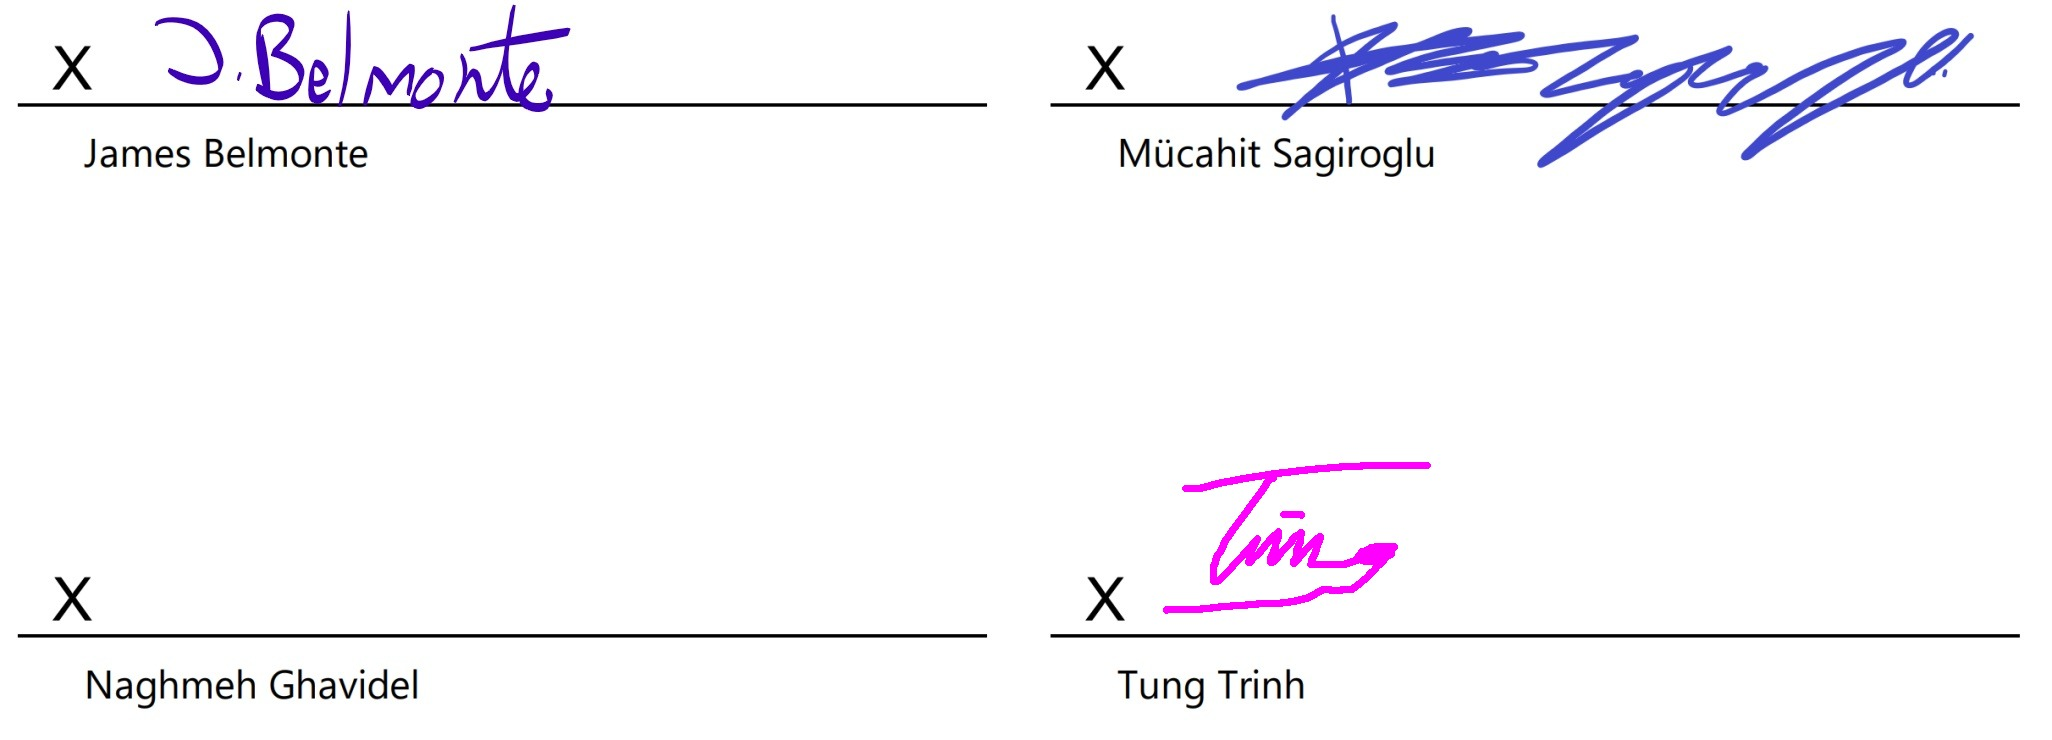
\includegraphics[width=1\linewidth]{Bilder/unterschrift}
\end{figure}

%Inhaltsverzeichnes & Abbildungsverzeichnis & Tabellenverzeichnis
\tableofcontents
\listoffigures
\listoftables
\lstlistoflistings
%ABKÜRZUNGSVERZECIHNIS
\chapter{Abkürzungsverzeichnis}
\begin{acronym}
	\acro{k}[ADSL]{Asymmetric Digital Subscriber Line}
	\acro{k}[API]{application programming interface}
	\acro{k}[bzw.]{beziehungsweise}
	\acro{k}[CLI]{Command Line Interface}
	\acro{k}[DHCP]{Dynamic Host Configuration Protocol}
	\acro{k}[DNS]{Domain Name System}
	\acro{k}[ESP]{Encapsulating Security Payload}
	\acro{k}[HTTP]{Hypertext Transfer Protocol }
	\acro{k}[HTTPS]{Hypertext Transfer Protocol Secure}
	\acro{k}[ISP]{Internet Service Provider}
	\acro{k}[LAN]{Local Area Network}
	\acro{k}[MTU]{Maximum Transmission Unit}
	\acro{k}[NAT]{Network Address Translation}
	\acro{k}[OF]{OpenFlow}
	\acro{k}[OSI-Modell]{Open Systems Interconnection model}
	\acro{k}[SDN]{Software Defined Network}
	\acro{k}[SDSL]{Symmetric Digital Subscriber Line}
	\acro{k}[usw.]{und so weiter}
	\acro{k}[VPN]{Virtual Private Network}
	\acro{k}[WAN]{Wide Area Network}
\end{acronym}


%Kapitel: Einleitung
\chapter{Abstract}
{\tiny Verfasst von: Tung\par}
Der vorliegende Projektbericht dient als Dokumentation des Informatikprojekts „Software-Defined Network mit OpenFlow“ an der Frankfurt University of Applied Sciences im Bachelorstudiengang Informatik im Wintersemester 2021/2022.\par
Das Aufkommen des Internets hat eine Revolution in der Informationstechnologie geschaffen. Durch eine neue Art der Kommunikation kann der Mensch auf nationaler wie auch auf internationaler Ebene effizienter und effektiver Informationen weitervermitteln. Dies bildet die Grundlage für die heutige Wissensökonomie.\par
Die traditionelle Netzwerkarchitektur ist jedoch seit einem halben Jahrhundert unverändert geblieben und wird für die Geschäftsanforderungen von Unternehmen, Netzwerkbetreibern und Endbenutzern zunehmend ungeeignet. Gegenwärtig werden die Geschäftsanforderungen von Unternehmen immer komplexer und die Anwendungsvielfalt der Endbenutzer nimmt zu, was zu unterschiedlichen Anforderungen der Benutzer an Verbindungsnetzwerke führt. Das Netzwerk muss auf sich schnell ändernde Parameter von Latenz, Bandbreite, Routing, Sicherheit und so weiter (usw.) entsprechend den Anforderungen der Anwendungen reagieren \cite{case}.\par
In den letzten Jahren hat die dramatische Zunahme der Netzwerkkomplexität Schwierigkeiten bei der traditionellen Netzwerkadministration mit sich gebracht. Das Konfigurieren von Computernetzwerksystemen unter Verwendung vordefinierter Richtlinien, das Rekonfigurieren von Netzwerken, um auf Änderungen zu reagieren, die Fehlerkorrektur und der Lastausgleich sind zu gewaltigen Aufgaben geworden. Wenn die Parameter des Netzwerks neu konfiguriert wurden, musste jedes Gerät manuell vollständig neu konfiguriert werden, anstatt einfach nur den Teil der Steuerungsebene zu ändern (vgl. Kim/Feamster 2013: 114f). Dies führte zu einem revolutionären Wandel in der Netzwerktechnologie durch die Zentralisierung der Netzwerkadministration. Seitdem wurde das Konzept des Software-Defined Network (SDN) geboren \cite[114-115]{improve}. 

%Aktivierung arabische Seitenzahlen
\mainmatter % Seite fängt mit 1 an
\chapter{Software-defined Networking}\label{sdn}
Im folgenden Abschnitt werden die jeweiligen Einleitungen jedes Mitgliedes vorgestellt. Sie dienen als separate Einleitungen zum Projektbericht.

\section*{Einleitung von James}\label{einl-james}
\begin{wrapfigure}{r}{0.4\textwidth}
	\vspace{-\baselineskip}
	\centering
	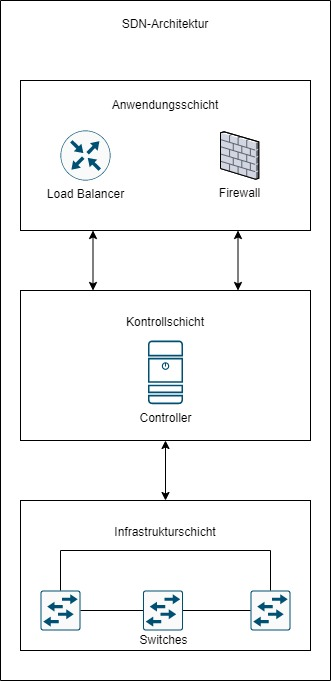
\includegraphics[width=0.23\textwidth]{Bilder/layer1}
	\caption{SDN Architektur}
	\label{layer1}
\end{wrapfigure}
Gegenwärtig gibt es im Bereich der Verwaltung von Computernetzwerken viele neue komplexe Anforderungen und notwendige Konfigurationen, die berücksichtigt werden müssen.  Der Datenaustausch innerhalb eines Netzwerkes ist um ein Vielfaches gestiegen, somit steigt die Auslastung das ein Netzwerksystem aushalten muss. Bei einem traditionellen Netzwerk würde das heißen, dass ein Netzwerkadministrator alle Netzwerkkomponenten wie Router, Switches und Firewalls etc. manuell konfigurieren müsste, um allen entsprechenden Anforderungen zu verwirklichen. Ferner müssen Netzwerkadministratoren viel Zeit in die Konfiguration legen, um alles korrekt zu implementieren.\par
Software Defined Networking bietet hierzu eine Alternativmöglichkeit zur Verwaltung einer Netzwerkumgebung. Im Gegensatz zu traditionellen Netzwerken trennt SDN die Kontrollschicht und die Datenschicht, und ermöglicht dadurch die Kontrolle des Netwerkes über das Netz. Im Mittelpunkt des Netzwerkes befindet sich ein SDN-Controller, der zur Konfiguration von allen Netzwerkkomponenten genutzt wird \cite{sdn1}. Die SDN-Architektur ist auf drei Ebenen aufgeteilt und wird anhand von Abbildung \ref{layer1} nochmals visuell dargestellt. Die Anwendungsschicht enthält Applikationen für SDN wie Firewall und Loadbalancer und wird mithilfe der REST API bereitgestellt \cite{james1}. Die Kontrollschicht enthält den SND-Controller, worüber das gesamte Netzwerk gesteuert wird. Die Infrastrukturschicht enthält die Netzwerkkomponenten wie Switches und Router und sind mit dem SDN-Controller verbunden, um die eingestellten Anforderungen vom Controller durchzusetzen. Die Architektur enthält mehrere Schnittstellen, sowohl eine Northbound API zwischen Anwendungsschicht und Kontrollschicht als auch eine Soutbound API zwischen Kontrollschicht und Infrastrukturschicht. Die Datenübertragung beim Southbound API erfolgt mit OpenFlow Protokolle. Bei der Weiterleitung eines Datenpakets wird die Weiterleitung auf der Datenschicht von einem Switch oder einem Router aufgenommen. Der SDN-Controller, der sich auf der Kontrollschicht befindet, entscheidet, wie das Datenpaket weitergeleitet wird \cite{james1}. Dadurch können verschiedene Netzwerkfunktionen implementiert werden, die von den Switches und Routern umgesetzt werden müssen. Die Kommunikation zwischen dem SDN-Controller und den Switches in der Infrastrukturschicht wird durch Openflow realisiert. Durch die Änderung des flow tables im Switch, kann der Controller das Verhalten des Switches beeinflussen und so einstellen, dass die Instruktionen des Controllers umgesetzt werden \cite{james1}. Im Gegensatz zu der traditionellen Weise die Netzwerkkomponenten manuell zu konfigurieren, kann durch die Trennung von Kontrollschicht und Datenschicht der Controller genutzt werden, um alle Konfigurationen von Komponenten im Netzwerk umzusetzen \cite{james3}. Zudem kann durch das zentrale Management des Netzwerkes und das der SDN-Controller programmierbar ist, ein Administrator effizienter, flexibler und agiler Handeln \cite{james1}. Besonders im Bereich Quality of Service muss ein Netzwerk agiler und flexibler als in der Vergangenheit sein. Somit kann Quality of Service mit SDN gewährleistet und einfacher umgesetzt werden \cite{james5}.Logischerweise kann auch argumentiert werden, dass durch das zentrale Management über das Netz geringere Betriebskosten aufkommen, da die Konfigurationsänderungen effizienter umgesetzt werden können.  Jedoch ist ein erwähnenswerter Nachteil, dass beim Ausfall eines SDN-Controllers in einem Netzwerk das gesamte Netzwerk ausfällt. Dies könnte durch eine Denial of Service attack ausgelöst werden. Somit könnte die Möglichkeit bestehen, mehrere Ausweichcontroller für solche Ereignisse vorzubereiten.
\newpage
\section*{Einleitung von Mücahit}\label{einl-müco}
\begin{wrapfigure}{r}{0.4\textwidth}
	\vspace{-\baselineskip}
	\centering
	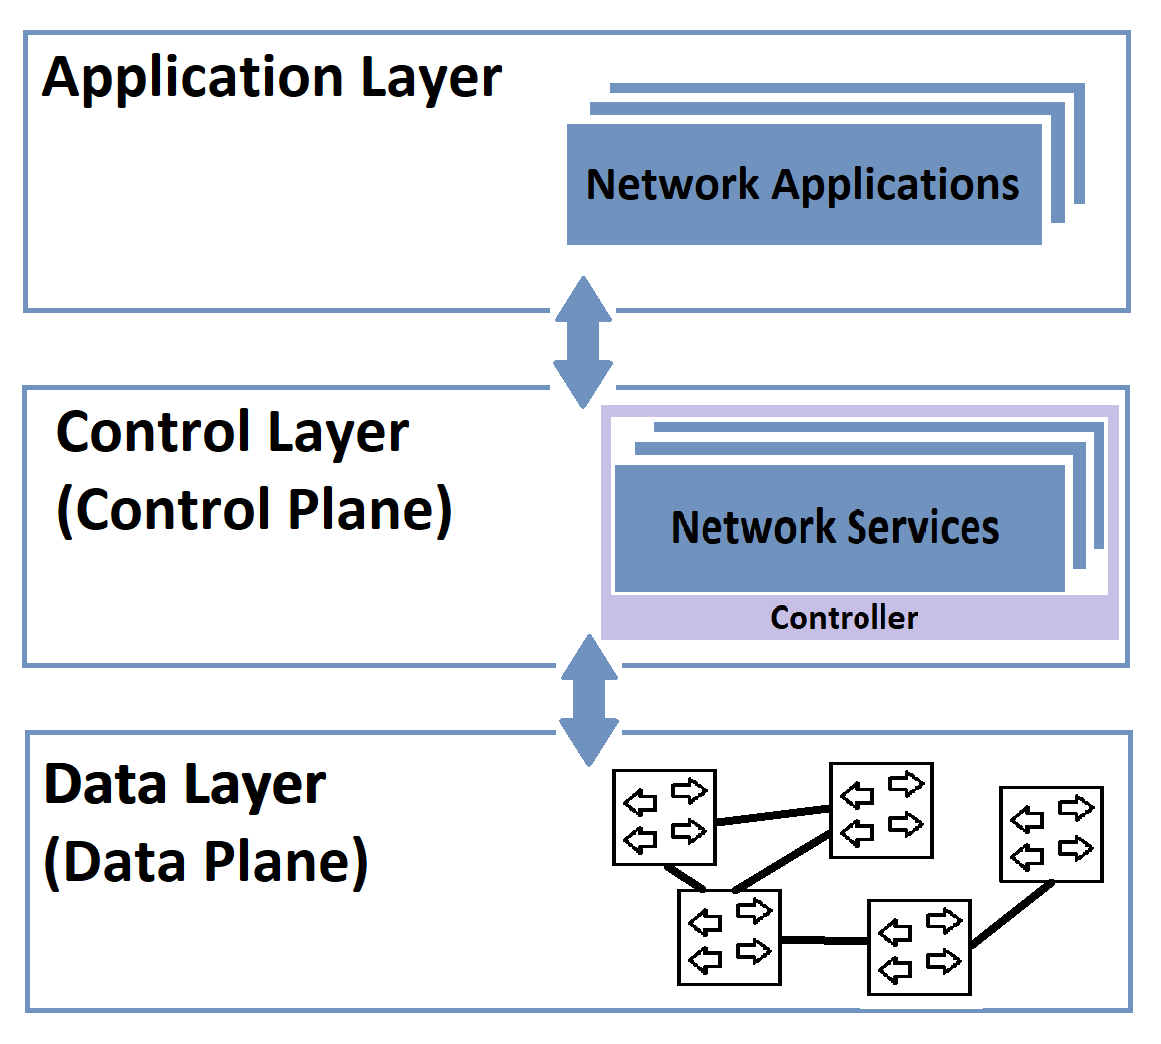
\includegraphics[width=0.4\textwidth]{Bilder/layer2}
	\caption{SDN Architektur}
	\label{layer2}
\end{wrapfigure}
Software-defined Networking beschreibt einen agilen Ansatz zur Verwaltung und Administrierung von Computernetzwerken aus einer zentralen Stelle. Dabei muss nur an der zentralen Stelle eine Änderung vorgenommen werden, um Änderungen an mehrere Netzwerkkomponenten beziehungsweise -bereichen vorzunehmen. Ein sogenannter Controller stellt eine zentrale Stelle dar und steuert den ihm zugehörigen Netzwerkabschnitt. Switches und Routern leiten Pakete nach Regeln beziehungsweise Tabellen weiter, wo üblicherweise für eine Änderung der Regeln jedes Gerät einzeln angesprochen werden muss. Durch die Software im Controller werden Änderungen angenommen und auf die Netzwerkkomponenten übertragen. Diese Vorgehensweise durch Software-defined Networking erlaubt eine dynamische Anpassung des Computernetzwerkes \cite[1-2]{sdn1}.\par 
Durch das Hinzufügen eines Controllers wird die sogenannte Control Plane vom Switch und Router entbunden. Dadurch verbleiben der Switch und der Router in der Data Plane, wo sie weiterhin für die Paketweiterleitung zuständig bleiben. Der Controller hingegen ist nun für die Entscheidungen verantwortlich, wie mit einem Paket verfahren werden soll. Aus der Entkopplung der Control Plane von der Data Plane ergibt sich im Ganzen die sogenannte Application Layer, die Data Plane und dazwischen die Control Plane, was nun Änderungen leichter zulässt (siehe Abbildung \ref{layer2}). Programme können über die application programming interface (API) mit dem Controller kommunizieren und ihm Anweisungen über Pakete oder Netzwerkbereiche geben. Der Controller wiederum wendet die getroffenen Entscheidungen an den zugehörigen Netzwerkkomponenten an \cite[2]{sdn2}. Des Weiteren kann über die API verschiedene Netzwerkleistungen implementiert werden. Darunter zählen neben der Kontrolle des Paketflusses beispielsweise Implementierungen bezüglich der Sicherheit, der Quality of Service (QoS), der Zugriffskontrolle und weitere Leistungen, die für ein Netzwerk wichtig sind \cite[8-9]{sdn2}. \par
Bei klassischen Switches werden anhand eingehender Pakete MAC-Adressen mit dem dazugehörigen Ausgangsport in einer Tabelle hinterlegt. Fehlt diese Information, wird ein Paket auf allen verfügbaren Ports ausgegeben. Hierbei würde ein Switch keine Auslastungen außerhalb seines Bereiches kennen. Aus diesem Grund würde der Switch das Paket auf die für das Ziel vorgesehene Strecke einordnen, die er vorher per Address Resolution Protocol Anfrage (ARP) in seinem Cache abgelegt hat. Der Controller jedoch hat einen Überblick auf das ganze Netzwerk, die von ihm verwaltet wird, weshalb er eine performantere Entscheidung treffen kann, wohin das Paket am besten weitergeleitet werden sollte, um beispielsweise Überlastungen zu vermeiden \cite[1-2]{sdn1}. \par
Über ein im Vergleich zu Hypertext Transfer Protocol (HTTP) junges Protokoll namens OpenFlow (OF) kommuniziert der Controller mit bestimmten Netzwerkkomponenten wie beispielsweise ein OpenFlow Switch, um diese zu steuern. Es gibt zwei Arten von OpenFlow Switches: OpenFlow-only und OpenFlow-enabled Switches. OpenFlow-enabled Switches sind klassische Switches, die zusätzlich OpenFlow fähig sind. OpenFlow-only Switches haben keine zusätzlichen Module eingebaut, auf die Sie zurückgreifen können und müssen deswegen an einen Controller gebunden sein, der dann beispielsweise entscheidet, wohin eingehenden Pakete weiterleitet werden sollen. Dafür sendet der Switch ein Paket oder ein Teil eines Paketes an den Controller und wartet auf einen Befehl, wie er sich zu verhalten hat. Falls der Switch vorher einen Eintrag über das Paket besitzt, greift er auf diese zurück, und wenn überhaupt kein Eintrag vorhanden ist, wird das Paket nach den Einstellungen der Switch entweder verworfen, an allen Ports ausgegeben oder an den Controller gesendet. Die Fähigkeit, bestimmte Befehle auf Pakete anzuwenden, die auf einer Übereinstimmung basieren, zeichnet Software-defined Networking aus \cite[9-10]{sdn2}. \par
Der Controller stellt einen sogenannten Single Point of Failure dar. Das bedeutet, wenn der Controller ausfällt, fallen alle vom Controller abhängigen Netzwerkkomponenten ebenfalls aus. So würde beispielsweise bei einer Denial-of-Service-Attacke durch das Überfluten des Controllers ein Zustand erfolgen, bei dem der Controller an Bandbreite, Speicher und Rechenleistung verlieren und im schlimmsten Fall auch lahmgelegt werden kann. Das ist eines der schlimmsten Szenarien und könnte durch das Hinzufügen eines zweiten Controllers kompensiert werden \cite[3]{sdn3}.

\newpage
\section*{Einleitung von Naghmeh}\label{einl-naghmeh}
In Kommunikationsnetzwerke werden immer größer und komplexer und traditionelle Infrastrukturen, Netzwerksysteme können kaum eine Lösung bitten, um die heutigen Netzwerkanforderungen angemessen zu erfüllen. Dies hat zu einem anderen Ansatz für die Netzwerksystemarchitektur geführt, der als Software defined Networking (SDN) bekannt ist. SDN-Ansätze wurden bereits Mitte der 1990er Jahre eingeführt, sind aber erst seit letzten Jahren ein etablierter Industriestandard geworden. Viele Netzwerkarchitekturen und -systeme haben SDN eingeführt, und Anbieter entscheiden sich für SDN als eine bessere Alternative zu festen und unflexiblen Protokollstapeln. SDN ist eine moderne Netzwerkarchitektur, die die Netzwerksteuerung von Datenübertragungsgeräten entkoppelt und die Netzwerkprogrammierung unterstützt \cite{gelberger2013performance}.\par
SDN trennt die Netzarchitekturen in drei verschiedene Ebenen: Daten-, Kontroll- und Anwendungsebene. Die Datenebene umfasst alle Routing-Geräte, die Weiterleitungsregeln speichern, um den Datenverkehr zu verarbeiten. Die Steuerungsebene besteht aus einem oder mehreren Controllern. Controller ist dafür verantwortlich, den Datenverkehr zu überprüft, Entscheidungen zu treffen und die Netzwerkkonfiguration zu ändert. Der Controller kann auch die Ressourcen optimieren und die Fehlerbehebungsverfahren implementieren. Die Anwendungsebene gruppiert Anwendungen und verarbeitet die Daten für den Controller. SDN definiert auch Schnittstellen für die Kommunikation zwischen Ebenen: Anwendungs- und Steuerungsebene kommunizieren über die Northbound API, und Daten- und Steuerungsebenen verwenden die Southbound-API \cite{rastogi2016comparative}.\par
Die SDN- Architektur hängt stark von der Effizienz der Steuerebene ab, auf der sich der SDN-Controller befindet. Um die Steuerebene möglichst effizient zu gestalten, hat Auswahl des Controllers eine große Bedeutung. Der Controller soll  sowohl weniger Zeit benötigen, um Entscheidungen zu treffen und Entscheidungen an die Datenebene weitergeben, als auch die Herausforderungen des modernen Netzwerkverkehrs bewältigen\cite{rastogi2016comparative}.\par
Das von SDN eingeführte modulare Konzept und die moderne Schichtenstruktur ermöglichen jeder Schicht, unabhängig voneinander zu innovieren, was den Herstellern von Netzwerkgeräten neue Möglichkeiten eröffnet, moderne Netzwerkdienste und -anwendungen zu entwickeln. Netzwerkadministratoren können die Netzwerkleistung und das Netzwerkverhalten in Echtzeit überwachen. Sie können auch Entscheidungen über die Bereitstellung von Netzwerkdiensten oder Änderungen der Topologie und Konfiguration von ihrem Arbeitsplatz treffen und diese durchzuführen \cite{hasan2020sdn}.\par
SDN eignet sich auch ideal für die Entwicklung von Mechanismen zur Bewältigung von Sicherheitsproblemen, aber dazu müssen die Administratoren die Controller für die Ausführung bestimmter Aufgaben erweitern. Diese Art von Mechanismus kann auf der Steuerungsebene oder als eine Reihe von Teilen auf der Anwendungs- und Steuerungsebene ausgeführt werden \cite{morales2015extending}.\par
Die wichtigste Funktion, die SDN für Computernetzwerke bietet, ist die Möglichkeit, das Netzwerk zu programmieren und es flexibler und einfacher zu verwalten. Diese Fähigkeit spielt eine wichtige Rolle bei der Reduzierung des Gesamtsystemkapitals und der Verwaltungskosten sowie bei der Verbesserung von Leistung, Zuverlässigkeit und Servicequalität. Die ständige Nachfrage nach Neukonfiguration bestehender Netzwerke aufgrund von Bandbreite und neuen Technologien (Hard- und Software) ist sehr anspruchsvoll und komplex. Mit der SDN-Technologie wird dieser Prozess im Vergleich zu herkömmlichen Netzwerken vereinfacht\cite{hasan2020sdn}.

\newpage
\section*{Einleitung von Tung}\label{einl-tung}
Derzeit gibt es viele Definitionen von SDN, aber laut ONF (Open Networking Foundation – eine gemeinnützige Organisation, die die Entwicklung von SDN durch das Studium geeigneter offener Standards unterstützt), ist SDN definiert als: „Software-Defined Networking (SDN) ist eine aufstrebende Architektur, die dynamisch, verwaltbar, kostengünstig und anpassungsfähig ist, wodurch sie sich ideal für die hohe Bandbreite und Dynamik heutiger Anwendungen eignet. Diese Architektur entkoppelt die Netzwerksteuerungs- und Weiterleitungsfunktionen, wodurch die Netzwerksteuerung direkt programmierbar und die zugrunde liegende Infrastruktur für Anwendungen und Netzwerkdienste abstrahiert werden kann.”\cite{ONFTung} Diese Definition kann sehr allgemein und verwirrend sein. Um zu verstehen, was SDN ist, erinnern wir uns zunächst ein wenig an die traditionelle Netzwerkarchitektur.


Andreas Donner beschreibt das herkömmliche Netzwerk: 
Konventionelle Netzwerke bestehen aus Routern und Switches, die mit proprietärer, herstellerspezifischer      Firmware betrieben werden. Die Datenpakete werden von den Komponenten gemäß den Vorgaben der Software weitergeleitet. Die Netzwerkgeräte besitzen intern spezielle Hardware, die für die Weiterleitung der Pakete verantwortlich ist. Die Steuerung der Hardware übernimmt die Software und Kontrollebene des Betriebssystems, das ebenfalls auf dem Gerät integriert ist. \cite{tranetworkTung}
Es bedeutet, jedes Gerät im Netzwerk verfügt sowohl eine logische Rolle in der Steuerleitung als auch die Weiterleitung von Datenpakete. Im traditionellen Netzwerk, der Administrator muss bei der Konfiguration eines Mehrkomponentennetzwerks jedes Gerät manuell konfigurieren, und die Geräte sind in Bezug auf die Verwaltung nicht miteinander verbunden. Daher ist es besonders schwierig zu konfigurieren und zu bedienen. Die Geräte sind völlig unabhängig, sodass die Konfiguration an jedem Gerät nur manuell nacheinander geändert werden kann.

Die SDN-Architektur hat drei Ebene, die über Northbound- und Southbound\hyp{}Anwendungsprogrammierschnittstellen (APIs) kommunizieren. Die Ebene umfassen:
\begin{itemize}
	\item Application Plane – SDN-Anwendungen kommunizieren Verhalten und benötigte Ressourcen mit dem SDN-Controller.
	\item Control Plane – Verwaltet Richtlinien und Verkehrsfluss. Der zentralisierte Controller verwaltet das Verhalten der Datenebene.
	\item Data Plane – Besteht aus den physischen Switches im Netzwerk.\cite{SDNdefTung}
\end{itemize}



Mit der obigen Architektur bietet SDN verschiedene Möglichkeiten. Die Control Plane kann direkt programmiert werden. Das Netzwerk wird durch Änderungen auf der Control Plane schnell angepasst und geändert. Das Netzwerk wird zentral verwaltet, da die Steuerung auf der Control Plane zentralisiert ist. Die Konfigurationen der Data Plane können auf der Application Plane programmiert und an die unteren Schichten kommuniziert werden.

Netzwerkgeräte haben nur die Funktion, Daten weiterzuleiten, und der Routing-Teil wurde auf ein anderes Gerät übertragen, das als Controller für das gesamte Netzwerk fungiert und als SDN-Controller bezeichnet wird. Es enthält alle Routing-Algorithmen, Safety-, Security- und Load-Balancing-Lösungen. Bei der Konfiguration des gesamten Netzwerks muss der Administrator nur die Algorithmen auf diesem Gerät mit Software schreiben und ändern, alle Netzwerkgeräte werden synchron verwaltet. Wenn Benutzer Parameter oder Anforderungen für das Netzwerk ändern möchten, ändern sie diese einfach in der Verwaltungssoftware des SDN-Controllers. Dies ist völlig anders als herkömmliche Netzwerktechnologie \cite[37-38]{ 6553676}


Mit SDN kann der Administrator des Netzwerks alle Switching-Regeln des Netzwerks nach Bedarf ändern. Administratoren können bestimmte Pakettypen mit einem bestimmten Maß an Kontrolle und Sicherheit priorisieren, depriorisieren oder sogar blockieren. Dies ist besonders nützlich in Cloud-Computing-Architekturen, da es Administratoren ermöglicht, den Datenverkehr flexibler und effizienter zu verwalten, wenn es mehrere Dienstmandanten gibt. Im Wesentlichen ermöglicht dies Administratoren, Switches effizienter zu nutzen und mehr Kontrolle über den Netzwerkverkehr zu haben als je zuvor. \cite{cloudcomputing}


Weitere Vorteile von SDN sind, dass es Verwaltung und Einblick in die Komponenten und Konfiguration des Netzwerks bietet. Administratoren müssen nur mit einem einzigen zentralen Controller interagieren, um Richtlinien an verbundene Switches im Netzwerk zu verteilen, anstatt mehrere Geräte einzeln konfigurieren zu müssen. Diese Fähigkeit ist auch in Bezug auf die Sicherheit ein großer Vorteil, da der Controller den Datenverkehr überwachen und Sicherheitsrichtlinien zentral, synchron und einfach implementieren kann. Wenn der Controller beispielsweise verdächtigen Datenverkehr sieht, kann er das Paket sofort umleiten oder verwerfen, ohne es an einen anderen Handler weiterzuleiten.\cite{sdnbenefitstung}


\newpage
\section{Motivation}
{\tiny Verfasst von: James\par}
Das Modul “Informatik Projekt” wird im 5. Semester des Bachelorstudiengangs Informatik durchgeführt. Nach erfolgreichem Abschluss des Moduls sollten Studierende gewisse Kompetenzen erlernt haben, wie beispielsweise den Software-Engineering Prozess planen und durchführen, als auch auf einem vertieften Niveau gemeinsam programmieren zu können. Außerdem sollten Studierende fähig sein, gemeinsam ein Team zu bilden und einen selbsterstellten Zeitplan einzuhalten sowie auf einem technisch hohen Niveau zu kommunizieren, um als Team auf Ergebnisse zu kommen. Falls unerwartete Komplikationen sowohl technischer als auch sozialer Art entstehen, sollte als Team diese Hürde überwunden werden. Infolgedessen entstand dieser Projektbericht, der als Projektergebnis und als Dokumentation dient, um die erlernten Kompetenzen widerzuspiegeln.\par
Durch das Thema “Software-Defined Networking mit Openflow” konnte Freizeit mit Studium verbunden werden, da viele selbsterlernte Kenntnisse und Vorkenntnisse aus anderen Modulen praktisch angewendet werden konnten. Zugleich dient die Dokumentation durch ausführliche Erklärungen und Abbildungen auch als Tutorial, dass den Einstieg in das Thema SDN durch Praxis vereinfachen soll.
\section{Problemstellung}
{\tiny Verfasst von: James\par}
Innerhalb des Informatikprojekts muss sich folgendes Szenario vorgestellt werden:\par
Ein Unternehmen plane eine Netzwerkkommunikation zwischen vier Standorten mittels Sofware-Defined Networking Funktionen. Die Hauptverwaltung befinde sich in Frankfurt am Main, die drei weiteren Niederlassungen seien in München, Berlin, Hamburg. Zudem sollte jede Lokation einen Asymmetric Digital Subscriber Line Zugang (ADSL) zum Internet haben.\par
Darüber hinaus müssen im Netzwerk bestimmte Funktionen und Aufgaben realisiert werden. Es solle nicht nur für jede Lokation jeweils ein privater IP-Adressenbereich genutzt werden, sondern auch ein Netzwerkplan vom gesamten Netzwerk erstellt werden. Außerdem solle jede Kommunikation zwischen den einzelnen Lokationen über eine Virtual Private Network Verbindung (VPN) laufen, somit sei der gesamte Datenverkehr über das Internet und zwischen den Lokationen verschlüsselt. Anschließend müsse ein Service-Provider gefunden werden, der die gewünschte Konfiguration und Anforderungen realisiere. Jedoch sollen der Preis und die benötigte Bandbreite nicht nur für den Internetzugang, sondern auch für die Wide Area Network-Verbindungen (WAN) beachtet und verglichen werden. Ebenfalls solle durch SDN sowohl eine Network Address Translation-Firewall-Funktion (NAT) als auch eine Webproxy-Funktion in allen Lokationen implementiert werden. Ergänzend dazu solle mithilfe des SDN-Controllers sowohl eine graphische Darstellung der Netzwerkstruktur durch einen Topologieviewer realisiert werden als auch eine Monitoring-Lösung. Zudem müsse eine Quality of Service -Funktion implementiert werden, die genügend Bandbreite für Audio beziehungsweise (bzw.) Video-Konferenzen habe, auch wenn diese über die WAN-Verbindung mit Symmetric Digital Subscriber Line (SDSL) 20 Megabit begrenzt sei. Anschließend wird ein weiteres Szenario beschrieben:\par
“Für eine Spezialanwendung muss eine Software in Berlin wichtige Daten an einem Server in der Zentrale senden, dazu kann diese Software über die API mit dem Controller kommunizieren und diesem dies mitteilen. Dadurch wird der Controller nun alle Knoten auf diesem Weg durchs Netzwerk anweisen, diesen Flow zu priorisieren und alle anderen Datenströme zu drosseln.” 
Schließlich sollen die Netzwerkfunktionen Hub (Repeater), Bridge, Layer-2-Switch, Layer-3-Switch, Dynamic Host Configuration Protocol (DHCP) und Domain Name System (DNS) analysiert und realisiert werden.\par
In Kapitel 3 wird für die Implementierungen der Netzwerk Funktionalitäten Screenshots von Mininet in VirtualBox gezeigt, die als Nachweis der einzelnen Funktionalitäten dienen sollen.


\section{Aufbau der Arbeit}
{\tiny Verfasst von: James\par}
In Kapitel 2 dieser Projektarbeit wird über das generelle Vorgehen in dem Projekt geschrieben. Nach einer kurzen Vorstellung unseres Projektziels, wird das konkrete Vorgehen innerhalb der Gruppe erläutert. Weiterhin wird sowohl über die Festlegung der Meilensteine, als auch über die genutzten Werkzeuge eingegangen. In Kapitel 3 wird die Projektdurchführung erklärt und in den Unterkapiteln werden die erreichten Ergebnisse vorgestellt, die auch die einzelnen Thematiken der jeweiligen Funktionalitäten ergänzen. Anschließend dient Kapitel 4 mit einer kurzen Analyse aller Ergebnisse, als auch eine kritische Betrachtung der Projektanforderung, als Auswertung und Selbstreflektion, was im Rahmen der Projektarbeit nicht funktionierte und umgesetzt werden konnte, in Bezug auf Netzwerkanforderungen, sowie intern zwischen allen Gruppenmitgliedern. Kapitel 5 bildet mit dem Fazit einen Ausblick in die mögliche Zukunft für SDN.


\chapter{Projekt}
\section{Projektziel}
{\tiny Verfasst von: Tung\par}
Ziel des Projekts war es, ein Netzwerk für ein Unternehmen mit vier Lokationen aufzubauen. Dabei war es besonders wichtig, dass das gesamte Netzwerk mit SDN Funktionen realisiert wurde.\par
Ein stabiles Netzwerk vom ersten Tag an wird die Grundlage für den Erfolg von Unternehmen sein. Damit Unternehmen gut funktionieren, muss auch das Netzwerksystem gut funktionieren. Das Netzwerk arbeitet mit der richtigen Kapazität und bringt Effizienz. Die Aufgabe war es, ein gutes stabiles Netzwerk aufzubauen, dass zu 100 Prozent bei Datenverkehr funktionierte und unerwartete Sicherheitsprobleme vermeidete.\par
Das Netzwerksystem musste eng verwaltet und überwacht werden. Zudem musste es leicht unterstützt werden, um Probleme auf die effektivste Weise behandeln und beheben zu können. Es war zwingend erforderlich, dass das Netzwerksystem sicher und verschlüsselt war. Denn Unternehmensdaten sind das Wichtigste. Bei der Netzwerksicherheit ging es auch um den Schutz von Unternehmensressourcen. Je nach Verwendungszweck und Anzahl der Nutzer sollten genügend Bandbreite zur Verfügung gestellt werden.\par
Im Laufe des Projektberichtes werden die erfolgreichen sowie erfolglosen Ergebnisse des Projekts dokumentiert und dargestellt. Am Ende des Projektes wird ein lauffähiges Produkt entstehen, dass alle benötigten Funktionalitäten erfüllt.  

\section{Vorgehen}
{\tiny Verfasst von: Tung\par}
Angemessene Aufgabenverteilung im Kollektiv, brachte viele Vorteile für die Arbeitssituation und den Teammitgliedern. Die Nutzung der maximalen Kapazität jedes Teammitglieds war ein effektiver Weg, um die Arbeitseffizienz zu verbessern.\par
Um die Wünsche und Fähigkeiten jedes einzelnen Mitglieds zu verstehen, wurden Gespräche und Diskussionen frühzeitig durchgeführt. Die Zuweisung von Aufgaben, die der Produktivität jeder Person entsprachen, half den Mitgliedern, effektiver und mit einem angenehmeren Geist zu arbeiten. Den Mitgliedern wurden bestimmte Aufgaben mit Fristen zugewiesen. Es wurde jede Woche ein permanentes Treffen über Discord gehalten. Spontane Treffen konnten mit dem höchsten Geist und der höchsten Konzentration ebenfalls durchgeführt werden.\par
Die Analyse von Aufgabenzuweisungen war wichtig, um zu verstehen, was getan werden muss und welche Tools notwendig seien. Der Wissensaustausch half den Mitgliedern, sich Wissen sofort anzueignen und effektiv zu nutzen. Nach einer erfolgreichen Analyse begann unser Team mit der Ausarbeitung eines Plans. Die Arbeit wurde vom Projektleiter aufgeteilt und kontrolliert.

\section{Festlegen von Meilensteinen}
{\tiny Verfasst von: Tung, Naghmeh, James, Mücahit\par}
In dem ersten Treffen der Gruppe wurde entschieden, drei zentrale Meilensteine zu definieren (siehe Abbildung \ref{milestones}). Grund dafür sei, einen klaren Faden in der Projektarbeit zu konstruieren, um mit der Menge an Informationen strukturiert umgehen zu können. Die Meilensteine wurden mithilfe der Aufgabenstellungen konkretisiert:

\begin{figure}[H]
 \centering
 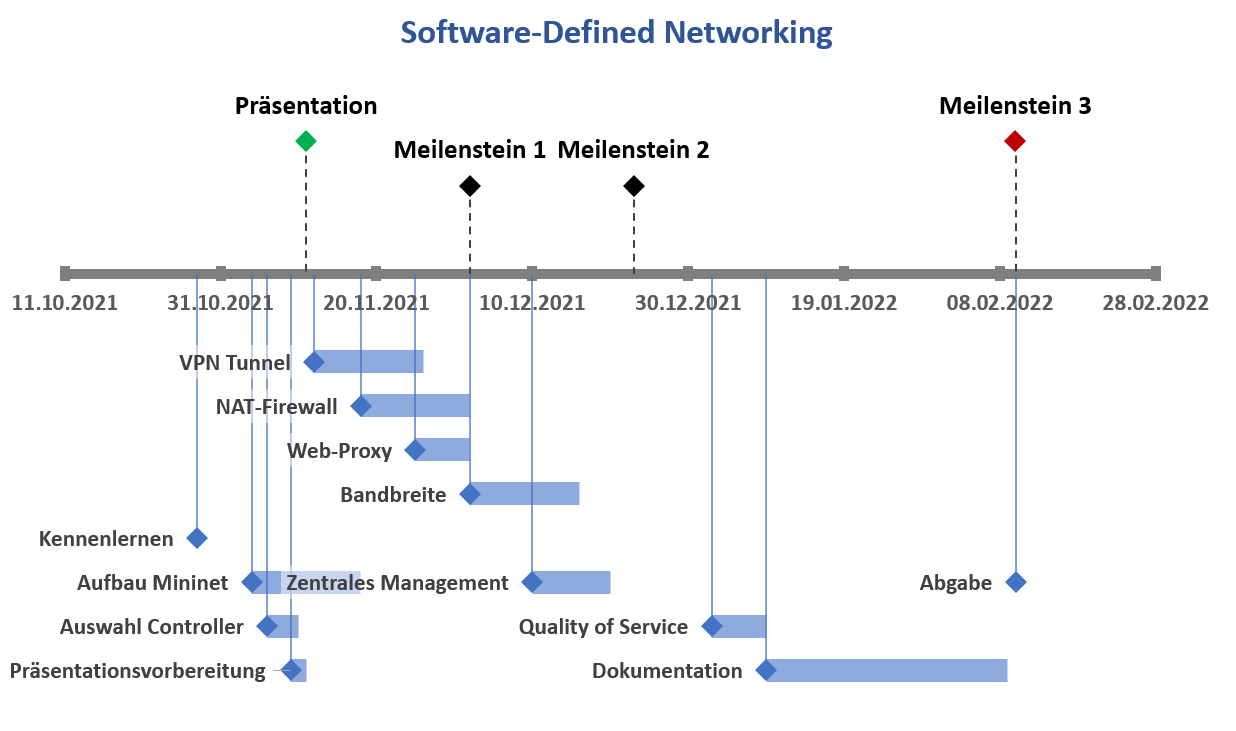
\includegraphics[width=1.0\textwidth]{Bilder/meilensteine}
 \captionsetup{justification=centering,margin=2cm}
 \caption{Zeitplan des Projektes}
 \label{milestones}
\end{figure}

\textbf{Meilenstein 1}
\begin{itemize}
 \item Erstellung eines Netzwerkplans für das gesamte Netzwerk
 \item Kommunikation zwischen Lokationen soll über eine VPN Verbindung realisiert werden
 \item Produktauswahl bei einem ISP zur Realisierung des Netzwerkes
 \item Implementierung einer NAT-Firewall-Funktion in allen Lokationen
 \item Deadline: 02.12.2021
\end{itemize}

\textbf{Meilenstein 2}
\begin{itemize}
 \item Implementierung einer Webproxy-Funktion für den Internet-Zugang in den einzelnen Lokationen
 \item Implementierung eines Topologie-Viewers und einer Monitoring-Lösung
 \item Implementierung einer Quality of Service Funktion für Audio- und Videokonferenzen
 \item Deadline: 23.12.2021
\end{itemize}

\textbf{Meilenstein 3}
\begin{itemize}
 \item Priorisierung von einem Datenflow mithilfe des Controllers
 \item Analyse und Umsetzung der Netzwerkfunktionen von Hub, Bridge, Layer-2-Switch, Layer-3-Switch, DHCP und DNS
 \item Deadline: 10.02.2022
\end{itemize}

Durch gängige IT-Projektmanagementmethoden, wie beispielsweise die Scrum-Methode, konnten frühzeitig Ergebnisse erzielt werden. Infolgedessen gab es am Ende der Projektarbeit mehr Zeit, um über Kleinigkeiten zu reflektieren.

\section{Verwendete Werkzeuge}
{\tiny Verfasst von: Naghmeh\par}
Im Folgenden werden die für die Implementierung und Evaluierung verwendeten Hardware- und Softwareumgebungen kurz beschrieben.\par
Dieses Projekt wurde auf VirtualBox Oracle VM Version 6.1 durchgeführt. Unter der Verwaltung von VirtualBox wurde Mininet-Emulator Version 2.3 und Floodlight Controller Version 1.2 installiert. Zur Ausführung von Programmen zur Evaluation wurde außerdem Python3 installiert. Weitere Programme sind auch installiert und sie werden im Ablauf von Kapitel 3 bekannt gegeben und ausführlicher erklärt.

\subsection{Mininet}
{\tiny Verfasst von: Tung\par}
Der Mininet-Emulator implementiert die Verbindung zwischen Switches und Controllern. Diese ermöglicht es Entwicklern, die an der Erstellung und dem Testen von Controller-Ressourcen interessiert sind, Mininet zur Durchführung ihrer Simulationen zu nutzen \cite{mininetoverview}.

\subsubsection{Einführung}
{\tiny Verfasst von: Tung\par}
Mininet ist ein Netzwerk Emulator, mit der Netzwerke simuliert werden können. Bei Mininet handelt es sich um eine kostenlose Open-Source-Software, die die virtuelle Maschine und dem Controller die Recherche in SDN und OpenFlow ermöglicht. Mininet ermöglicht eine sehr groß angelegte Topologie, wodurch ein Netzwerk von Hosts, Switches, virtuellen Links und einem Controller erstellt wird \cite[139]{mininetdefinition}. Das Ausführen von Tests mit den Komponenten ist unkompliziert und kann über Python-Schnittstelle erledigt werden. Benutzer können ihre eigene Netzwerktopologie-Struktur nach ihren eigenen Bedürfnissen aufbauen\cite[141]{mininetdefinition}.

\subsubsection{Funktionalität}
{\tiny Verfasst von: Tung\par}
Mininet:
\begin{itemize}
 \item stellt ein einfaches Netzwerk Testbed dar, welches aber auch gleichzeitig günstig ist. Da der OpenFlow Switch in Mininet alle Eigenschaften wie ein echter OpenFlow Switch hat, ist die Anwendung von einem Netzwerkemulator mit Mininet praktisch sinnvoll.
 \item ermöglicht das Debuggen und Ausführen von Tests größerer Netzwerke mithilfe von Command Line Interface (CLI).
 \item unterstützt das Einrichten beliebiger benutzerdefinierter Diagramme. Die Anwendungen im Mininet können im echten Netzwerk realisiert werden, ohne dass der Code geändert werden muss.
 \item bietet eine benutzerfreundliche und erweiterbare Python-API.
 \item ermöglicht mehreren gleichzeitigen Entwicklern, unabhängig voneinander an derselben Topologie zu arbeiten.
 \item ermöglicht komplexe Topologietests, ohne dass ein physisches Netzwerk verkabelt werden muss \cite{mininetoverview}.
\end{itemize}

\subsubsection{Nachteile}
{\tiny Verfasst von: Tung\par}
Aktuell ist Mininet nur unter Linux lauffähig. Nutzer eines anderen Betriebssystems müssen auf Linux entweder durch Simulierung oder Installation zurückgreifen. Zudem könnte der Sourcecode effizienter und sauberer implementiert werden.\par
Mininet schreibt Ihren OpenFlow-Controller nicht für Benutzer. Wenn Benutzer benutzerdefiniertes Routing- oder Schaltverhalten benötigen, müssen Benutzer einen Controller mit den erforderlichen Funktionen finden oder entwickeln.\par
Standardmäßig ist Mininet-Netzwerk von Local Area Network (LAN) und vom Internet isoliert - das ist normalerweise eine gute Sache! Benutzer können jedoch das NAT-Objekt und/oder die Option --nat verwenden, um Ihr Mininet-Netzwerk über Network Address Translation mit Ihrem LAN zu verbinden. Benutzer können Ihrem Mininet-Netzwerk auch eine echte (oder virtuelle) Hardware-Schnittstelle hinzufügen (siehe Beispiele/hwintf.py für Details).\par
Standardmäßig teilen sich alle Mininet-Hosts das Host-Dateisystem und den PID\hyp{}Speicherplatz. Das bedeutet, dass Benutzer möglicherweise vorsichtig sein müssen, wenn sie Daemons ausführen, die eine Konfiguration in /etc erfordern, und Benutzer müssen darauf achten, dass sie nicht versehentlich die falschen Prozesse beenden. \par
Im Gegensatz zu einem Simulator hat Mininet keine starke Vorstellung von virtueller Zeit. dies bedeutet, dass Timing-Messungen auf Echtzeit basieren und dass Ergebnisse schneller als Echtzeit (z. B. 100-Gbit/s-Netzwerke) nicht einfach emuliert werden können \cite{mnnachteile}.

\subsubsection{Komponenten}
{\tiny Verfasst von: Tung, Naghmeh, James, Mücahit\par}
Ein Mininet-Netzwerk besteht aus den folgenden Komponenten:
\begin{itemize}
 \item \textbf{Link:} Links sind virtuelle Ethernets, die zwei virtuelle Schnittstellen verbinden. Jeder Link verhält sich für das gesamte System wie ein echter funktionsfähiger Ethernet-Anschluss. Die Datenrate jedes Links wird von Linux Traffic Control (TC) festgelegt.
 \item \textbf{Hosts:} Ein emulierter Host ist eine Reihe von Prozessen auf Benutzerebene, die in einen Netzwerk-Namespace verlagert wird. Netzwerk-Namespaces bieten Prozessgruppen privaten Besitz von Schnittstellen, Ports und Routing-Tabellen.
 \item \textbf{Switch:} Mininet verwendet Open vSwitches, die im Kernelmodus ausgeführt werden, um Pakete zwischen verschiedenen virtuellen Netzwerkschnittstellen auszutauschen. Open vSwitches sind OpenFlow-fähig und bieten die gleiche Semantik für das Senden von Paketen wie einen realen Switch.
 \item \textbf{Controller:} Ein Controller ist in der Mininet-Simulation ein Knoten, der einen OpenFlow-Controller darstellt. Mininet bietet die Möglichkeit einen internen oder externer Controller zu benutzten. Für den externen Controller wird die IPv4-Adresse und der Port benötigt.
\end{itemize}


\subsubsection{Installation}
{\tiny Verfasst von: Tung\par}
Mininet kann auf verschiedene Weisen installiert werden. In unserer Arbeit wurde die Option: Native Installation from Source ausgewählt. Die Installation wird Schritt für Schritt aufgeführt \cite{mnapi}:
\begin{itemize}
\item[1.] Git wird über das Linux-Terminal installiert
\end{itemize}
\colorbox{CadetBlue}{\textcolor{white}{\textbf{\textsf{\$ sudo apt-get install git}}}}
\begin{itemize}
\item[2.] Über das git Kommando wird die aktuellste Version von Mininet installiert
\end{itemize}
\colorbox{CadetBlue}{\textcolor{white}{\textbf{\textsf{\$ git clone git://github.com/mininet/mininet}}}}
\begin{itemize}
\item[3.] Mit install.sh die Installation starten
\end{itemize}
\colorbox{CadetBlue}{\textcolor{white}{\textbf{\textsf{\$ sudo mininet/util/install.sh -a}}}}

\subsubsection{Aufbau}
{\tiny Verfasst von: Tung\par}
Durch die Eingabe von dem Befehl \textit{\textbf{sudo mn}} wird ein Standardnetzwerk mit zwei Hosts, einer Switch und einem Controller gestartet (siehe Abbildung \ref{sudomn}).

\begin{figure}[H]
 \centering
 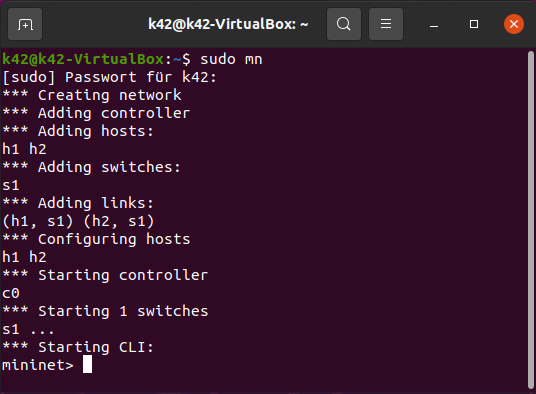
\includegraphics[width=0.5\textwidth]{Bilder/sudomn}
 \captionsetup{justification=centering,margin=2cm}
 \caption{Erstellung eines Standardnetzwerkes mit Mininet}
 \label{sudomn}
\end{figure}

\subsection{Floodlight}
{\tiny Verfasst von: Mücahit, Tung\par}
Floodlight ist ein sogenannter SDN-Controller in der Control Plane. Dieser kommuniziert mit der Data Plane über ein Kommunikationsprotokoll namens OpenFlow und verwaltet diesen \cite[161]{floodlightdefinition}.

\subsubsection{Einführung}
{\tiny Verfasst von: Mücahit, Tung\par}
In den letzten Jahren wurde eine Vielzahl unterschiedlicher SDN-Controller entwickelt. Aus diesem Grund gibt es mittlerweile eine riesige Auswahl an SDN-Controllern für die breit gefächerten Einsatzzwecke, wo unteranderem OpenDaylight, Ryu, POX, NOX und Floodlight dazugehören. Mit allen Controllern sollten alle Projektziele der Projektarbeit erreichbar sein \cite{controllers}.\par
{\tiny Verfasst von: Mücahit\par}
Floodlight wurde als Controller ausgewählt, da einige Punkte und das daraus resultierende Gesamtprodukt die Gruppe überzeugen konnte. Dazu gehört unteranderem die einfache und gut beschriebene Installation. Die moderne Webbenutzeroberfläche und die verständliche, gut dokumentierte REST-API sind sehr benutzerfreundlich und leicht zu verstehen. Daraus resultiert auch die Option, die REST-API über ein Python-Skript zu benutzen. Die Einbindung des Floodlight-Controllers in Eclipse ermöglicht die Implementierung, Untersuchung und das Debuggen verschiedenster Controller-Funktionen. Die gute Dokumentation des in Java geschriebenen Controllers und einige mit der Installation mitgelieferten Module geben dem Entwickler einen guten Start zur Entwicklung von Netzwerkfunktionen.

\subsubsection{Funktionalität}
{\tiny Verfasst von: Mücahit\par}
Die Funktionalitäten des Floodlight-Controllers unterscheiden sich anhand der Ausführung und der Implementierung. Funktionen können über die Webbenutzeroberfläche per Eingabe ausgeführt werden (siehe Abbildung \ref{webui}). Das Einstellen der Firewall und der Access Control List sind zwei dieser Funktionen. Nach Aktivierung der Firewall werden alle Pakete, die nicht in der Liste eingetragen sind, fallen gelassen. Die Access Control List arbeitet ähnlich wie die Firewall, wohingegen nur eine Liste mit erwünschten und nicht erwünschten Quellen existiert. Die Quellen werden anhand der Paket-Informationen angegeben. Bei einem Treffer wird die Quelle je nach Einstellung zugelassen oder verweigert. Folglich verweigert die Firewall jegliche Verbindung nach Aktivierung, wohingegen die Access Control List nur bestimmte Zugriffe auf ein Netzwerk zulässt oder ablehnt \cite{firewall}. \par
Auf der Webbenutzeroberfläche sind Informationen zu dem vom Controller gesteuerten Netzwerk einsehbar. Dazu gehört die Anzahl der Switches, Hosts und Links sowie der verbrauchten Ressourcen des Controllers und der Netzwerktopologie. Die Statistikfunktion des Controllers kann auf der Benutzeroberfläche aktiviert werden. Dieser dient zur ausführlichen Weiterverarbeitung und der Anzeige der vom Controller gesammelten Statistik. Dazu gehören die Flow, meter, queue, aggregate, table und port Statistiken. Die Sammlung benutzerdefinierter Statistiken sind ebenfalls möglich und müssen vom Entwickler nachimplementiert werden. Über die REST-API können sogenannte Flows eingetragen werden, die zur Steuerung des Netzwerkes beitragen. Dabei können Datenpakete modifiziert, zwischengespeichert und umgeleitet werden \cite{statistik}.

\begin{figure}[H]
 \centering
 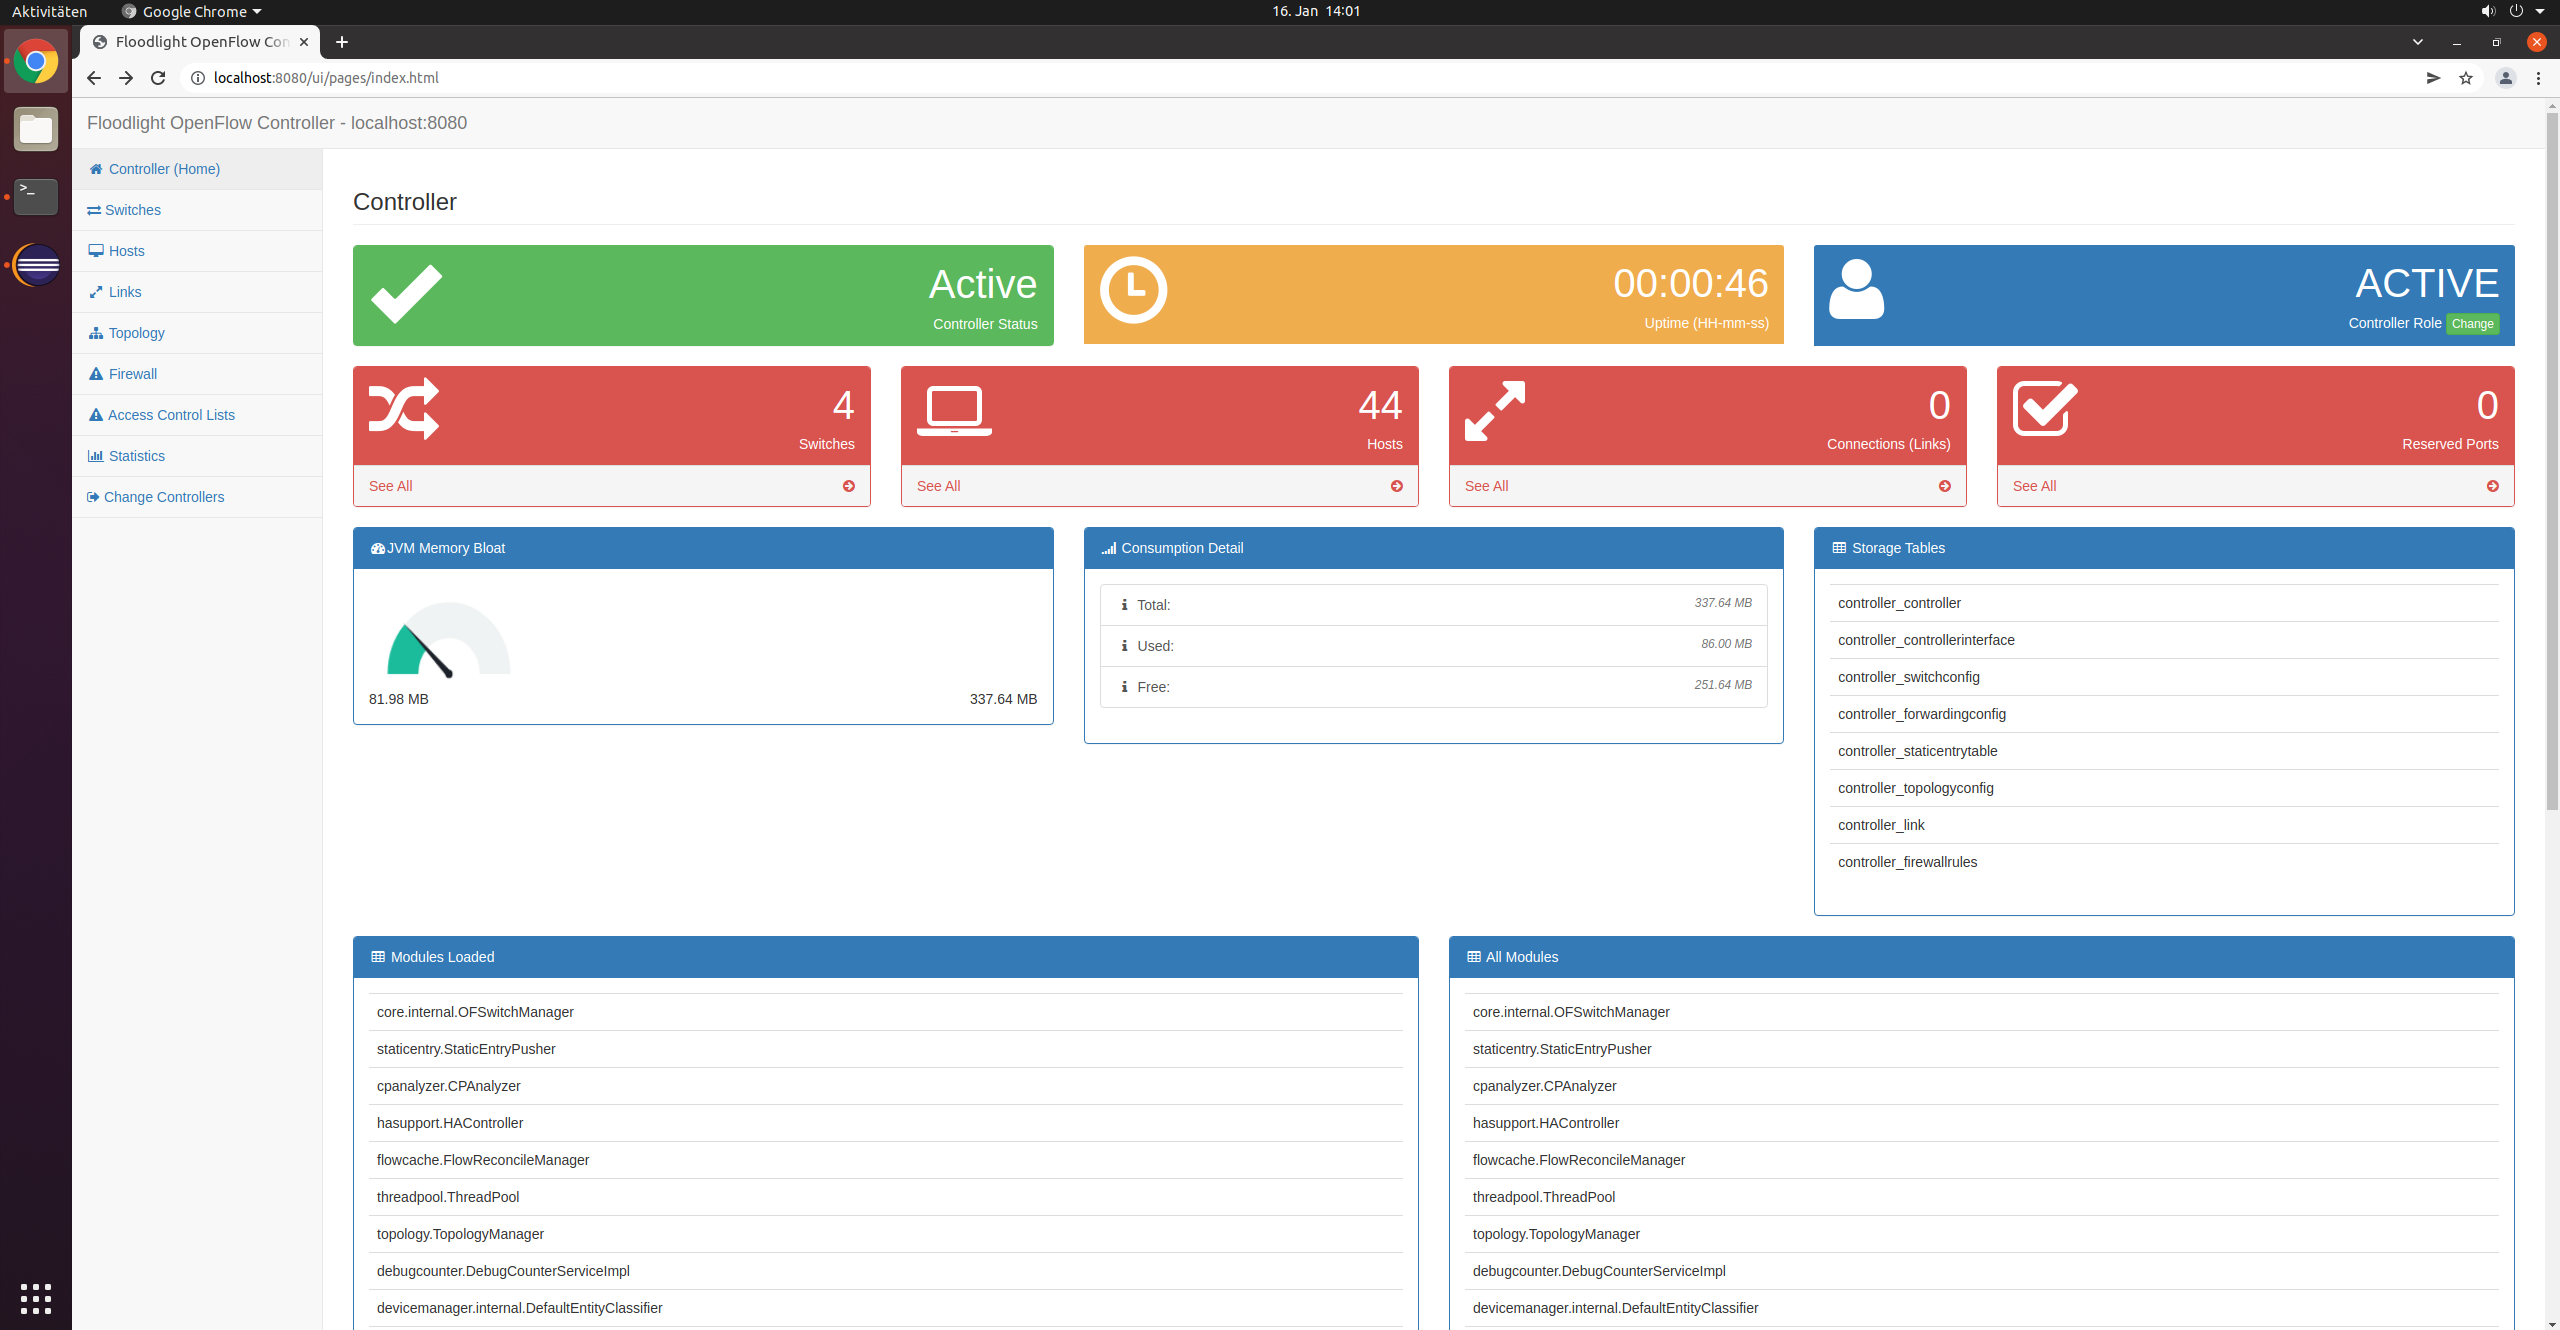
\includegraphics[width=1.0\textwidth]{Bilder/webui}
 \captionsetup{justification=centering}
 \caption{Webbenutzeroberfläche vom Floodlight-Controller}
 \label{webui}
\end{figure}


\subsubsection{Nachteil}
{\tiny Verfasst von: Mücahit\par}
Das ganze Netzwerk ist betroffen, wenn Floodlight ausfällt oder nicht erreichbar ist. Dieser Single Point of Failure gilt für alle Controller und stellt ein Risiko für Netzwerke, die eine hohe Verfügbarkeit und Zuverlässigkeit fordern \cite{failure}.

\subsubsection{Komponenten}
{\tiny Verfasst von: Mücahit\par}
Mit der Installation von Floodlight kommen sogenannte Module zum Einsatz. Die meisten der Module sind bereits aktiviert und stellen bestimmte Funktionen zur Verfügung. Einer davon ist die Learning Switch, welcher für die Speicherung der Routen zu den Hosts zuständig ist. Wenn ein Host einen anderen Host im gleichen Netzwerk erreichen will und der Switch die Route nicht kennt, wird ein Broadcast ausgeführt, der die Anfrage auf allen Ports ausgibt. Wenn der Host antwortet, speichert der Switch die MAC-Adresse des jeweiligen Hosts ab und muss somit keinen Broadcast durchführen \cite{broadcast}. Weitere Beispielmodule wären der Load Balancer, der für einen Ausgleich des Datenverkehrs im gesamten Netzwerk sorgt \cite{loadbalance}. Über die REST-API stellt Floodlight die Netzwerktopologie über die Webbenutzeroberfläche grafisch dar. Es existieren noch weitere Module, wobei auch eigene programmiert werden können \cite{restapi}.

\subsubsection{Installation}
{\tiny Verfasst von: Mücahit\par}
Die Installation des Floodlight-Controllers kann auf den Betriebssystemen Linux, Mac oder Windows erfolgen. Es wird das Java Development Kit 8, Maven, Git, build-essential und das Python Development Paket benötigt. Da Floodlight in Java geschrieben wurde, wird auch zur Ausführung Java verwendet. Maven wird zum sogenannten Builden benutzt, bei dem die Software Floodlight aus mehreren Dateien zusammengestellt wird. Das Python Development Paket wird zur Ausführung und Git zum Herunterladen von Floodlight vorausgesetzt. Build-essential werden zum Kompilieren einiger Software verwendet. Im Folgenden wird die Installation auf Linux Schritt für Schritt erklärt. Befehle müssen im Linux-Terminal zeilenweise eingegeben werden \cite{install}.

\begin{itemize}
\item[1.] Alle benötigten Abhängigkeiten installieren.
\end{itemize}
\colorbox{CadetBlue}{\textcolor{white}{\textbf{\textsf{\$ sudo apt-get install build-essential git maven python-dev openjdk-8-jdk}}}}
\begin{itemize}
\item[2.] Java Compiler als Alternative festlegen. Befehl eingeben und JDK 8 Auswählen.
\end{itemize}
\colorbox{CadetBlue}{\textcolor{white}{\textbf{\textsf{\$ sudo update-alternatives --config javac}}}}
\begin{itemize}
\item[3.] Programmcode per Github herunterladen und aktualisieren
\end{itemize}
\colorbox{CadetBlue}{\textcolor{white}{\textbf{\textsf{\$ git clone git://github.com/floodlight/}}}}\\
\colorbox{CadetBlue}{\textcolor{white}{\textbf{\textsf{\$ floodlight.git}}}}\\
\colorbox{CadetBlue}{\textcolor{white}{\textbf{\textsf{\$ cd floodlight}}}}\\
\colorbox{CadetBlue}{\textcolor{white}{\textbf{\textsf{\$ git submodule init}}}}\\
\colorbox{CadetBlue}{\textcolor{white}{\textbf{\textsf{\$ git submodule update}}}}
\begin{itemize}
\item[4.] Floodlight Ordnerrechte zuweisen und Builden
\end{itemize}
\colorbox{CadetBlue}{\textcolor{white}{\textbf{\textsf{\$ cd ..}}}}\\
\colorbox{CadetBlue}{\textcolor{white}{\textbf{\textsf{\$ sudo chown -hR Benutzername:Gruppenname floodlight/}}}}\\
\colorbox{CadetBlue}{\textcolor{white}{\textbf{\textsf{\$ cd floodlight/}}}}\\
\colorbox{CadetBlue}{\textcolor{white}{\textbf{\textsf{\$ mvn package -DskipTests}}}}
\begin{itemize}
\item[5.] Floodlight im Terminal ausführen (siehe Abbildung \ref{floodlight})
\end{itemize}
\colorbox{CadetBlue}{\textcolor{white}{\textbf{\textsf{\$ java -jar target/floodlight.jar}}}}\par
{\tiny Verfasst von: James\par}
Es besteht die Möglichkeit, den Floodlight Controller mithilfe von Eclipse zu starten, somit muss Floodlight nicht im Terminal ausgeführt werden. Außerdem ist Floodlight durch die Entwicklungsumgebung Eclipse leichterer auszuführen, da alle Klassen in einem Eclipse Ordner einzusehen sind. Mit sudo mvn package –Declipse werden mehrere Dateien erstellt. Mit den neu erstellten Dateien kann ein neues Eclipse Projekt importiert werden. Anschließend wird Eclipse gestartet und eine neue Arbeitsumgebung erstellt. \textit{\textbf{File -> import -> General -> Existing Projects into Workspace}} und auf \textit{\textbf{Next}} klicken. Von \textit{\textbf{Select root directory}} auf \textit{\textbf{Browser}} klicken und Verzeichnis das Floodlight enthält auswählen. Das Projekt mit \textit{\textbf{finish}} ausführen und damit sollte Floodlight auf Eclipse importiert sein.\par
Um Floodlight auf Eclipse auszuführen, wählt man \textit{\textbf{run configuration}} aus, rechts klickt auf \textit{\textbf{java application}} und \textit{\textbf{new}}. Anschließend wird die neue Java Application \textit{\textbf{FloodlightLaunch}} genannt, es nutzt das Projekt Floodlight und \textit{\textbf{net.floodlight.controller-\\.core.Main}} in der Main-Klasse. Nachdem dies konfiguriert wurde, kann das Programm in Eclipse ausgeführt werden \cite{install}.


\subsubsection{Aufbau}
{\tiny Verfasst von: Mücahit\par}
Nach erfolgreicher Installation und Ausführung von Floodlight läuft der Controller standardmäßig auf Port 6653. Im Terminal werden alle informativen Ereignisse ausgegeben (siehe Abbildung \ref{floodlight}). Um den Controller zu stoppen, wird die Tastenkombination Steuerung und C gleichzeitig gedrückt.

\begin{figure}[H]
 \centering
 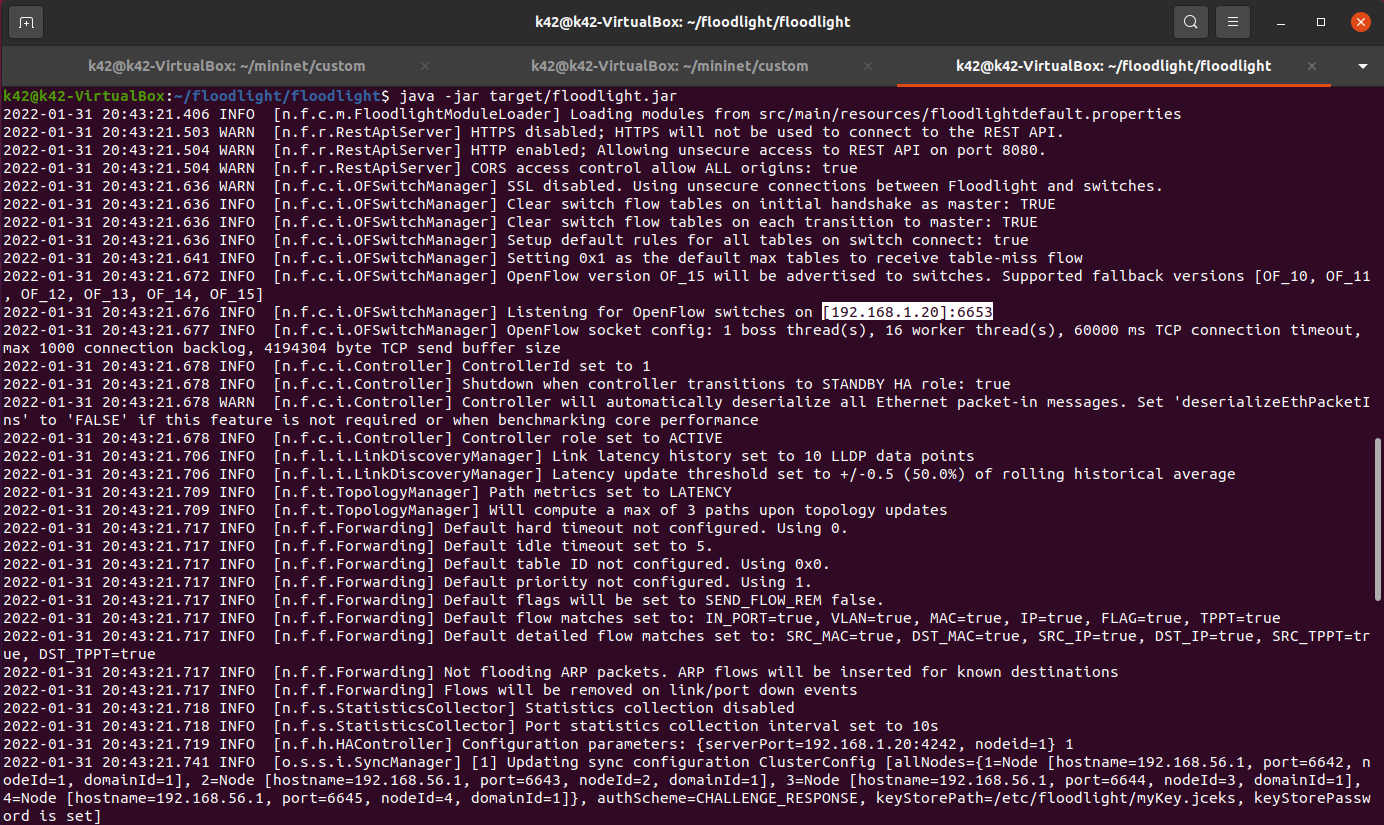
\includegraphics[width=1.0\textwidth]{Bilder/floodlight}
 \captionsetup{justification=centering,margin=1cm}
 \caption{Ausführung von Floodlight über den Linux-Terminal}
 \label{floodlight}
\end{figure}

\subsection{Ergebnis}
{\tiny Verfasst von: Tung\par}
\begin{wrapfigure}{r}{0.5\textwidth}
	\vspace{-\baselineskip}
    \centering
    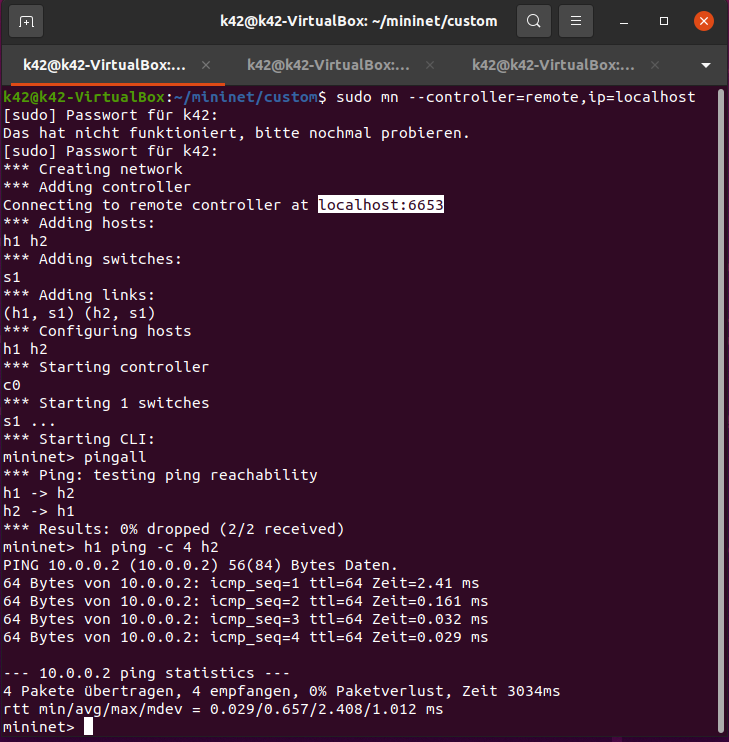
\includegraphics[width=0.5\textwidth]{Bilder/ping}
    \caption{Mininet Controller Verbindung und Ping-Test}
    \label{ping}
\end{wrapfigure}

Nach der Ausführung von Floodlight, wurde dieser mit einer OpenFlow-fähigen Switch verbunden. Der Switch wurde mit Mininet mit der Angabe des Controllers simuliert. Die Konsole zeigt die erfolgreiche Verbindung mit dem Controller. Die Konnektivität im Netzwerk kann mit dem Befehl \textit{\textbf{pingall}} überprüft werden. Die Konnektivität zwischen Host 1 und Host 2 wird durch den Befehl \textit{\textbf{h1 ping h2}} getestet. Durch Wireshark kann der ausgelöste Datenverkehr betrachtet werden (siehe Abbildung \ref{ping}).



\chapter{Durchführung des Projektes}
{\tiny Verfasst von: James\par}
Die in Kapitel 1.3 dargestellten Problemstellungen werden in diesem Kapitel behandelt und realisiert. Mit den im vorherigen Kapitel erläuterten Werkzeugen wird dieses Projekt umgesetzt. Durch Abbildungen, Code Ausschnitte und Erläuterungen soll die Dokumentation die Vorgehensweise und Überlegungen der Gruppe wiedergeben. 



\section{Netzwerkplan}
{\tiny Verfasst von: Tung, Naghmeh, James, Mücahit\par}
Die topologische Struktur des Netzwerks, die in Mininet erstellt wird, ist in Abbildung \ref{netzwerkplan} dargestellt. Das Netzwerkdiagramm enthält 40 Hosts, 4 Switches, 4 Router und einen Controller. Der Floodlight-Controller hat einen globalen Überblick über die physikalische Topologie. Die 4 Switches sind mit dem Controller verbunden. Zehn Hosts in den jeweiligen Lokationen sind mit einem Switch verbunden. Um die Hosts in jeder Lokation mit dem Internet und mit anderen Lokationen zu verbinden, wird ein Router benötigt. Durch die grüne Linie und den Tunnel wird gezeigt, dass die Kommunikation zwischen Lokationen verschlüsselt sind. Ebenfalls sind alle Router der Lokationen mit dem Internet verbunden, welches durch eine Cloud visualisiert wird.

\begin{figure}[H]
 \centering
 \makebox[\textwidth][c]{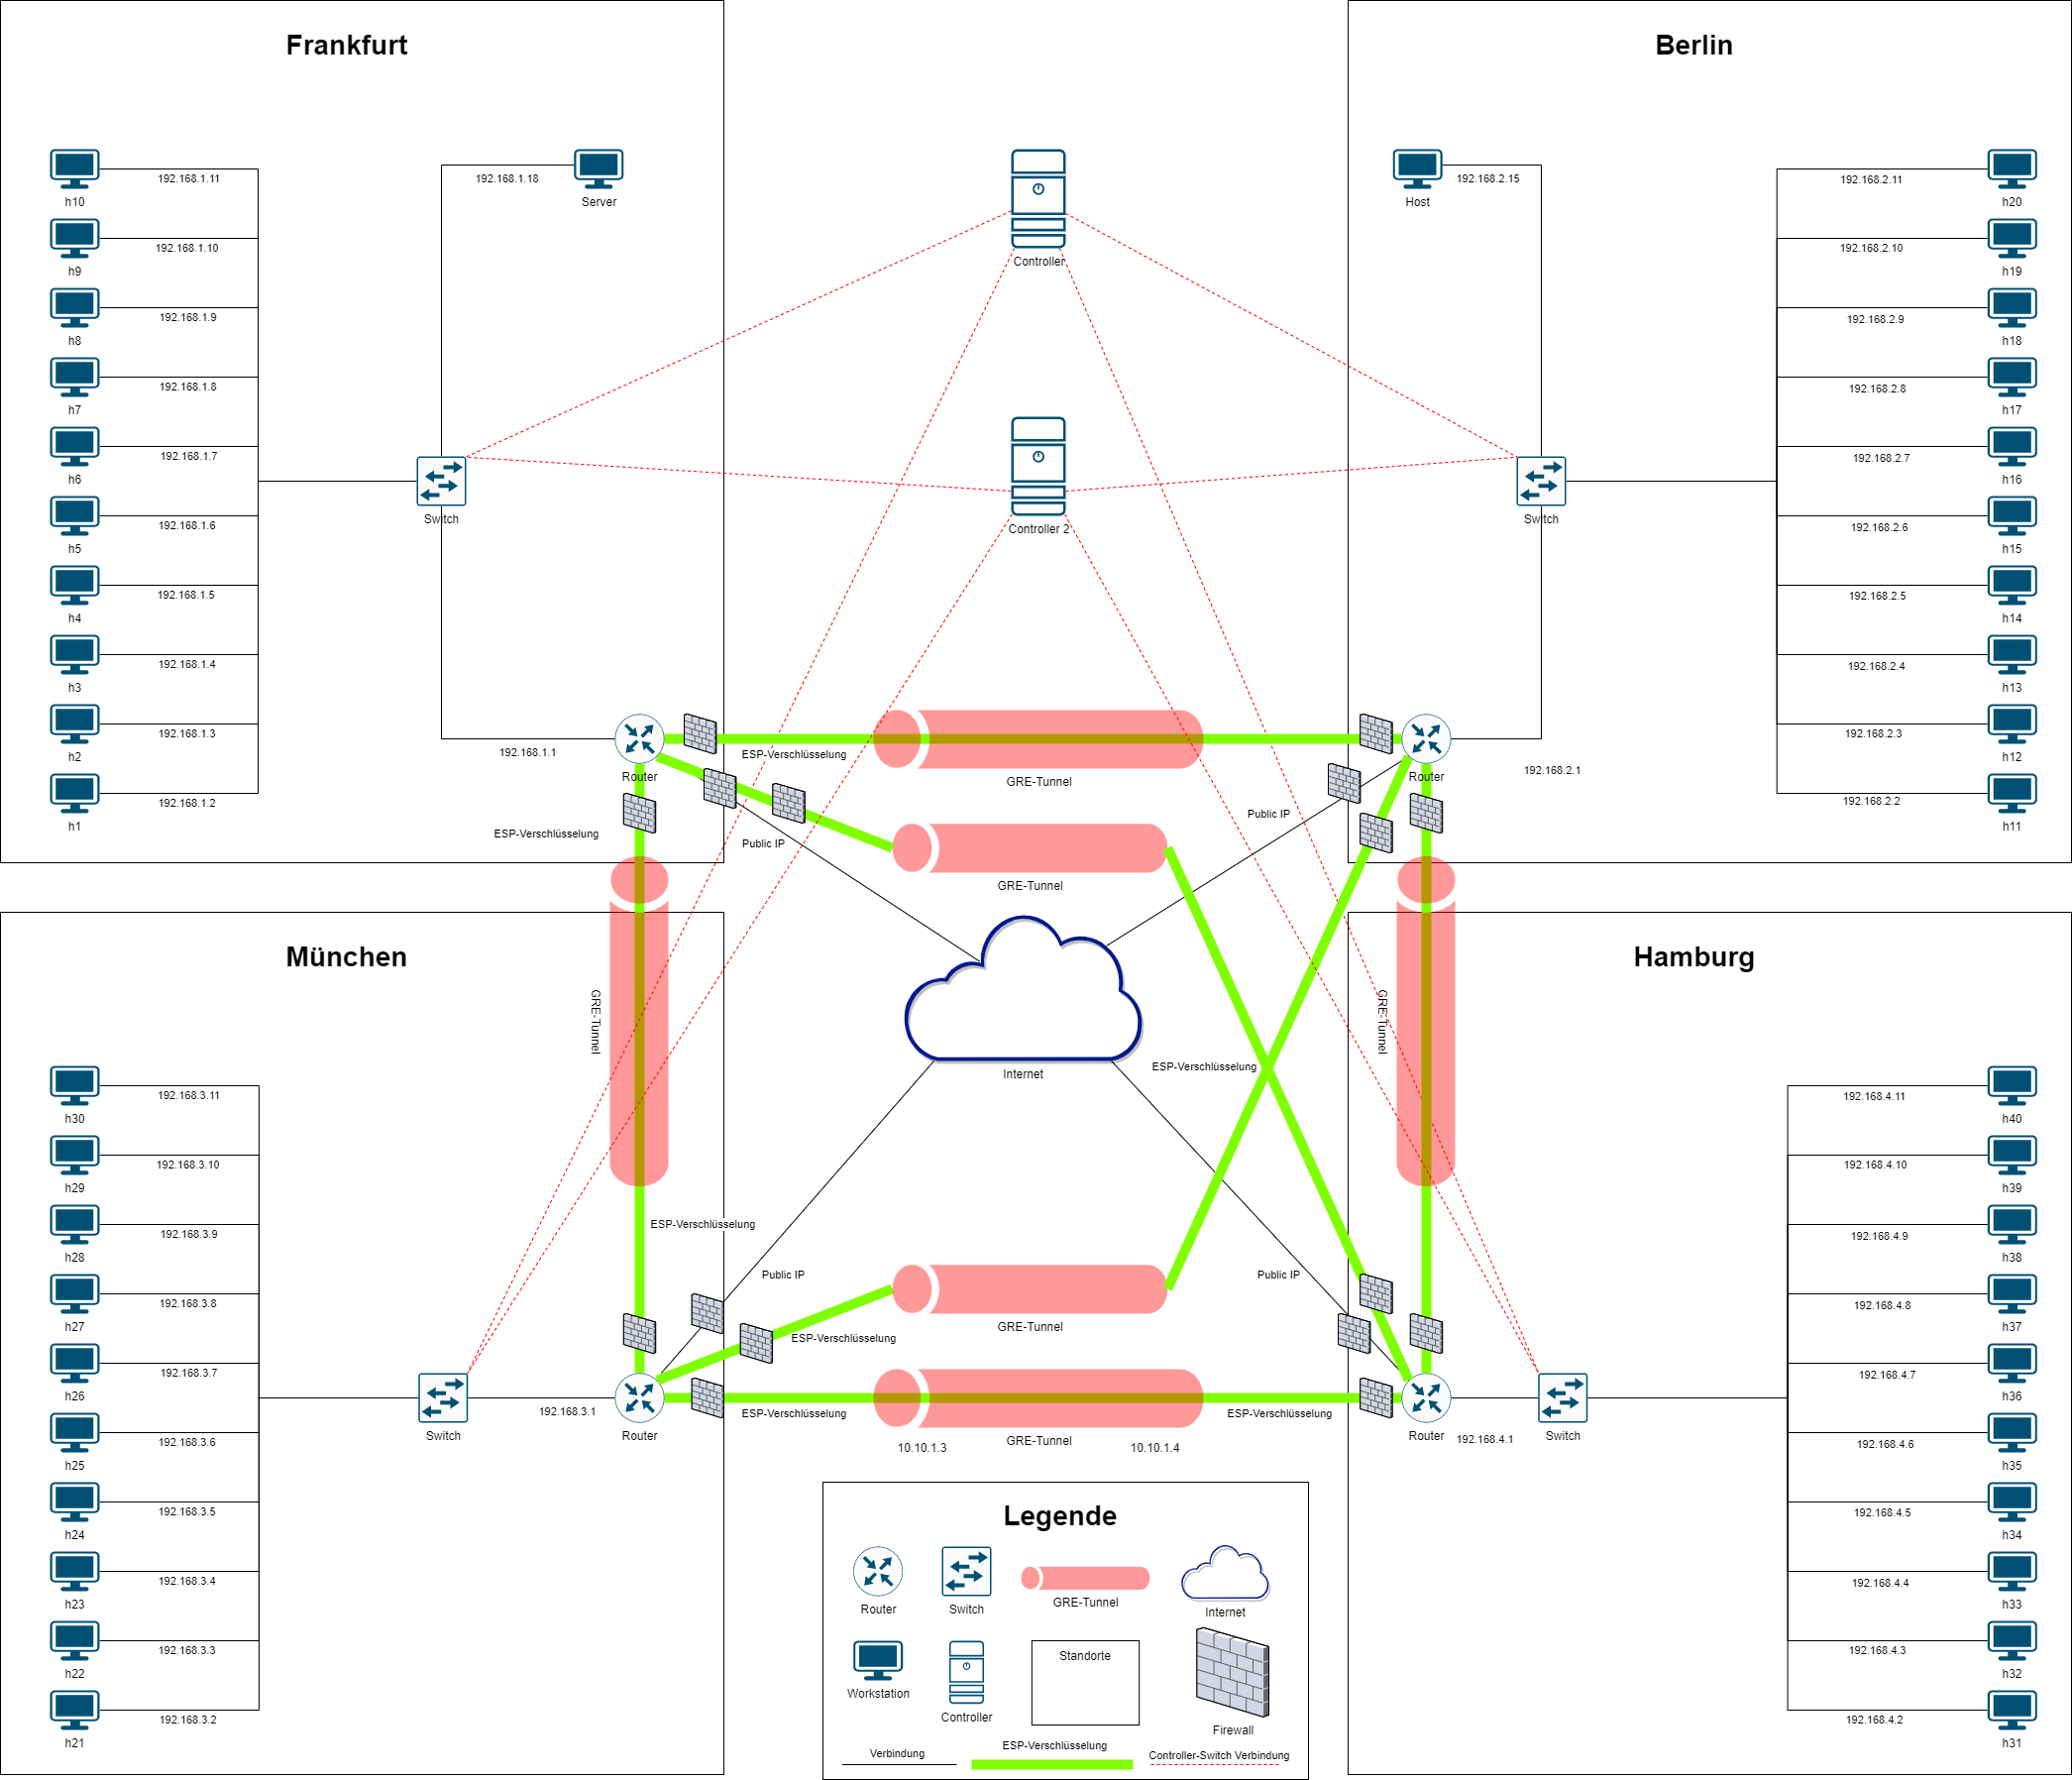
\includegraphics[width=1.1\textwidth]{Bilder/netzwerkplan}}
 \captionsetup{justification=centering,margin=1cm}
 \caption{Netzwerkplan aller Lokationen}
 \label{netzwerkplan}
\end{figure}

\begin{table}[H]
	\caption{Vergabe von IPv4-Adressen im Netzwerk}
	\label{netzwerkplan-addressen}
	\centering
	\hspace*{-1cm}
	\begin{tabular}{p{3.5cm} p{3cm} p{3cm} p{3cm} p{3cm}}
		\toprule
		 Standort & Frankfurt & Berlin  & München & Hamburg \\
		\midrule 
		Subnetz & 192.168.1.0/24 &  192.168.2.0/24 & 192.168.3.0/24 & 192.168.4.0/24\\
		
		Netzwerkmaske	&255.255.255.0& 255.255.255.0& 255.255.255.0	& 255.255.255.0 \\
		
		Broadcast & 192.168.1.255 &	192.168.2.255 &	192.168.3.255 & 192.168.4.255\\
		
		Router & 192.168.1.1&192.168.2.1& 192.168.3.1 &192.168.4.1\\
		
		Switch & 192.168.1.20& 192.168.2.20&192.168.3.20&	192.168.4.20\\
		
		erster Host& 192.168.1.2& 192.168.2.2& 192.168.3.2&192.168.4.2\\
		
		letzter Host& 192.168.1.254 & 192.168.2.254 & 192.168.3.254 & 192.168.4.254\\
		
	\end{tabular}
	
\end{table}

\section{Aufbau des Netzwerkgerüstes in Mininet}
In diesem Abschnitt wird die beschriebene Topologie unter Verwendung von Mininet simuliert und erklärt.

\subsection{Durchführung}
{\tiny Verfasst von: Tung\par}
In der Main-Funktion werden die Komponenten eines Netzwerks deklariert und aufgerufen. Das sind eine Topologie, ein Controller mit zugewiesenem Port und ein Mininet Objekt mit der deklarierten Topologie. Anschließend wurde für unsere Router Routing-Regeln und Informationen gegeben.

\subsection{Aufbau der Topologie}
{\tiny Verfasst von: Tung, Mücahit\par}
Die Klasse Netzwerk bildet die Netzwerktopologie. Diese befindet sich in der Main-Funktion des Mininet-Skripts. Das Mininet-Skript besteht aus einer Main-Funktion. Die Main-Funktion enthält eine definierte Klasse \textit{\textbf{Netzwerk()}}. Mithilfe dieser Klasse wird das Netzwerk beziehungsweise eine Topologie erstellt (siehe Abbildung \ref{mininet1}). Die Klasse übernimmt ein Topo-Objekt an dem er mit der in ihm definierten \textit{\textbf{build()}} Methode die Konfiguration des Netzwerkes vornimmt. In der \textit{\textbf{build()}} Methode wird zuerst ein String definiert, der den privaten-IP-Bereich der vier Lokationen enthält. Der \textit{\textbf{defaultIP}} String bleibt in unvollständiger Form \textit{\textbf{192.168.\%s.1/24}}. Somit kann er später durch passende Stellen ersetzt und genutzt werden. Lediglich ist hier im dritten Block ein Platzhalter eingesetzt der beim Erstellen der Router in einer Schleife durch die Zahl der Iteration ersetzt wird. Zunächst wird ein leeres Array/Liste unter dem Namen Routers deklariert. Dies wird dann später genutzt und mit den Router-Objekten gefüllt. Später für die Verlinkung der Router mit dem jeweiligen Switch wird die Liste aufgerufen. Für größere Anzahl von Router ist die Bedeutung der Liste sehr praktisch.

\begin{figure}[H]
 \centering
 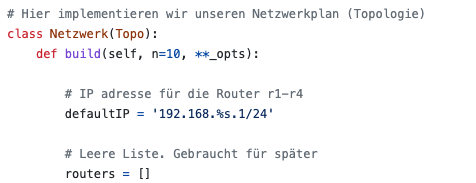
\includegraphics[width=0.6\textwidth]{Bilder/mininet1}
 \captionsetup{justification=centering,margin=1cm}
 \caption{Netzwerk-Klasse zur Topologie Erstellung}
 \label{mininet1}
\end{figure}

Im nächsten Teil der Klasse Netzwerk, werden die Komponenten des Netzwerks implementieren. Dies ist mit Hilfe einer Schleife mit 4 Durchläufen ausgeführt worden. Jeder Durchlauf entspricht einer Lokation, der jeweils einen Switch, einen Router und zehn Hosts erstellt. Dabei wird bei jeder Iteration erst ein Router-Objekt mit der Methode \textit{\textbf{self.addNode()}} erstellt, bei dem der Name, der private IP-Adressen-Bereich, die MAC-Adresse und der benutzerdefinierte Parameter für die Konfiguration, dass der Router IP-Forwarding aktiviert bekommt, übergeben. Danach wird der Router der vorher erstellten Liste eingefügt. Mit der Methode \textit{\textbf{self.addSwitch()}} wird ein Switch erstellt der einen Namen erhält. Anschließend wird mit der Methode \textit{\textbf{self.addLink()}} eine Verbindung zwischen dem Router und der Switch erstellt. Dabei wird auch die Netzwerkschnittstelle des Routers benannt und der private-IP-Adressenbereich vergeben  (siehe Abbildung \ref{mininet2}).

\begin{figure}[H]
 \centering
 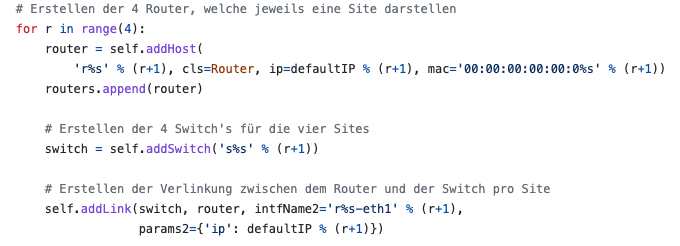
\includegraphics[width=0.7\textwidth]{Bilder/mininet2}
 \captionsetup{justification=centering,margin=1cm}
 \caption{Erstellung und Verbindung von Router und Switch}
 \label{mininet2}
\end{figure}

Danach folgt noch eine Schleife, bei der insgesamt n Hosts erstellt und mit dem Switch verbunden werden (siehe Abbildung \ref{mininet3}). Die Hosts erhalten für den jeweiligen privaten-IP-Bereich eine IP, eine MAC-Adresse und die IP des jeweiligen Routers als Standard-Route zugewiesen.
 
\begin{figure}[H]
 \centering
 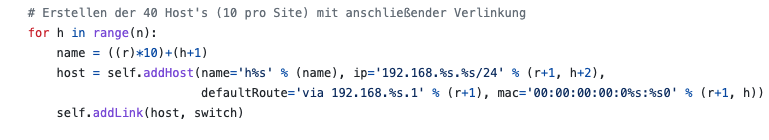
\includegraphics[width=0.8\textwidth]{Bilder/mininet3}
 \captionsetup{justification=centering,margin=1cm}
 \caption{Erstellung und Verbindung von Hosts und Switch}
 \label{mininet3}
\end{figure}

Nachdem für alle Lokationen der Rumpf erstellt worden ist, werden die Verbindungen zwischen den Routern mit dem Befehl \textit{\textbf{self.addLink()}} hergestellt. Dabei wird jeder Router mit allen anderen Routern verbunden. Dieser Vorgang wird das Internet simulieren, worauf ebenfalls der Tunnel und die Verschlüsselung implementiert wird. Dabei wird der Netzwerkschnittstellen-Name für beide Router und die jeweilige öffentliche-IP-Adresse definiert. Zusätzlich wird per \textit{\textbf{bw=20}} Befehl die Bandbreite der Leitung auf 20 Megabit gesetzt, wobei dies die geforderte SDSL-Leitung im Kapitel 3.8 darstellen soll (siehe Abbildung \ref{mininet4}).

\begin{figure}[H]
 \centering
 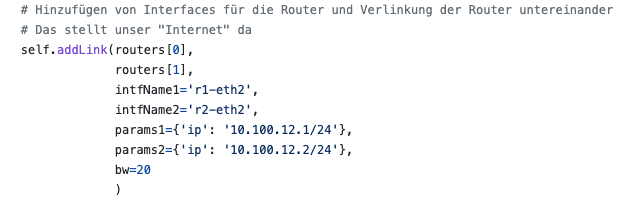
\includegraphics[width=0.7\textwidth]{Bilder/mininet4}
 \captionsetup{justification=centering,margin=1cm}
 \caption{Verbindung und Konfigurierung der Router}
 \label{mininet4}
\end{figure}



\subsection{Controller Implementierung}
{\tiny Verfasst von: Tung, Mücahit\par}
Nach der Erstellung der Topologie geht es weiter bei der Main-Funktion. Es wird ein \textit{\textbf{RemoteController-Objekt}} erstellt, der einen Namen, die Konfiguration, um was für ein Controller es sich handelt, die IP-Adresse und den Port, wo er zu erreichen ist, bekommt (siehe Abbildung \ref{mininet5}). Hier ist wichtig zu erwähnen, dass der Controller auf Ubuntu läuft und zurzeit per \textit{\textbf{localhost}} zu erreichen ist. Der Controller könnte auf einer anderen VirtualBox-Maschine laufen und per \textit{\textbf{internes Netzwerk}} verbunden werden. Ebenfalls kann der Controller auf dem Hostsystem laufen und per \textit{\textbf{Host-Only-Adapter}} in Mininet eingebunden werden \cite{mnvm}. 

\begin{figure}[H]
 \centering
 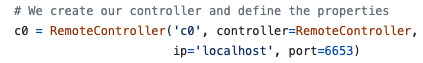
\includegraphics[width=0.7\textwidth]{Bilder/mininet5}
 \captionsetup{justification=centering,margin=1cm}
 \caption{Erstellung eines RemoteController's}
 \label{mininet5}
\end{figure}

Anschließend wird ein Mininet-Objekt erstellt, bei dem die erstellte Topologie, der erstellte Controller, ein \textit{\textbf{TCLink-Objekt}} für die Einstellung der Bandbreite der Netzwerkadapter und ein \textit{\textbf{OVSKernelSwitch-Objekt}} für die Erstellung der Switches als \textit{\textbf{Open vSwitches}} (siehe Abbildung \ref{mininet6}). Diese werden später verwendet, um den Quality of Service zu implementieren. Dabei werden per \textit{\textbf{ovs-vsctl-Befehle}} Queues an den Ports der Switches erstellt und die Priorisierung der Pakete vorgenommen \cite{qosovs}.

\begin{figure}[H]
 \centering
 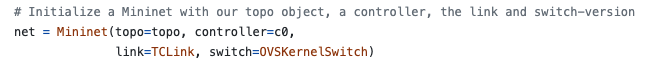
\includegraphics[width=1.0\textwidth]{Bilder/mininet6}
 \captionsetup{justification=centering,margin=1cm}
 \caption{Erstellung des Mininet-Objektes}
 \label{mininet6}
\end{figure}

\subsection{Ergebnis}
{\tiny Verfasst von: Tung\par}
Wenn das Mininet Skript ausgeführt wird, ist eine Topologie mit 40 Hosts über 4 Switches und 4 Routers zu sehen. Durch \textit{\textbf{pingall}} kann es festgestellt werden, dass alles richtig funktioniert hat (siehe Abbildung \ref{pingall}).

\begin{figure}[H]
 \centering
 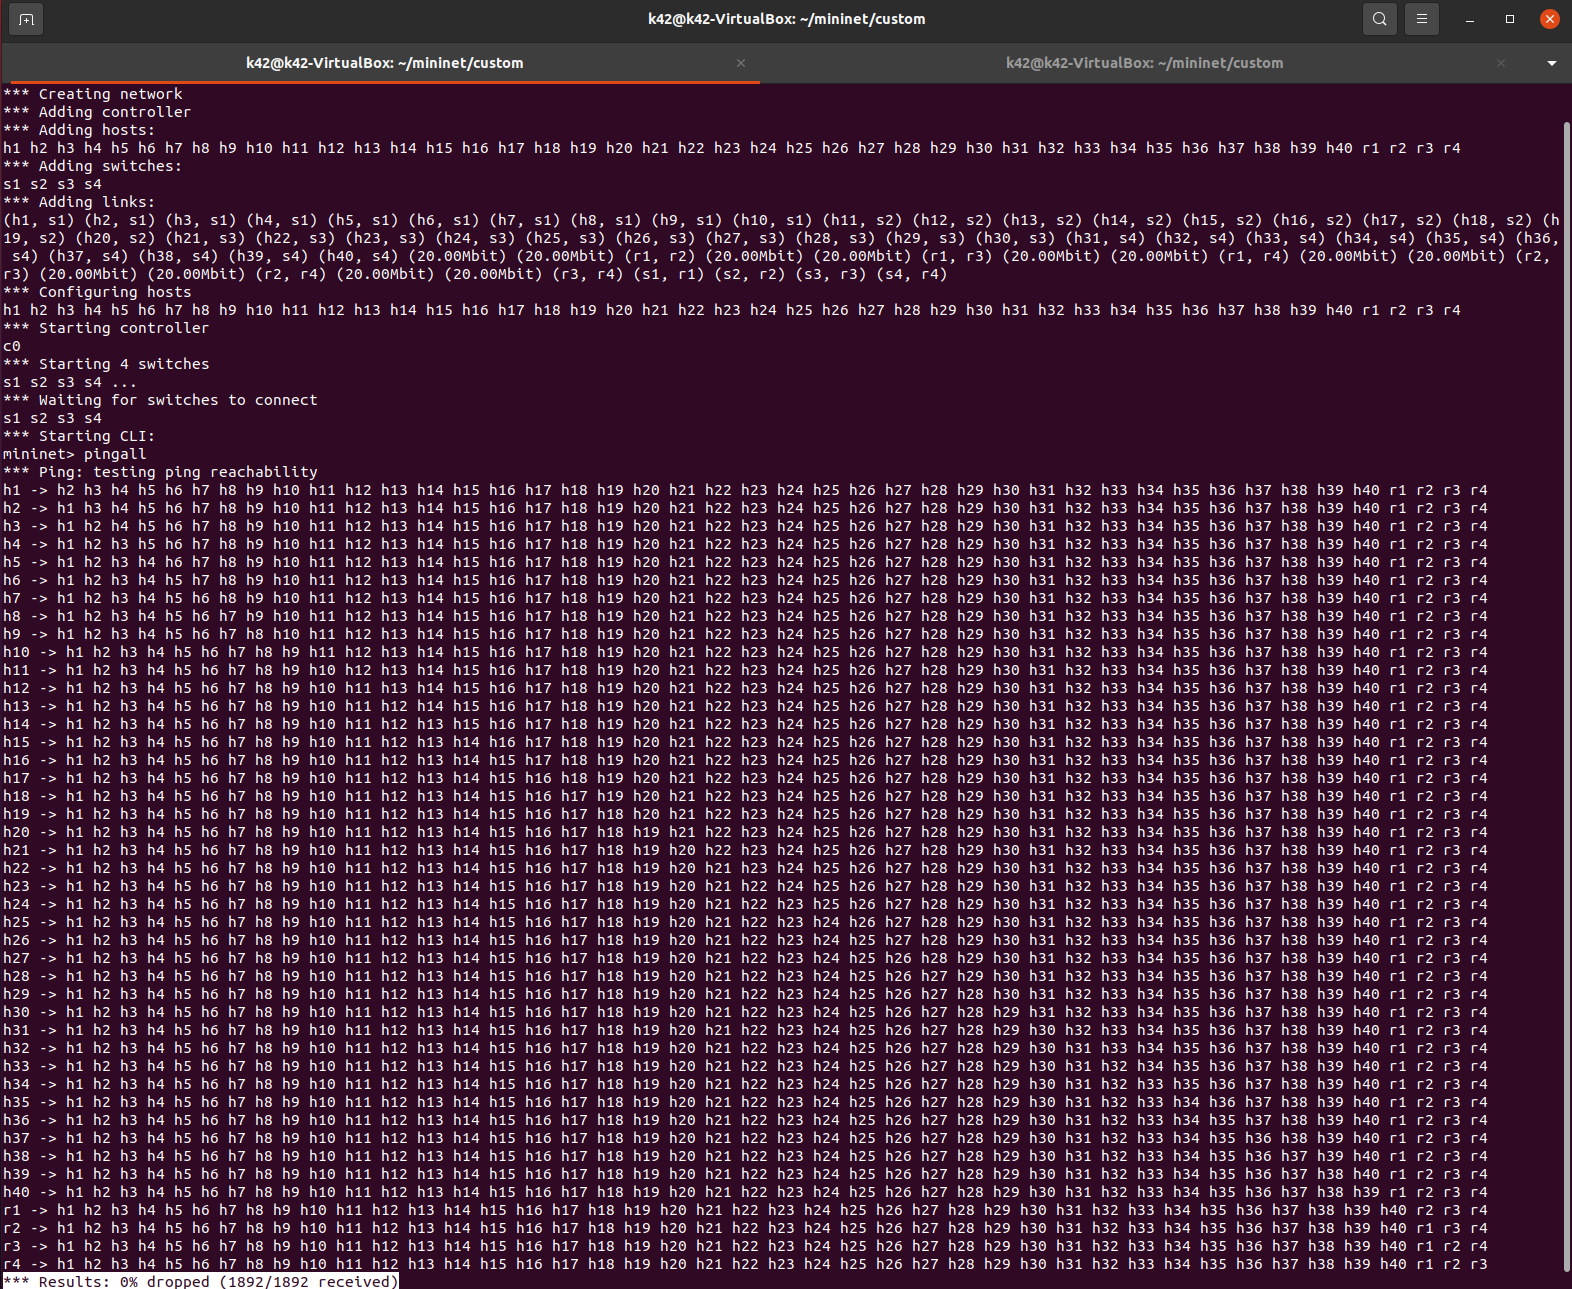
\includegraphics[width=1.0\textwidth]{Bilder/pingall}
 \captionsetup{justification=centering,margin=1cm}
 \caption{Ausführung und Testen vom Mininet-Skript}
 \label{pingall}
\end{figure}

\newpage
\section{Verschlüsselung der Netzwerkverbindung zwischen den Lokationen}
{\tiny Verfasst von: Mücahit\par}
Zwischen den vier Lokationen soll ein Tunnel über das Internet konfiguriert werden. Dieser wird auch Virtual Private Network (VPN) genannt. Der gesamte Datenverkehr durch den Tunnel soll verschlüsselt und für unbeteiligte nicht einsehbar sein.

\subsection{Vorüberlegung}
{\tiny Verfasst von: Mücahit\par}
Der Tunnel wird zwischen den Routern r1-r4 entstehen und für eine Verbindung der Netzwerke der Lokationen sorgen. Damit soll eine \textit{\textbf{Site-to-Site-VPN}} Verbindung zwischen allen Lokationen hergestellt werden \cite{sitetosite}. Dieser zeichnet sich durch die Verschlüsselung ab den Schnittstellen, also den Routern der Lokationen, aus. Zudem werden aus dem privaten Netzwerk eingehende Pakete an den Routern verschlüsselt und weiterverschickt. Der Router an der Ziellokation wird das Paket entschlüsseln und an die Zieladresse weiterleiten. Die Methode, die implementiert werden soll, heißt \textit{\textbf{IPSEC over GRE}} und soll alle angestellten Vorüberlegungen ermöglichen \cite{vpntunnel}.

\subsection{Durchführung}
{\tiny Verfasst von: Mücahit\par}
Für die Durchführung folgt in der Main-Funktion des Mininet-Skripts die Einrichtung der Tunnel zwischen den Routern beziehungsweise den Lokationen. Dafür baut jeder Router mit jedem Router einen GRE-Tunnel auf, für den der Befehl \textit{\textbf{ip tunnel add Tunnel-Name mode gre local Schnittstelle\hyp{}Router\hyp{}Lokation\hyp{}A remote Schnittstelle\hyp{}Router\hyp{}Lokation\hyp{}B ttl 255}} bei jedem Router über die Mininet-Methode \textit{\textbf{info(net[‘Router\hyp{}Name'].cmd(Befehl))}} ausgeben und ausgeführt wird (siehe Abbildung \ref{gre}). Nachdem die Verbindung definiert wurde, wird der Tunnel-Adapter per \textit{\textbf{ip link set Tunnel-Name up}} hochgefahren. Anschließend wird dem Tunnel Adapter mit dem Befehl \textit{\textbf{ip addr add Tunnel-IP dev Tunnel-Name}} die Tunnel IP vergeben. Hier ist wichtig, dass der IP-Adressbereich zwischen zwei Lokationen im selben Bereich liegt. Hier erfolgt das gleiche Prinzip wie bei der Erstellung und Simulierung des Internets zwischen den Lokationen \cite{tunnelimpl}.

\begin{figure}[H]
 \centering
 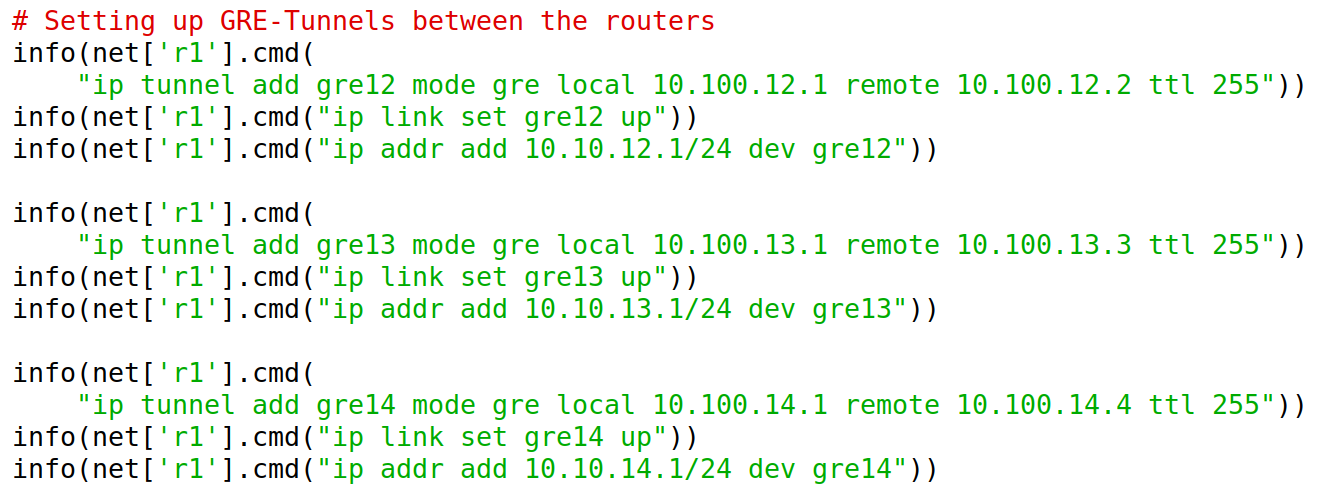
\includegraphics[width=0.75\textwidth]{Bilder/gre}
 \captionsetup{justification=centering,margin=2cm}
 \caption{Aufstellen der GRE-Tunnel}
 \label{gre}
\end{figure}

Nachdem der Tunnel aufgesetzt worden ist, sind alle Pakete, die durch den Tunnel versendet werden, nun als Payload eines neuen Paketes, wo der neue IP-Header der IP des Tunnels entspricht \cite{newpayload} (siehe Abbildung \ref{ipsecgre}). Daraus folgt, dass nun Pakete, die die Maximum Transmission Unit (MTU) erreichen, jetzt eine geringere Länge annehmen müssen, da der neue Payload aus dem ursprünglichen Payload und IP-Header besteht. Wenn der Fall eintritt, schickt der Router eine Aufforderung an den Absender zurück, das Paket kleiner zu gestalten \cite{MTU}.

\begin{figure}[H]
	\centering
	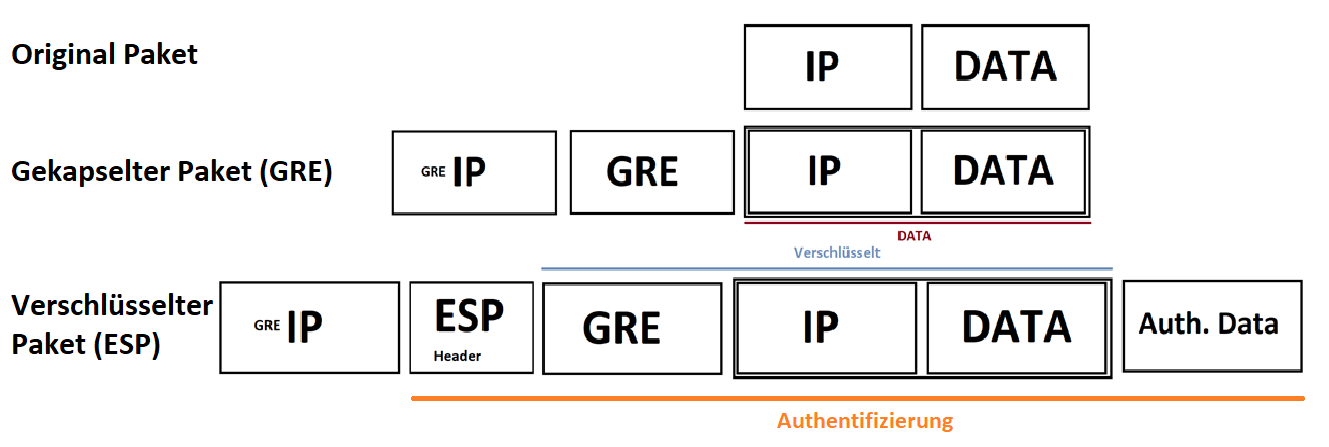
\includegraphics[width=0.8\textwidth]{Bilder/ipsecgre}
	\captionsetup{justification=centering,margin=2cm}
	\caption{Wandlung der Pakete bei IPSEC over GRE}
	\label{ipsecgre}
\end{figure}

Im nächsten Schritt wird die Route zum jeweils anderen Subnetzwerkadressenbereich per \textit{\textbf{ip route add IP-anderen-Lokation via IP-Adapter dev Adapter-Name}} Befehl in die Routing-Tabelle eingefügt \cite{addroute} (siehe Abbildung \ref{route}). Da es sich hierbei um eine Simulation handelt, sollten alle Lokationen einen jeweils anderen privaten Adressenbereich besitzen. Bei Überschneidungen könnte es zu Problemen führen. Bei einer echten Umgebung mit echten öffentlichen IP-Adressen könnten dieselben privaten IP-Adressen für verschiedene Lokationen genutzt werden. Dies wird in der Realität üblicherweise so gemacht.

\begin{figure}[H]
 \centering
 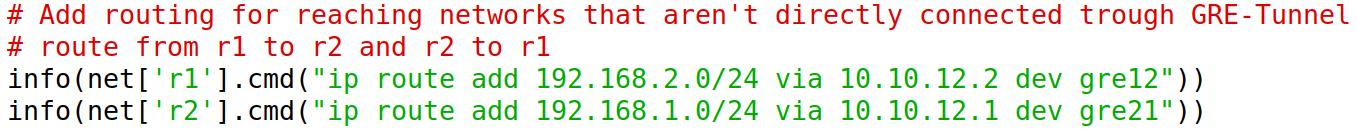
\includegraphics[width=1.0\textwidth]{Bilder/route}
 \captionsetup{justification=centering,margin=2cm}
 \caption{Konfiguration der Routen}
 \label{route}
\end{figure}


Der Tunnel von und zu den Lokationen ist nun aufgesetzt. Als Nächstes sollen alle Pakete aus dem privaten IP-Adressenbereich bei der Übermittlung durch den Router verschlüsselt und weitergeleitet werden. Dazu sollen alle Pakete von außen entschlüsselt und zum Zielort weitergeleitet werden. Für diese Methode wird die Verschlüsselung und Entschlüsselung über IPSEC im Transport-Modus mit dem Encapsulating Security Payload (ESP) Protokoll benutzt. Dafür wird zuerst der Befehl \textit{\textbf{ip xfrm state add src IP-Adresse-des-Routers dst IP-Adresse-des-Ziel-Routers proto esp Security-Parameter-Index-Key enc ‘cbc(aes)‘ 256bit-Key mode transport}} ausgeführt, um Regeln für die Ver- und Entschlüsselung auf dem Router einzufügen \cite{esp}. Jeder Router bekommt zwei Regeln für jeweils einen anderen Router. Eine Regel ist für die Entschlüsselung bei ankommenden Paketen und die andere Regel für die Verschlüsselung bei abgehenden Paketen (siehe Abbildung \ref{state}).

\begin{figure}[H]
 \centering
 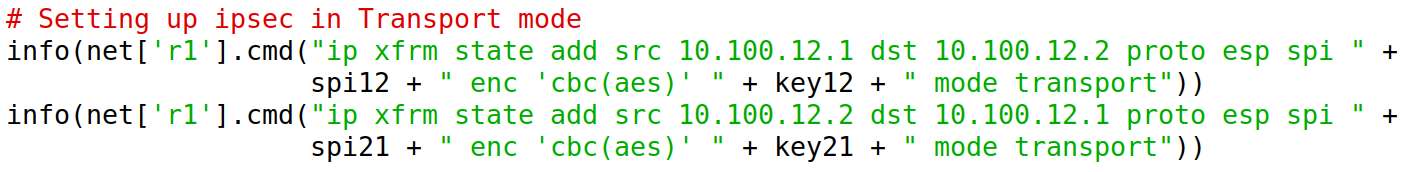
\includegraphics[width=1.0\textwidth]{Bilder/state}
 \captionsetup{justification=centering,margin=2cm}
 \caption{Erstellung der States für die Ver- und Entschlüsselung}
 \label{state}
\end{figure}

Der Befehl legt für Pakete mit bestimmter IP-Quelladresse, IP-Zieladresse, einem Security-Parameter-Index Key (SPI) und einer 256 Bit Verschlüsselung fest, bei einer Übereinstimmung das Paket zu verschlüsseln oder zu entschlüsseln. Auf Abbildung \ref{ipsecgre} kann der Wandel von der ursprünglichen Paketstruktur auf die verschlüsselte Paketstruktur nachvollzogen werden. Es wird für eingehende und ausgehende Pakete jeweils eine Regel festgelegt. Der Unterschied ist, dass die IP-Ziel- und Quelladresse, der Security-Parameter-Index-Key und die 256 Bit Verschlüsselung verschieden sind. Durch die States wurden die Ver- und Entschlüsselungen auf den Routern installiert. Die Keys und SPI’s wurden zufällig gewählt. Nun muss den Routern angewiesen werden, auf welchem Datenverkehr die installierten States angewandt werden sollen. Dies geschieht über Policies. Dort wird über den \textit{\textbf{ip xfrm policy add dir out src IP-Adresse-des-Routers dst IP-Adresse-des-Ziel-Routers tmpl proto esp mode transport}} Befehl die Anweisung erteilt, dass auf den IP-Ziel- und Quelladressen die Ver- und Entschlüsselung stattfinden soll. Dabei muss der Befehl zweimal eingegeben werden, wobei die IP-Adressen vertauscht werden (siehe Abbildung \ref{policy}). Es wird nicht die Tunnel-IP, sondern die Router-IP angegeben \cite{xfrm}.

\begin{figure}[H]
 \centering
 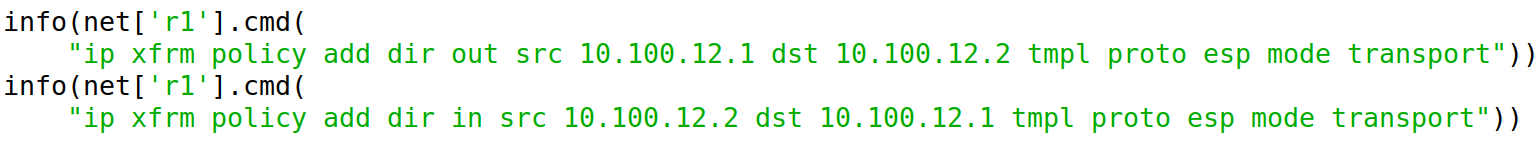
\includegraphics[width=1.0\textwidth]{Bilder/policy}
 \captionsetup{justification=centering}
 \caption{Erstellung der Policies für die Ver- und Entschlüsselung}
 \label{policy}
\end{figure}

\subsection{Ergebnis}
{\tiny Verfasst von: Mücahit\par}
Durch die Erstellung der Tunnel und der Verschlüsselung der Pakete wurde die komplette Kommunikation zwischen den Lokationen sicherer. Dazu gehört unter anderem die Authentifizierung des Kommunikationspartners und der Verhinderung unautorisierter Veränderungen von Paketen \cite{espsecurity}. Zwischen den Lokationen war vorher der gesamte Datenverkehr ersichtlich, wohingegen jetzt alles verschlüsselt ist (siehe Abbildung \ref{esp}).

\begin{figure}[H]
 \centering
 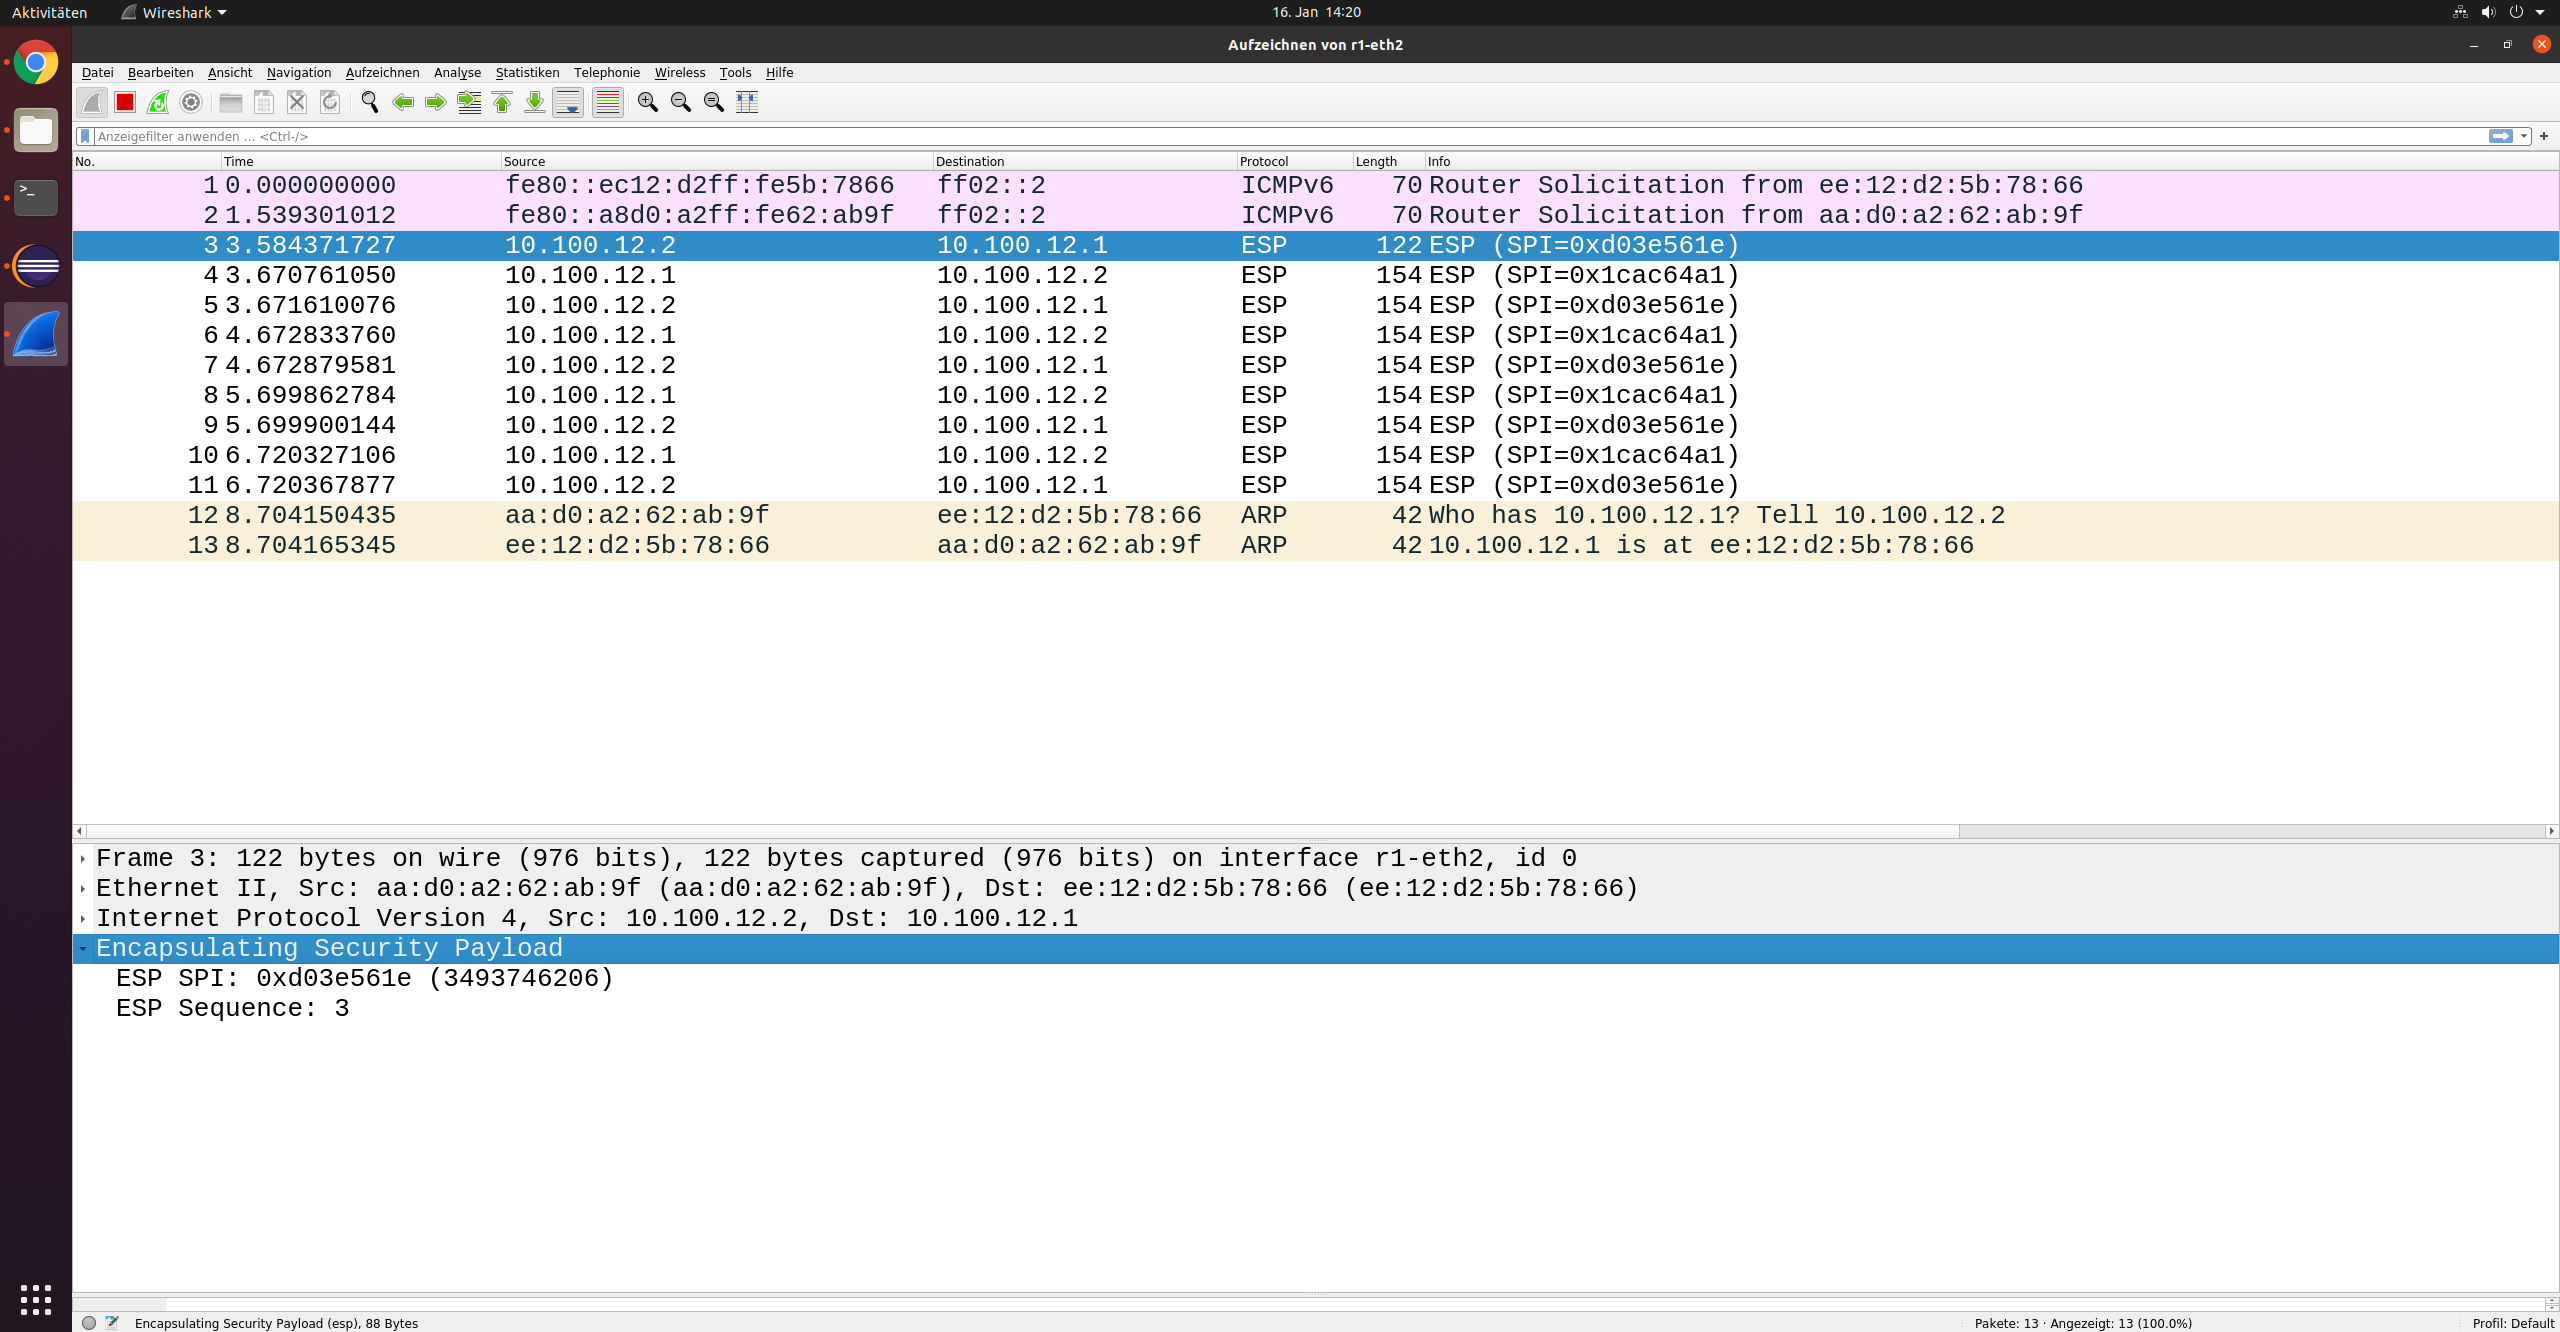
\includegraphics[width=1.0\textwidth]{Bilder/esp}
 \captionsetup{justification=centering}
 \caption{Verschlüsselter Verkehr zwischen Standort Frankfurt und Berlin}
 \label{esp}
\end{figure}


\section{Auswahl des Service-Providers}
{\tiny Verfasst von: Tung, Naghmeh, James, Mücahit\par}
Alle Lokationen sind über einen Tunnel durch das Internet miteinander verbunden. Deswegen benötigen alle Lokationen eine DSL-Verbindung mit der richtigen Konfiguration zur Realisierung. Der Preis und die Bandbreite der DSL-Leitung zählen bei der Auswahl als primäre Faktoren. Zusätzlich können weitere Leistungen betrachtet werden.\par 
Im Folgenden sind in einer Tabelle die Internet-Service-Provider O2, Vodafone, 1\&1 und Telekom mit verschiedenen Bandbreiten und den dazugehörigen Nettopreisen aufgelistet \cite{o2} \cite{vodafone} \cite{1u1} \cite{telekom} (siehe Tabelle \ref{dsl}). Die Angebote sind aktuell und aus den originalen Webseiten der Provider entnommen worden.

\begin{table}[H]
\caption{DSL-Angebote verschiedener Internet-Service-Provider}
\label{dsl}
\centering
  \begin{tabular}{p{1.5cm} p{2.5cm} p{4cm} p{4cm} p{2.4cm}} 
\toprule
    Anbieter & Tarife & Download in Mbit/s (min/normal/max) & Upload in Mbit/s (min/normal/max)& Monatl. Preis (Netto, 24 Monate) \\
\midrule 
    	Telekom & Company Start 16 &  6,3 / 9,5 / 16 & 0,7 / 1,5 / 2,4 & 37 Euro\\
    	&Company Start 50&27,9 / 47 / 50&2,7 / 9,4 / 10& 42 Euro\\
	&Company Start 100&54 / 83,8 / 100&20 / 33,4 / 40& 47 Euro\\
	&Company Start 250&175/ 200 / 250&20 / 35 / 40& 57 Euro\\
	&Company Start 500&400 / 500/ 500&80/ 100/ 100& 70 Euro\\
	&Company Start 1000&700/ 850 / 1000&200 / 200 / 200& 100 Euro\\
	1\&1	&DSL 16	&6,6 / 11 / 16	&0,128 / 0,983 / 1		& 20 Euro\\
 	&DSL 50	&16,7/ 44 / 50&	1,6 / 9,6 / 10&		22,5 Euro\\
 	&DSL 100	&54 / 88,6 / 100	&20 / 36,9 / 40&		25 Euro\\
 	&DSL 250&	175/ 200/ 250	& 20 / 35 / 40		& 30 Euro\\
	&Glasfaser 500&	431/ 250/ 480	 &215/ 225/ 240	&	200 Euro\\
 	&Glasfaser 1.000&	860/ 900/ 1000	&430/ 450/ 500&	350 Euro\\
	Vodafone& Plus 16 Regio DSL&	6 / 9,5 / 16&	0,7 / 0,9 / 1&		20 Euro\\
 	&Plus 50 Regio DSL&	28 / 38 / 50&	2,7 / 7,5 / 10&		22,5 Euro\\
 	&Plus 100 Regio DSL&	54 / 87/ 100&	20 / 37 / 40&		25 Euro\\
 	&Plus 250 Regio DSL&	175/ 210/ 250& 	20/ 37/ 40	&	30 Euro\\

	
	O2 &MyOffice S&	0,3/ 8 / 10	& 0,3 / 1,5 / 2&		25 Euro\\
 	&MyOffice M&	3/ 38 / 50&	0,7 / 8 / 10&		27,5 Euro\\
 	&MyOffice L&	50/ 83/ 100&	10 / 33/ 40&		30 Euro\\
 	&MyOffice XL&	105/ 200 / 250&	12/ 33 / 40&		35 Euro\\

  \end{tabular}

\end{table}

\newpage
Die notwendige Bandbreite für den Download und Upload wurde in der Gruppe abgestimmt. Vorher wurden kleine Tests zur Belegung und Stärkung der Argumente für die Abstimmung gemacht. Bei der Abstimmung wurde pro Arbeitsplatz mindestens 10 Megabit als Download und 5 Megabit als Upload für einen flüssigen Arbeitsrhythmus als notwendig gesehen. Demnach sind bei zehn Arbeitsplätzen ein Upload von mindestens 50 Megabit und ein Download von mindestens 100 Megabit nötig. Nach dem Preisleistungsverhältnis ist der Telekom Company Start 500 \cite{companystart} Angebot mit einer garantierten Uploadrate von mindestens 80 Megabit und einer garantierten Downloadrate von mindestens 400 Megabit die beste Wahl. Zusätzlich besitzt die Telekom jahrelange Erfahrung und beweist dadurch gute Qualitäten, welches die Entscheidung für das Produkt noch einmal gestärkt hat.\par
Neben einer DSL-Leitung benötigen die Lokationen eine Standleitung. Eine Standleitung ist sicherer als das Internet, weil der Datenverkehr über eine private Leitung verläuft. Es ist im Rahmen des Möglichen, dass bei der Leitung physikalisch von außen Pakete abgefangen werden können. Standleitungen sind meistens symmetrisch ausgelegt und besitzen die gleiche Uploadrate wie die Downloadrate. Die Preise für Standleitungen gibt es bei Service-Providern erst nach einer Anfrage mit der Angabe der Adressen der Lokationen. Demnach ist eine genauere Preisangabe nicht möglich. Die Kosten für eine Standleitung aller vier Lokationen würde nach Recherchen bei einer symmetrischen Geschwindigkeit von 100 Megabit ungefähr zwischen 500 und 1100 Euro liegen. Die Spanne zwischen den Preisen ist groß, da Preise sich selbst von Gebäude zu Gebäude ändern. Infolgedessen ist für einen genaueren Preis eine Anfrage unabdingbar \cite{standleitung}.

\newpage
\section{Einrichtung des NAT-Firewalls}
{\tiny Verfasst von: Mücahit\par}
Durch die Network Address Translation (NAT) Firewall Funktion werden private IPv4-Adressen beziehungsweise Geräte geheim gehalten. Es wird durch die Netzwerkadressenübersetzung keine Informationen über die privaten IPv4-Adressen ins World Wide Web geschickt. Dazu wird der IPv4-Header von IP-Paketen aus dem privaten Netzwerkbereich auf die öffentliche IPv4-Adresse verändert. Hinter jeder öffentlichen IPv4-Adresse können mehrere Tausende Geräte stehen und auf das Internet zugreifen. Des Weiteren ist die Anzahl der IPv4-Adressen durch den eigenen Aufbau begrenzt \cite{NATdef}. Für die vier Lokationen würde der Internet-Service-Provider vier öffentliche IPv4-Adressen vergeben. Die Adressen werden vom Internet-Service-Provider in bestimmten Zeitintervallen immer wieder neu vergeben, welches ebenfalls zu einer gewissen Sicherheit beiträgt.

\subsection{Vorüberlegung}
{\tiny Verfasst von: Mücahit\par}
Die NAT-Firewall Funktion muss am Router einer Lokation implementiert werden, da alle Hosts über ihn Anfragen ins Internet verschicken werden. Dazu sollte jede Anfrage ins World Wide Web mit der öffentlichen IPv4-Adresse des Routers durchgeführt werden. Zusätzlich sollte der Router beziehungsweise die Hosts den Domain Name System (DNS) Server konfiguriert bekommen, damit die Hosts nicht nur über die IP-Adressen aufs Internet zugreifen.

\subsection{Durchführung}
{\tiny Verfasst von: Mücahit\par}
\begin{wrapfigure}{R}{0.5\textwidth}
	\vspace{-\baselineskip}
 	\centering
 	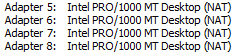
\includegraphics[width=0.5\textwidth]{Bilder/adapter}
 	\captionsetup{justification=centering}
 	\caption{VirtualBox NAT-Adapter}
	\label{adapter}
\end{wrapfigure}

Um den Hosts der Lokationen den Internetzugang zu ermöglichen, muss zuerst den Routern der Zugang zum Internet möglich sein. Dafür wurde in VirtualBox die vier Netzwerk-Adapter für die vier vorgesehenen Lokationen aktiviert und als NAT konfiguriert (siehe Abbildung \ref{adapter}). 
Die vier Schnittstellen wurden jeweils an die Router r1, r2, r3 und r4 per \textit{\textbf{Intf(„Schnittstellenbezeichnung“, node=Router-Objekt)}} Befehl zugewiesen. Die Schnittstellenbezeichnung kann vorher mit dem Befehl \textit{\textbf{ifconfig -a}} angezeigt werden. Die Router-Objekte werden vorher per \textit{\textbf{variabel = net.getNodeByName('Router-Bezeichnung')}} Befehl instanziiert. Jeder Router bekommt eine individuelle Schnittstelle zugewiesen. Die Router führen anschließend den \textit{\textbf{info(net['Router-Bezeichnung].cmd("dhclient Schnittstellenbezeichnung"))}} Befehl aus, um eine IPv4-Adresse des VirtualBox NAT-Services zu erhalten (siehe Abbildung \ref{interface}). Der IPv4-Adressenbereich, der vom NAT-Service vergeben wird, liegt bei \textit{\textbf{10.0.X.X/24}} und ändert sich je nach virtueller Maschine \cite{NATing} \cite{NATgateway}.

\begin{figure}[H]
 \centering
 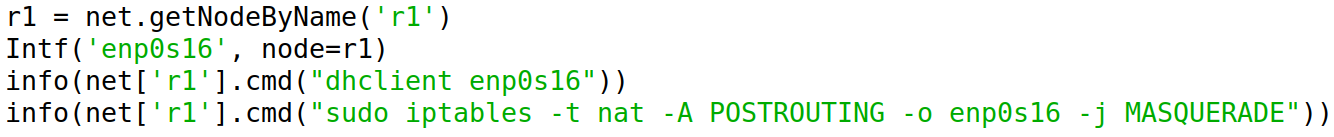
\includegraphics[width=1.0\textwidth]{Bilder/interface}
 \captionsetup{justification=centering,margin=2cm}
 \caption{Einbindung und Konfigurierung des NAT-Adapters}
 \label{interface}
\end{figure}

Da nun eine Internetverbindung für alle Router besteht, muss der Domain Name System Server auf dem Ubuntu-Host festgelegt werden, damit die Hosts nicht nur per IPv4 auf das Internet zugreifen können. Eine Möglichkeit besteht darin, die Datei \textit{\textbf{/etc/resolv.conf}} per Admin-Rechte zu bearbeiten und dort den Domain Name System Server festzulegen. Es kann der Domain Name Server von Google mit der IPv4 \textit{\textbf{8.8.8.8}} und/oder \textit{\textbf{8.8.4.4}} eingetragen werden. Ein Nachteil bei dieser Variante ist, dass nach jedem Neustart des Betriebssystems dieser Vorgang erneut durchgeführt werden muss, da der Eintrag nur temporär bis zum Ausschalten des Betriebssystems erhalten bleibt. Um dem entgegenzuwirken wurde das Paket Resolvconf per \textit{\textbf{sudo apt install resolvconf}} installiert \cite{resolvconf}. Dadurch wurden neue Dateien in der Konfigurationsebene von Ubuntu erstellt, wodurch ein permanenter Eintrag des DNS-Servers möglich war. Dafür wurde die IPv4 des DNS Server in die Datei \textit{\textbf{/etc/resolvconf/resolv.conf.d/head}} eingetragen und gespeichert. Anschließend wurde der Netzwerkmanager per \textit{\textbf{sudo systemctl restart network-manager}} Befehl neu gestartet, um die Einstellungen zu übernehmen. Jetzt ist es den Routern möglich, das Internet auch per Domainnamen zu erreichen \cite{nameservers}.

Die Default-Route der Hosts ist der jeweilige Router in der Lokation. Wenn ein Host eine Website aufruft, schickt er eine Anfrage an und über den Router. Im Moment wird die Anfrage beim Router fallengelassen, da der Router noch keine Regeln bezüglich solcher Anfragen besitzt. Die Regel wird über das im Ubuntu vorhandene Programm \textit{\textbf{iptables}} eingetragen, welches den Linux-Kernel umkonfiguriert \cite{iptables}. Dazu wird auf allen Routern der Befehl \textit{\textbf{sudo iptables -t nat -A POSTROUTING -o Schnittstellenbezeichnung -j MASQUERADE}} ausgeführt. Der Befehl vergibt jedem eingehenden Paket als Quelladresse die IPv4-Adresse der NAT-Schnittstelle des Routers \cite{iptablesmas} (siehe Abbildung \ref{adapter}). Es wird \textit{\textbf{MASQUERADE}} genutzt, weil zum Zeitpunkt der Ausführung des Befehls die IPv4-Adresse der Schnittstelle unbekannt sein beziehungsweise sich ändern kann. Bei einer statischen IPv4-Adresse der NAT-Schnittstelle würde statt MASQUERADE direkt die IP eingegeben werden \cite{iptablesnat}.
\newpage
\subsection{Ergebnis}
{\tiny Verfasst von: Mücahit\par}
Zusammenfassend wurde die NAT-Firewall-Funktion an allen Lokationen konfiguriert. Den Hosts ist es nun möglich, Anfragen ins Internet zu versenden. Der Router führt die Anfragen mit der von VirtualBox zur Verfügung gestellten Schnittstelle aus und gibt dem Host die Antwort zurück (siehe Abbildung \ref{nat}).

\begin{figure}[H]
 \centering
 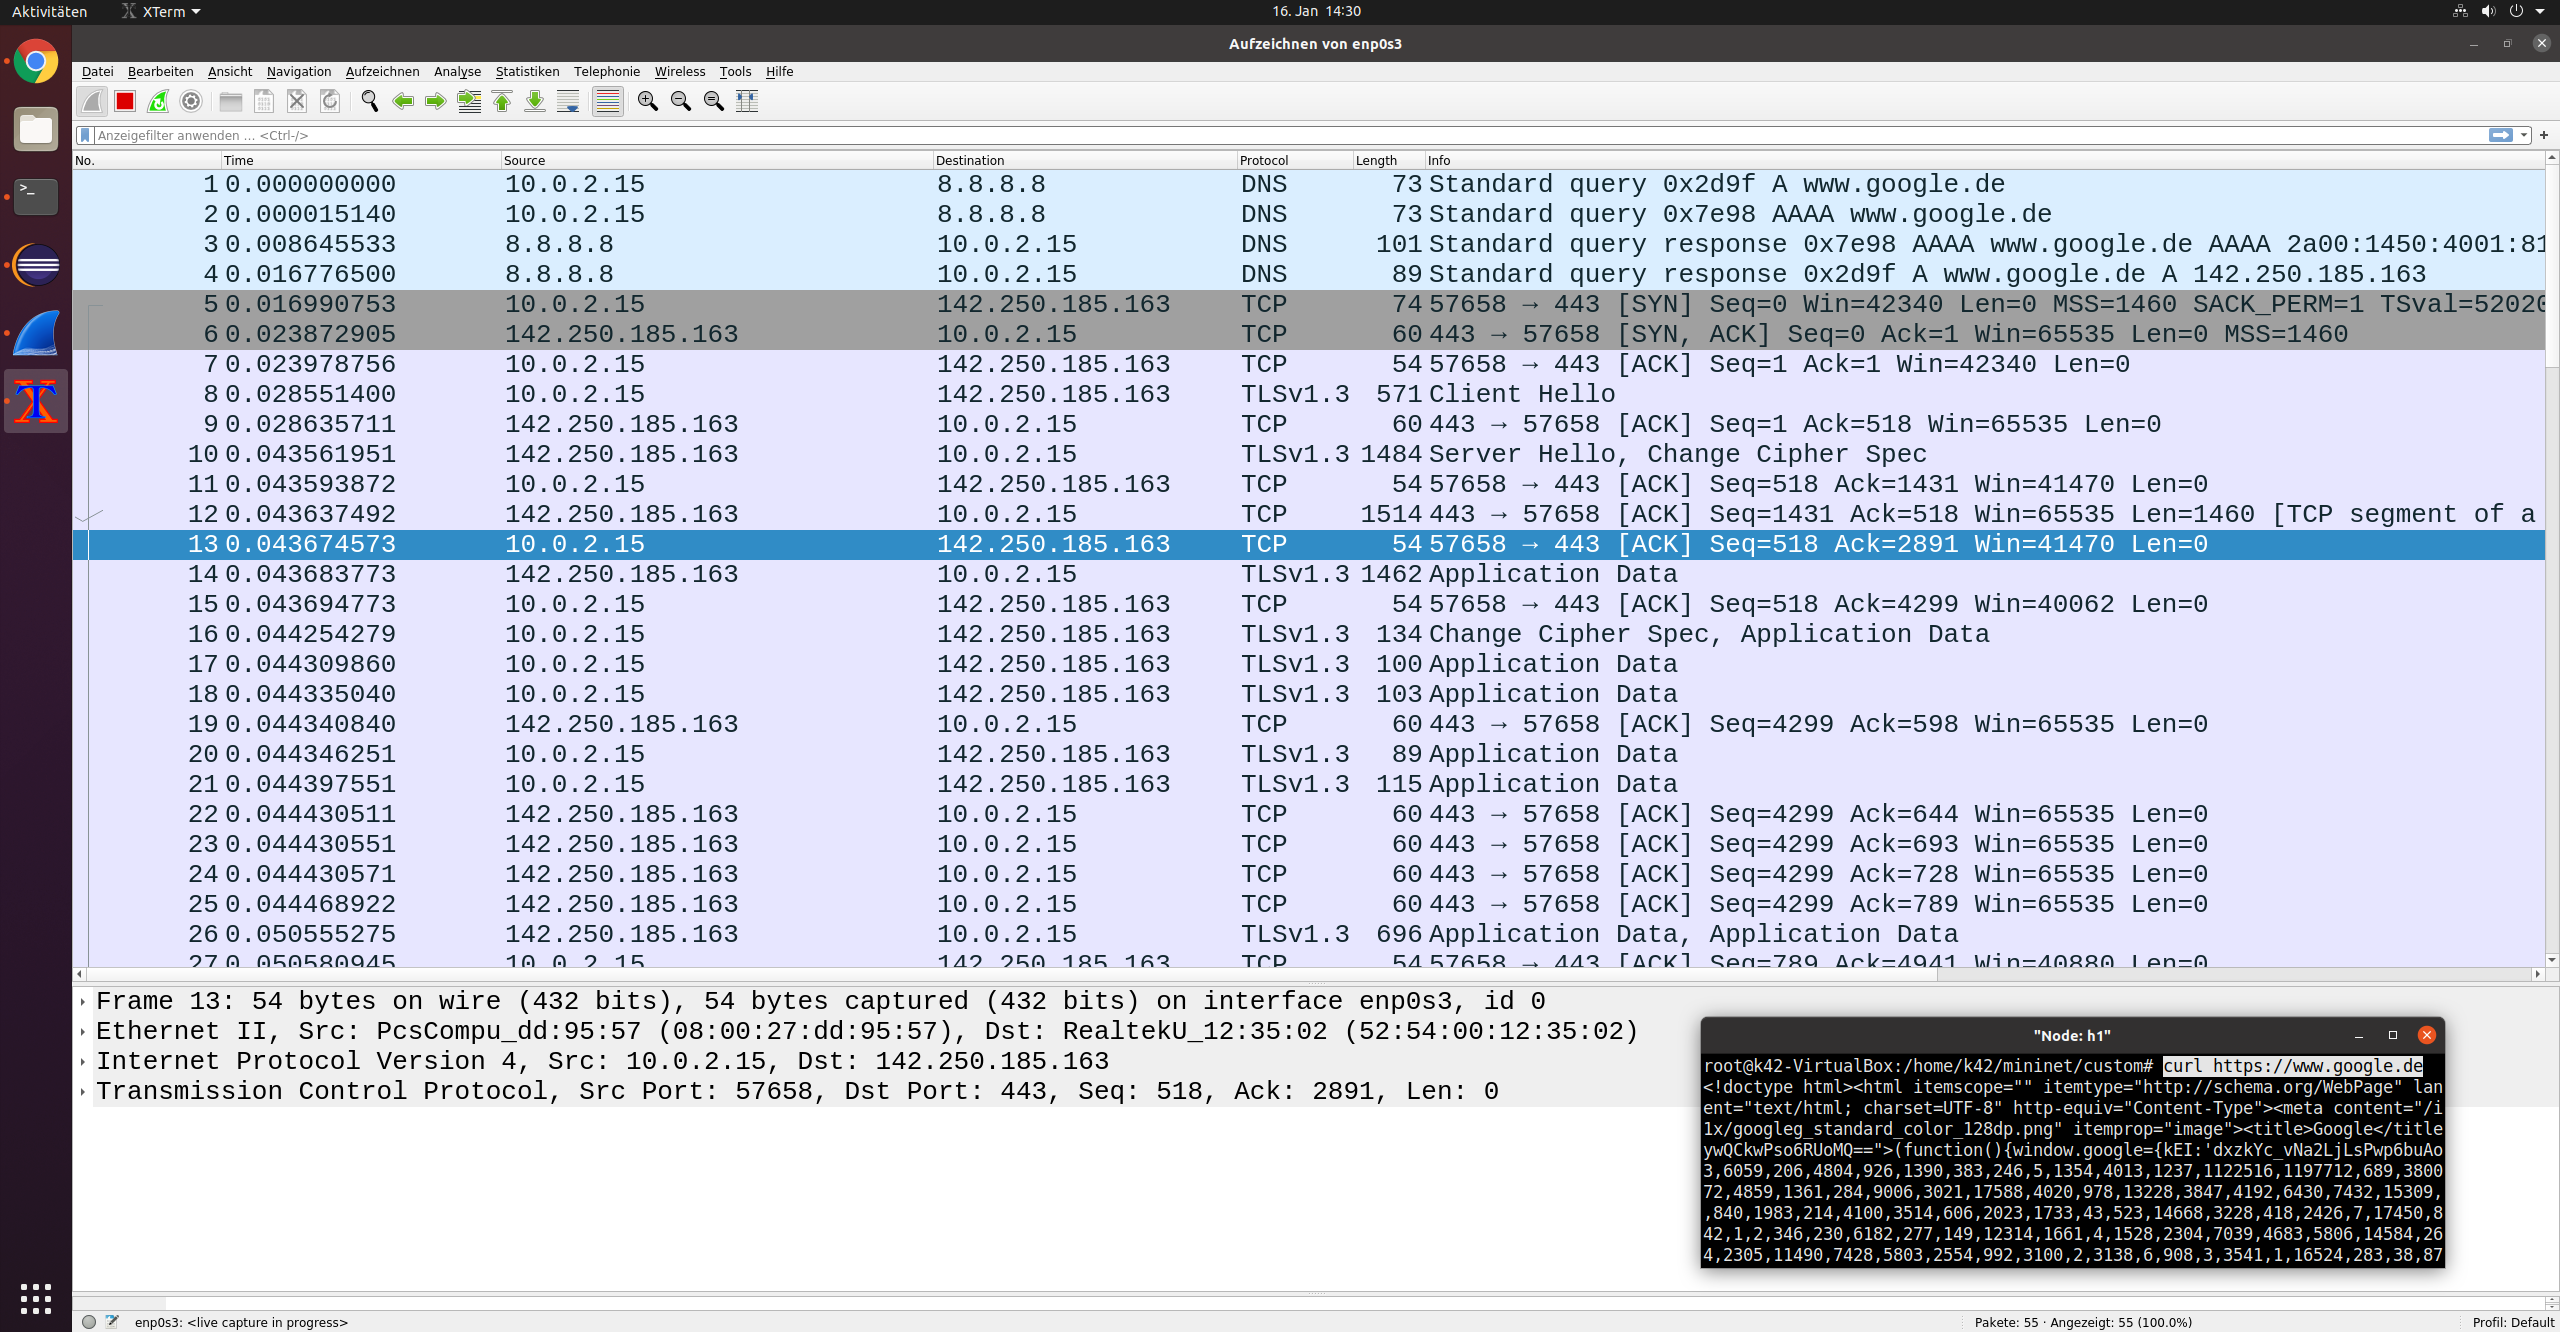
\includegraphics[width=1.0\textwidth]{Bilder/nat}
 \captionsetup{justification=centering}
 \caption{Anfrage von H1 wird über Public IP des Routers durchgeführt}
 \label{nat}
\end{figure}

Ein Problem bei der Durchführung war, dass die Netzwerkschnittstellen beim Beenden von Mininet auch für Ubuntu nicht mehr verfügbar waren. Deshalb musste immer wieder die virtuelle Maschine beziehungsweise Ubuntu neu gestartet werden, wenn Mininet beendet wurde. Um dem entgegenzuwirken, wurde der Befehl \textit{\textbf{ip link set Schnittstellenbezeichnung netns 1}} im Mininet-Script kurz vor dem Beenden eingefügt, damit die Schnittstelle erneut für Ubuntu verfügbar war.

\newpage
\section{Implementierung der Webproxy-Funktion}
{\tiny Verfasst von: Tung, Naghmeh, James, Mücahit\par}
Der Proxy übernimmt jede Hypertext Transfer Protocol (HTTP) und Hypertext Transfer Protocol Secure (HTTPS) Anfrage der Hosts, führt sie selber durch und leitet die Antwort dem ursprünglichen Host wieder zurück. Der Vorteil hierbei ist, dass der Web-Proxy-Server für eine Sicherheit in allen Schichten des OSI-Modells sorgen kann. Es muss lediglich nur an dem Web-Proxy-Server Einstellungen bezüglich gewünschter Inhalte, IP-Adressen oder MAC-Adressen vorgenommen werden. Damit ist die Sicherheit für alle Geräte gewährleistet, die über den Web-Proxy-Server Anfragen verschicken. Des Weiteren wäre die Bandbreite weniger ausgelastet, da der Web-Proxy-Server jede neue Antwort in seinem Cache speichert. Bei gleicher Anfrage in einem benutzerdefinierten Zeitintervall wird die Antwort aus dem Cache statt durch erneute Anfrage ins Internet ausgegeben \cite{webproxyosi}.

\subsection{Vorüberlegung}
{\tiny Verfasst von: Tung, Naghmeh, James, Mücahit\par}
Für eine Webproxy-Funktion muss in allen Lokationen ein Webproxy-Server eingerichtet werden. Hosts müssen ohne vorher konfiguriert zu werden, Anfragen über den Proxy versenden können, wenn sie neu an das Netzwerk hinzukommen. Dem Host ist nicht bewusst, dass seine Anfragen über einen Proxy laufen. Anfragen würden über den Switch an den Webproxy weitergeleitet werden. Dieser führt die Anfrage durch und gibt dem Host die Antwort zurück. Die Umleitung sollte durch den Controller konfiguriert werden. 

\subsection{Durchführung}
{\tiny Verfasst von: Tung, Naghmeh, James, Mücahit\par}
Um die Webproxy-Funktion zu realisieren, wurde in allen Lokationen jeweils ein weiterer Host in Mininet konfiguriert. Es wurde allen eine IPv4-Adresse im jeweiligen privaten Netzwerkadressenbereich vergeben und mit dem dazugehörigen Switch verbunden. Diese Hosts sollen nun als Webproxy-Server dienen. Es wurde zunächst per \textit{\textbf{Xterm Proxybezeichnung}} Befehl ein externes Terminal gestartet und die Internetverbindung durch das Aufrufen einer beliebigen Website als funktionsfähig getestet. Dazu wurde das Kommandozeilenprogramm \textit{\textbf{cURL}} verwendet, welcher vorher per \textit{\textbf{sudo apt install curl}} installiert werden muss.
Als Nächstes sollte eine weitere Schnittstelle des Webproxy-Servers mit einer Schnittstelle von VirtualBox verbunden werden. Dieser sollte dann als Bridge zwischen zwei VirtualBox-Maschinen genutzt werden. Auf der zweiten VirtualBox-Maschine sollte das Programm Squid installiert werden. Im Gesamtbild sollte eine Anfrage eines Hosts über den Proxy-Server-Host auf eine andere VirtualBox-Maschine weitergeleitet, dort durchgeführt und die Antwort anschließend zurückgeleitet werden. Leider scheiterte dieser Versuch, da bei der Haupt-VirtualBox-Maschine der Promiscuous-Modus des Netzwerkbrückenadapters auf deny eingestellt war. Dadurch kam keine Verbindung zwischen den zwei VirtualBox-Maschinen zustande. Aus diesem Grund wurde ein alternativer Proxy-Skript aus Github benutzt, um die Webproxy-Funktionalität direkt auf dem Host beziehungsweise Server einzurichten. Dazu wurde per Xterm ein Host-Terminal gestartet und das Skript ausgeführt. Dieser nimmt nur HTTP Anfragen entgegen, führt sie selber durch und gibt für einen bestimmtes Zeitintervall die Antworten aus dem Cache zurück. Hier ist noch mal zu verdeutlichen, dass das Python-Skript für keine umfangreiche Web-Proxy-Funktionalität ausgelegt ist, jedoch dieser aus Testzwecken benutzt wurde. Als Nächstes wurden alle Pakete, die beim Switch eingehen und einen Ziel-Port als 80 besitzen, an den Proxy weitergeleitet. Hierfür wurde über den Controller die entsprechenden Flows als Match eingetragen, die dazugehörigen Actions implementiert und dem Switch die Anweisungen geschrieben. Dadurch bekommt der Webproxy-Server die Anfragen der Hosts, ohne dass die Geräte umkonfiguriert werden müssen. Der Proxy nimmt die Anfrage entgegen, führt sie selber durch und gibt die Antwort an das jeweilige Gerät weiter. Hier tritt das Problem auf, dass das Gerät eine Antwort von der Website erwartet, jedoch die Antwort vom Proxy geschickt bekommt. Die Antwort des Proxys könnte ebenfalls per Controller modifiziert und an das jeweilige Gerät weitergeleitet werden. Jedoch fehlte die Information des Absenders aus dem Internet zu dem Zeitpunkt, an dem die Antwort vom Proxy an den Host geschickt wurde.

\subsection{Ergebnis}
{\tiny Verfasst von: Tung, Naghmeh, James, Mücahit\par}
Resultierend war es nicht möglich, die Webproxy-Funktion zu implementieren. Alternativ könnte eine transparente Web-Proxy-Funktion an dem Router der jeweiligen Lokationen eingerichtet werden. Dieser führt die Anfragen selber durch, speichert und sendet die Antwort an den jeweiligen Host zurück. Auch das Eintragen des Proxyservers an den jeweiligen Hosts, die mit dem Switch verbunden sind, würde sich als funktionsfähig erweisen. Diese Art wird direkter Proxy genannt und trägt viel Aufwand mit sich \cite{webproxy}.

\newpage
\section{Aufbau eines zentralen Topologie-Viewers und einer Monitoring-Lösung}

\subsection{Topologie}
{\tiny Verfasst von: Mücahit\par}
Die Topologie unseres Netzwerkes kann auf dem Web User Interface des Floodlight-Controllers eingesehen werden. Ein mit der Standardinstallation geliefertes Floodlight-Modul stellt die Information der Topologie in einer Weboberfläche zur Verfügung. Zum Einsehen der Topologie muss auf einem Webbrowser die Benutzeroberfläche des Controllers über den Link \textit{\textbf{http://<controller-ip>:8080/ui/index.html}} aufgerufen werden \cite{restapi}. Anschließend wird auf dem linken Reiter die Option Topology angeklickt, wodurch die Topologie angezeigt wird (siehe Abbildung \ref{topo}). Durch die Benutzung einer VirtualBox werden vier getrennte Topologien angezeigt. Die Verbindungen zwischen den Routern werden bei der Visualisierung vom Controller ignoriert. Dies schränkt jedoch nicht die Funktionsweise des Netzwerkes ein. Bei der Nutzung vier getrennter VirtualBox-Maschinen, würde die Topologie korrekt dargestellt werden.

\begin{figure}[H]
 \centering
 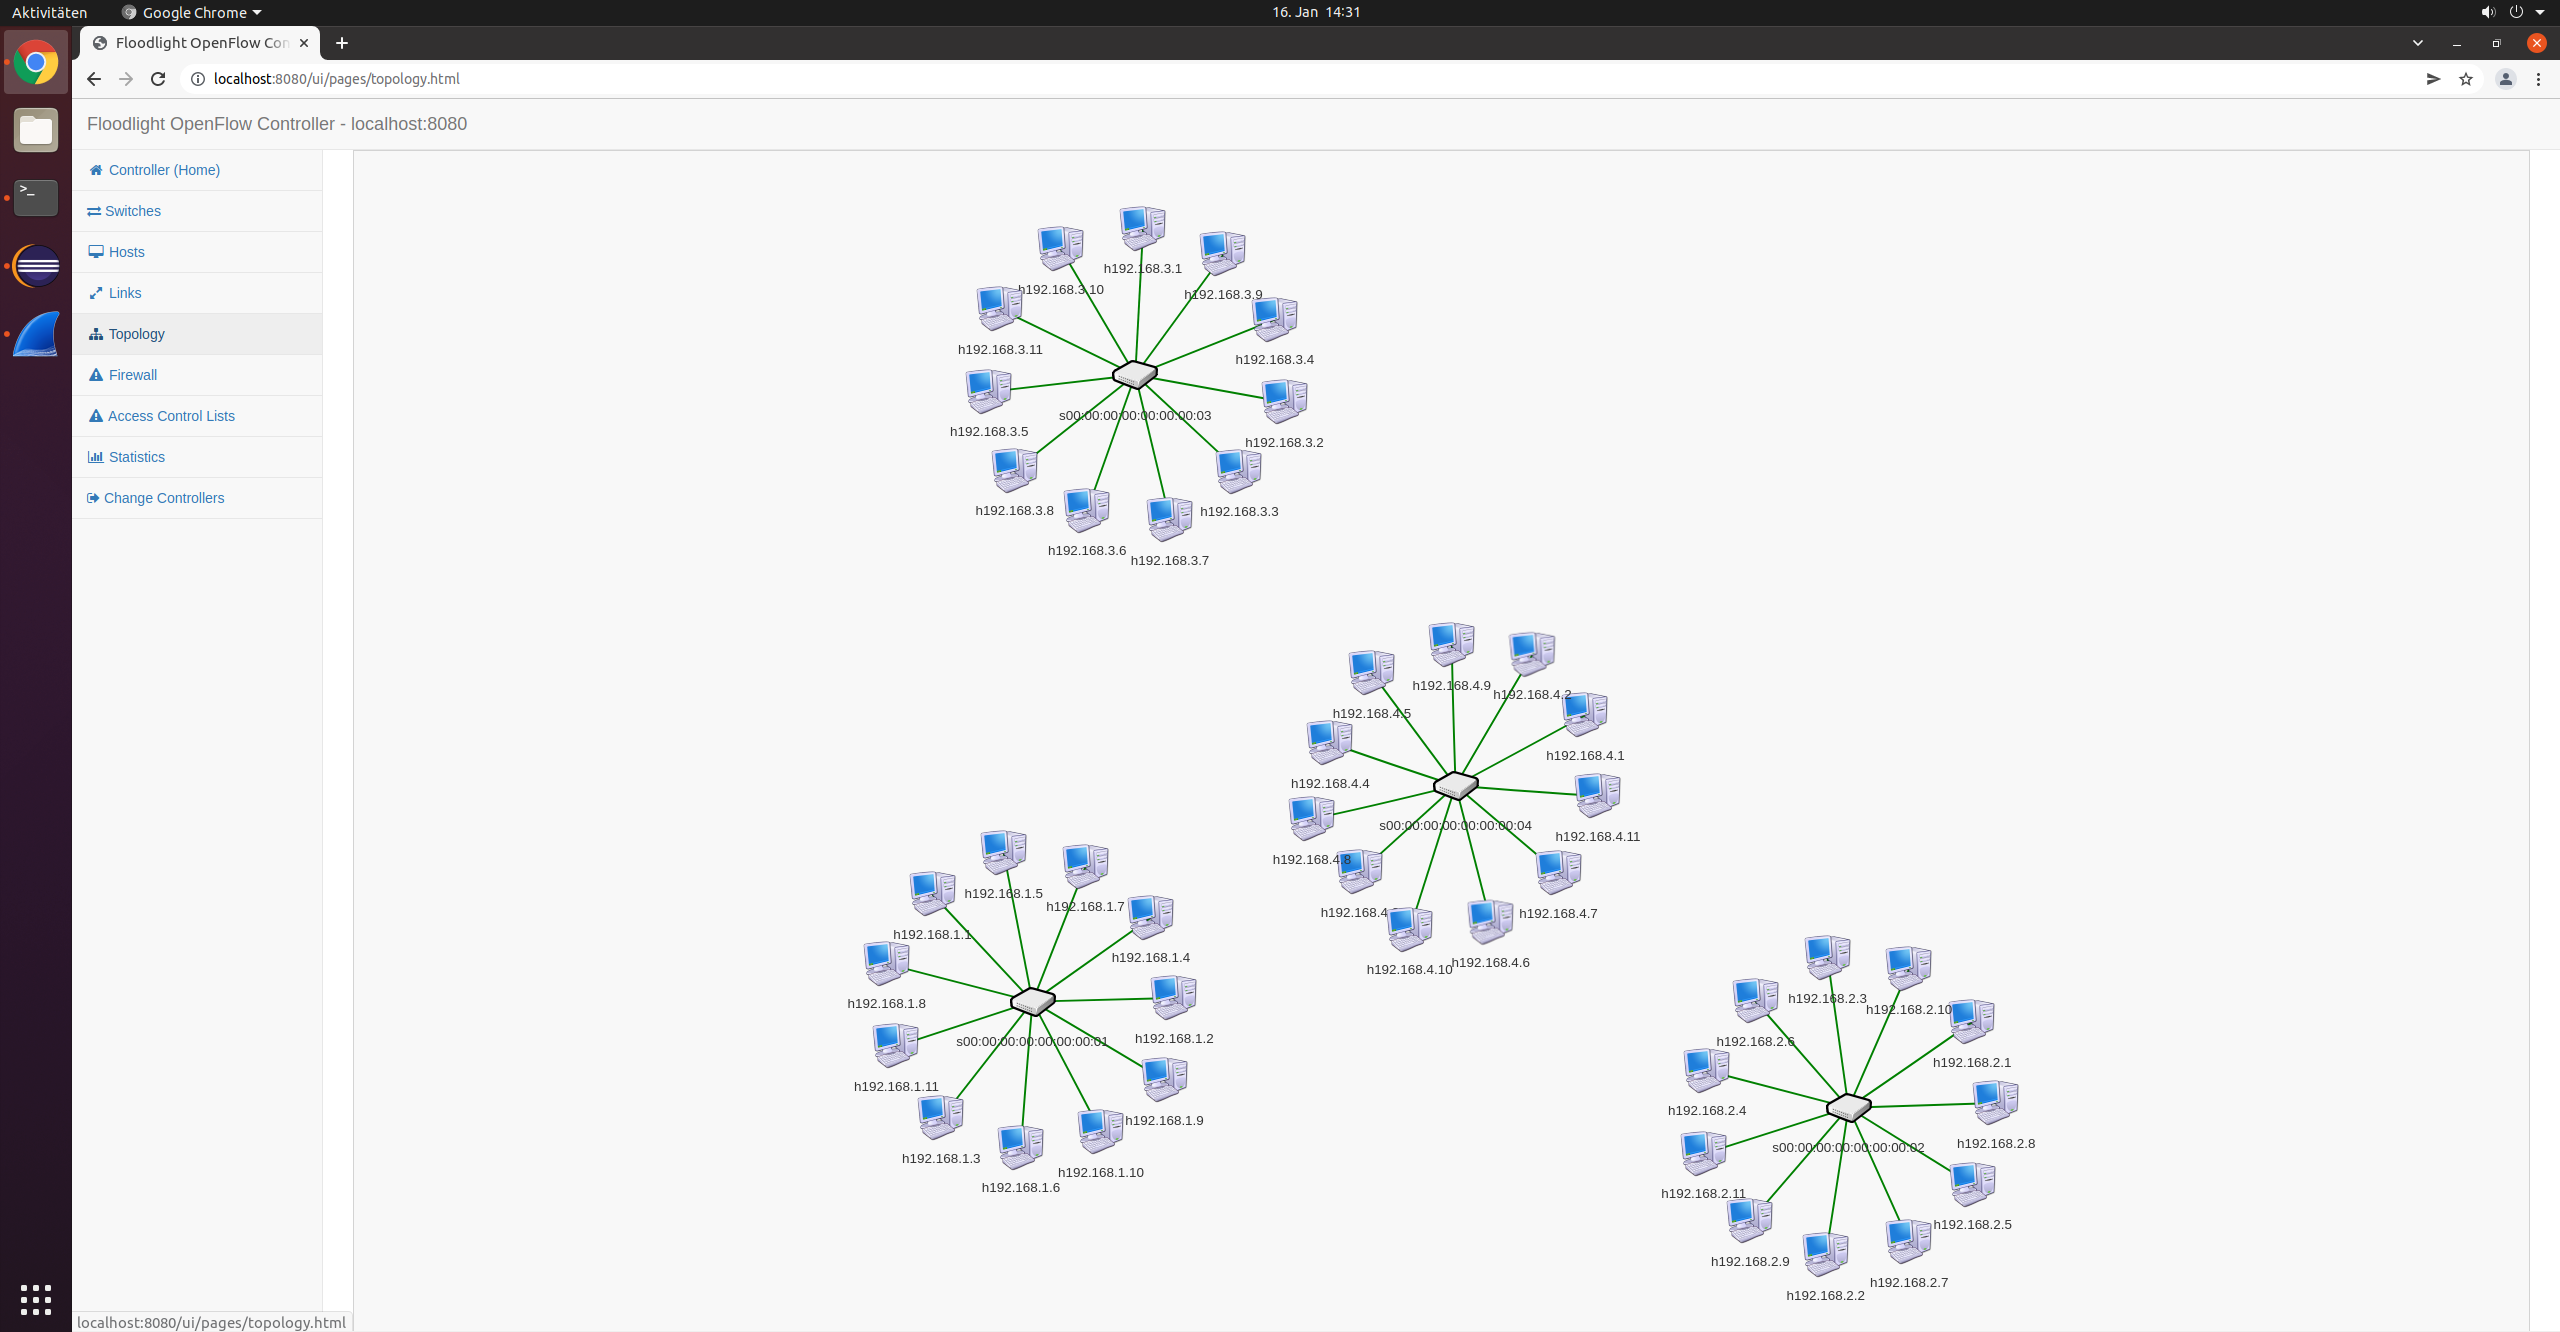
\includegraphics[width=1.0\textwidth]{Bilder/topo}
 \captionsetup{justification=centering}
 \caption{Topologie des Netzwerkes auf der Webbenutzeroberfläche von Floodlight}
 \label{topo}
\end{figure}

\newpage
\subsection{Monitoring-Lösung}
{\tiny Verfasst von: Mücahit\par}
Für das zentrale Monitoring wird Nagios Core zum Einsatz kommen. Es kann auf einer großen Anzahl an Umgebungen installiert werden. Die Software bietet eine Weboberfläche, die von allen Netzwerkteilnehmern erreicht werden kann. Dabei kann die Verfügbarkeit, Geschwindigkeit und Dienste der Netzwerkkomponenten überprüft werden. Bei entstehenden Fehlern können Administratoren benachrichtigt werden, um die Fehler zu beheben. Bei großen Netzwerken spielt dies eine wichtige Rolle, da die Verfügbarkeit bei kritischen Anwendungen von großer Bedeutung ist \cite{nagiosdef}.\par
Zunächst wird Nagios Core auf der VirtualBox-Maschine installiert, wo auch Mininet und Floodlight laufen. Bis jetzt lief Floodlight auf dem localhost, also der \textit{\textbf{127.0.0.1}} IP, welches nun geändert werden muss damit die Netzwerkteilnehmer auf die Floodlight REST-API und im Moment wichtiger auf den Nagios Core Dienst zugreifen können. Dafür werden im Mininet-Skript Befehle eingefügt, um den Switches 1-4 eine IP-Adresse zuzuweisen (siehe Abbildung \ref{switch}). Ebenfalls wird die Default-Route als \textit{\textbf{192.168.1.1}} hinzugefügt, da Nagios Core auf der IP \textit{\textbf{192.168.1.20}} laufen wird. Der Controller wurde auch konfiguriert auf dieser IP zu laufen. Nagios Core und der Controller sind nun von allen Netzwerkteilnehmern erreichbar.

\begin{figure}[H]
 \centering
 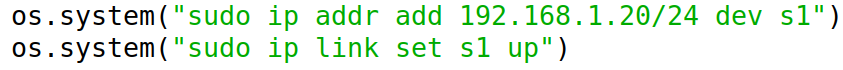
\includegraphics[width=0.7\textwidth]{Bilder/switch}
 \captionsetup{justification=centering, margin=2cm}
 \caption{Hinzufügen der Switch IP für s1}
 \label{switch}
\end{figure}
 
Die Installation von Nagios Core findet auf der Haupt-VirtualBox-Maschine statt und wird Schritt für Schritt erklärt. Die Befehle sollten nacheinander im Linux-Terminal ausgeführt werden.

\newlength\myboxwidth

\setlength{\myboxwidth}{\dimexpr\textwidth-2\fboxsep}

\begin{itemize}
\item[1.] Das Betriebssystem auf den neuesten Stand bringen
\end{itemize}
\colorbox{CadetBlue}{\textcolor{white}{\textbf{\textsf{\$ sudo apt update \& \& upgrade -y}}}}
\begin{itemize}
\item[2.] Alle benötigten Abhängigkeiten installieren
\end{itemize}
\colorbox{CadetBlue}{\parbox{\myboxwidth}{\textbf{\textsf{\textcolor{white}{\$ sudo apt install \hyp{}y build\hyp{}essential apache2 php openssl perl makephp\hyp{}gd libgd\hyp{}dev libapache2\hyp{}mod\hyp{}php libperl\hyp{}dev libssl\hyp{}dev daemonwget apache2\hyp{}utils unzip}}}}}
\begin{itemize}
\item[3.] Nagios Benutzer und Gruppe hinzufügen
\end{itemize}
\colorbox{CadetBlue}{\textcolor{white}{\textbf{\textsf{\$ sudo useradd nagios}}}}\\
\colorbox{CadetBlue}{\textcolor{white}{\textbf{\textsf{\$ sudo groupadd nagcmd}}}}\\
\colorbox{CadetBlue}{\textcolor{white}{\textbf{\textsf{\$ sudo usermod -a -G nagcmd nagios}}}}\\
\colorbox{CadetBlue}{\textcolor{white}{\textbf{\textsf{\$ sudo usermod -a -G nagcmd www-data}}}}
\begin{itemize}
\item[4.] Nagios in einen beliebigen Ordner herunterladen
\end{itemize}
\colorbox{CadetBlue}{\parbox{\myboxwidth}{\textbf{\textsf{\textcolor{white}{\$ wget https://assets.nagios.com/downloads/nagioscore/releases/nagios-4.4.5.tar.gz}}}}}
\begin{itemize}
\item[5.] Die Datei extrahieren und in den Ordner wechseln
\end{itemize}
\colorbox{CadetBlue}{\textcolor{white}{\textbf{\textsf{\$ tar -zxvf /tmp/nagios-4.4.5.tar.gz}}}}\\
\colorbox{CadetBlue}{\textcolor{white}{\textbf{\textsf{\$ cd /nagios-4.4.5/}}}}
\begin{itemize}
\item[6.] Nagios einstellen (hierbei wird der Benutzer und die Gruppe angegeben)
\end{itemize}
\colorbox{CadetBlue}{\parbox{\myboxwidth}{\textbf{\textsf{\textcolor{white}{\$ sudo ./configure --with-nagios-group=nagios--with-command-group=nagcmd --with-httpd\_conf=/etc/apache2/sites-enabled/}}}}}
\begin{itemize}
\item[7.] Die Dateien vorbereiten und installieren
\end{itemize}
\colorbox{CadetBlue}{\textcolor{white}{\textbf{\textsf{\$ sudo make all}}}}\\
\colorbox{CadetBlue}{\textcolor{white}{\textbf{\textsf{\$ sudo make install}}}}\\
\colorbox{CadetBlue}{\textcolor{white}{\textbf{\textsf{\$ sudo make install-init}}}}\\
\colorbox{CadetBlue}{\textcolor{white}{\textbf{\textsf{\$ sudo make install-config}}}}\\
\colorbox{CadetBlue}{\textcolor{white}{\textbf{\textsf{\$ sudo make install-commandmode}}}}
\begin{itemize}
\item[8.] Optional: Kontaktdaten in die contacts.cfg einfügen, um Notifications zu erhalten
\end{itemize}
\colorbox{CadetBlue}{\textcolor{white}{\textbf{\textsf{\$ sudo gedit /usr/local/nagios/etc/objects/contacts.cfg}}}}
\begin{itemize}
\item[9.] Webinterface installieren und Module aktivieren
\end{itemize}
\colorbox{CadetBlue}{\textcolor{white}{\textbf{\textsf{\$ sudo make install-webconf}}}}\\
\colorbox{CadetBlue}{\textcolor{white}{\textbf{\textsf{\$ sudo a2enmod cgi}}}}
\begin{itemize}
\item[10.] Nagios-Benutzer erstellen
\end{itemize}
\colorbox{CadetBlue}{\textcolor{white}{\textbf{\textsf{\$ sudo htpasswd -c /usr/local/nagios/etc/htpasswd.users nagiosadmin}}}}
\begin{itemize}
\item[11.] Webserver neustarten
\end{itemize}
\colorbox{CadetBlue}{\textcolor{white}{\textbf{\textsf{\$ sudo systemctl restart apache2}}}}
\begin{itemize}
\item[12.] Optional: Nagios Plugins herunterladen und installieren
\end{itemize}
\colorbox{CadetBlue}{\textcolor{white}{\textbf{\textsf{\$ wget https://nagios-plugins.org/download/nagios-plugins-2.3.3.tar.gz}}}}\\
\colorbox{CadetBlue}{\textcolor{white}{\textbf{\textsf{\$ tar -zxvf /tmp/nagios-plugins-2.3.3.tar.gz}}}}\\
\colorbox{CadetBlue}{\textcolor{white}{\textbf{\textsf{\$ cd /nagios-plugins-2.3.3/}}}}\\
\colorbox{CadetBlue}{\textcolor{white}{\textbf{\textsf{\$ sudo ./configure --with-nagios-user=nagios --with-nagios-group=nagios}}}}\\
\colorbox{CadetBlue}{\textcolor{white}{\textbf{\textsf{\$ sudo make}}}}\\
\colorbox{CadetBlue}{\textcolor{white}{\textbf{\textsf{\$ sudo make install}}}}
\newpage
\begin{itemize}
\item[13.] Nagios bei Systemstart starten und Nagios ausführen
\end{itemize}
\colorbox{CadetBlue}{\textcolor{white}{\textbf{\textsf{\$ sudo systemctl enable nagios}}}}\\
\colorbox{CadetBlue}{\textcolor{white}{\textbf{\textsf{\$ sudo systemctl start nagios}}}}


Mit all den Schritten wurde Nagios Core inklusive der Plugins installiert \cite{nagiosinstall}. Der Webserver von Nagios läuft nach Neustarten des Dienstes auf den IP-Adressen der Switches. Dazu muss die IP inklusive des Pfades \textit{\textbf{/nagios}} aufgerufen werden. Dort sind im Moment nur Informationen über das System, welches Nagios ausführt, enthalten. Die Netzwerkkomponenten müssen manuell in Nagios eingefügt werden. Bevor das funktioniert, muss für die Switches eine Einstellung in der \textit{\textbf{nagios.cfg}} vorgenommen werden. Dort muss die Raute vor dem \textit{\textbf{cfg\_file=/usr/local/nagios/etc/objects/switch.cfg}} Befehl entfernt werden, damit die \textit{\textbf{switch.cfg}} in Nagios mitübernommen wird. Nun werden in der \textit{\textbf{switch.cfg}} alle Switches mit der Bezeichnung, deren IP und der zugehörigen Gruppe aufgelistet (siehe Abbildung \ref{nagios-switch}). Danach können sogenannte Services für die Überwachung der Verfügbarkeit, der Geschwindigkeit und weitere Informationen hinzugefügt werden (siehe Abbildung \ref{nagios-service}). Anschließend muss der Nagios Dienst neu gestartet werden. Um Fehler zu vermeiden, sollte per \textit{\textbf{sudo /usr/local/nagios/bin/nagios -v /usr/local/nagios/etc/nagios.cfg}} Befehl geschaut werden, ob Unstimmigkeiten bei den geänderten Konfigurationen existieren \cite{nagiosrouter}.\par

\begin{figure}[H]
 \centering
 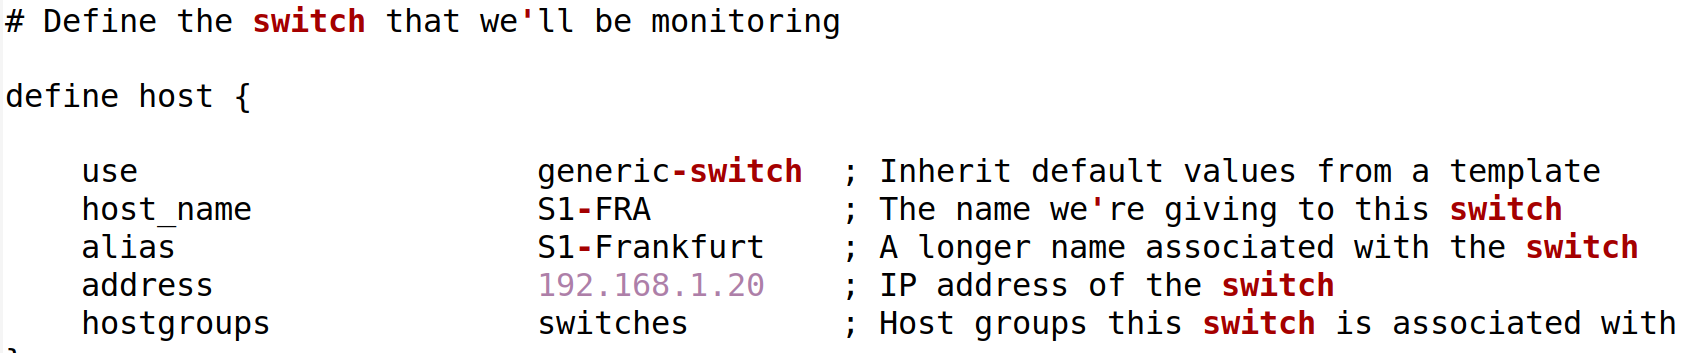
\includegraphics[width=1.0\textwidth]{Bilder/nagios-switch}
 \captionsetup{justification=centering, margin=2cm}
 \caption{Definition der Switch für Nagios}
 \label{nagios-switch}
\end{figure}

\begin{figure}[H]
 \centering
 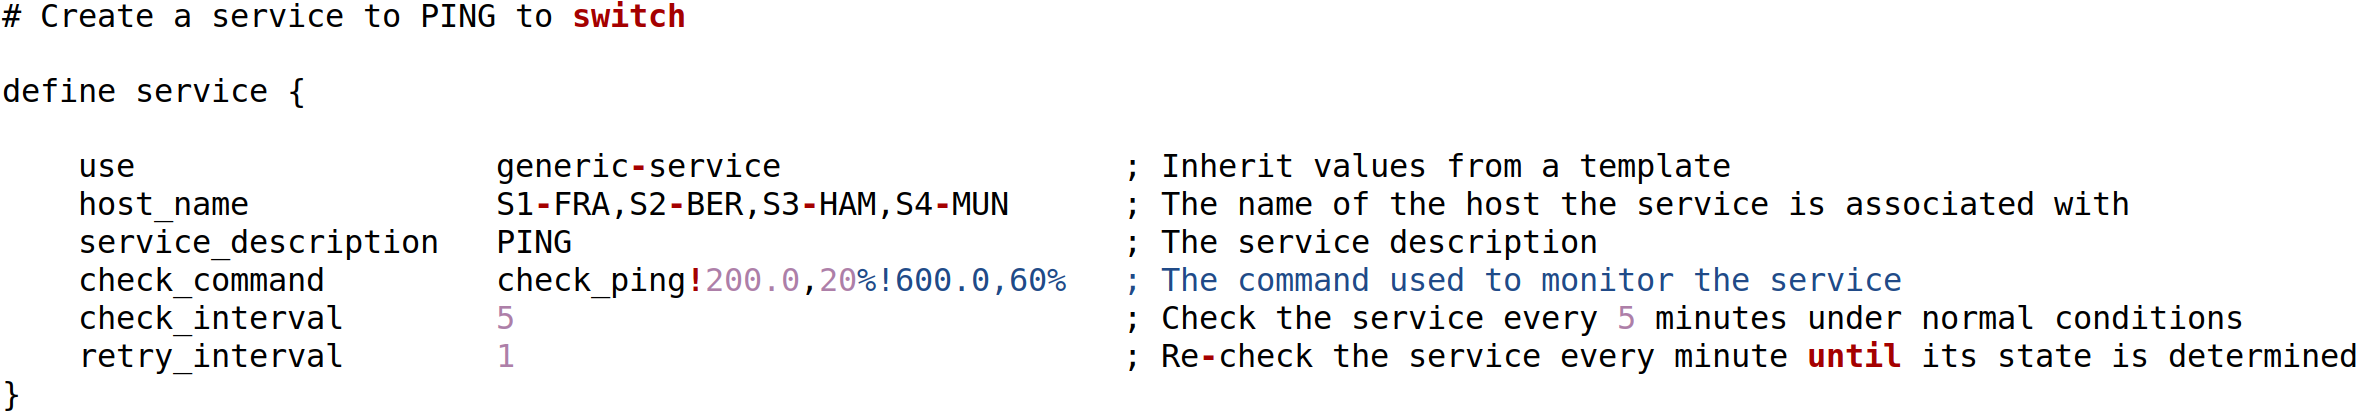
\includegraphics[width=1.0\textwidth]{Bilder/nagios-service}
 \captionsetup{justification=centering, margin=2cm}
 \caption{Definition der Services für die Switch}
 \label{nagios-service}
\end{figure}
Nachdem alle Netzwerkteilnehmer und -komponenten hinzugefügt und die gewünschten Services eingestellt worden sind, werden alle Informationen auf der Webbenutzeroberfläche angezeigt (siehe Abbildung \ref{nagios}). Unter dem Reiter Hosts kann die Verfügbarkeit aller Teilnehmer angezeigt werden. Die Verfügbarkeit kann unter mehreren Zuständen unterscheiden. Ein Host kann daher den Zustand \textit{\textbf{Up, Down, Unreachable}} und \textit{\textbf{Pending}} haben, welche auch mit Farben visualisiert werden. Unter Services werden alle Teilnehmer mit den konfigurierten Services angezeigt. Die Services haben ebenfalls Zustände. Dazu gehört unteranderem \textit{\textbf{Ok, Warning, Unknown, Critical}} und \textit{\textbf{Pending}}, die ebenfalls mit Farben visualisiert werden. Bei Host Groups werden die Teilnehmer gruppiert und die Informationen zusammengefasst angezeigt. Des Weiteren können viele weitere Einstellungen bezüglich der Benachrichtigungen und der Services über die Webbenutzeroberfläche vorgenommen werden. Dazu klickt man auf einen Teilnehmer und kann auf dem rechten Abschnitt sogenannte \textit{\textbf{Host Commands}} benutzen. Beispielsweise können Kommentare zu Hosts oder Services verfasst werden, damit andere Nutzer bestimmte Vorgänge nachvollziehen können. Zusammenfassend kann über Nagios das gesamte Netzwerk zentral überwacht werden.


\begin{figure}[H]
 \centering
 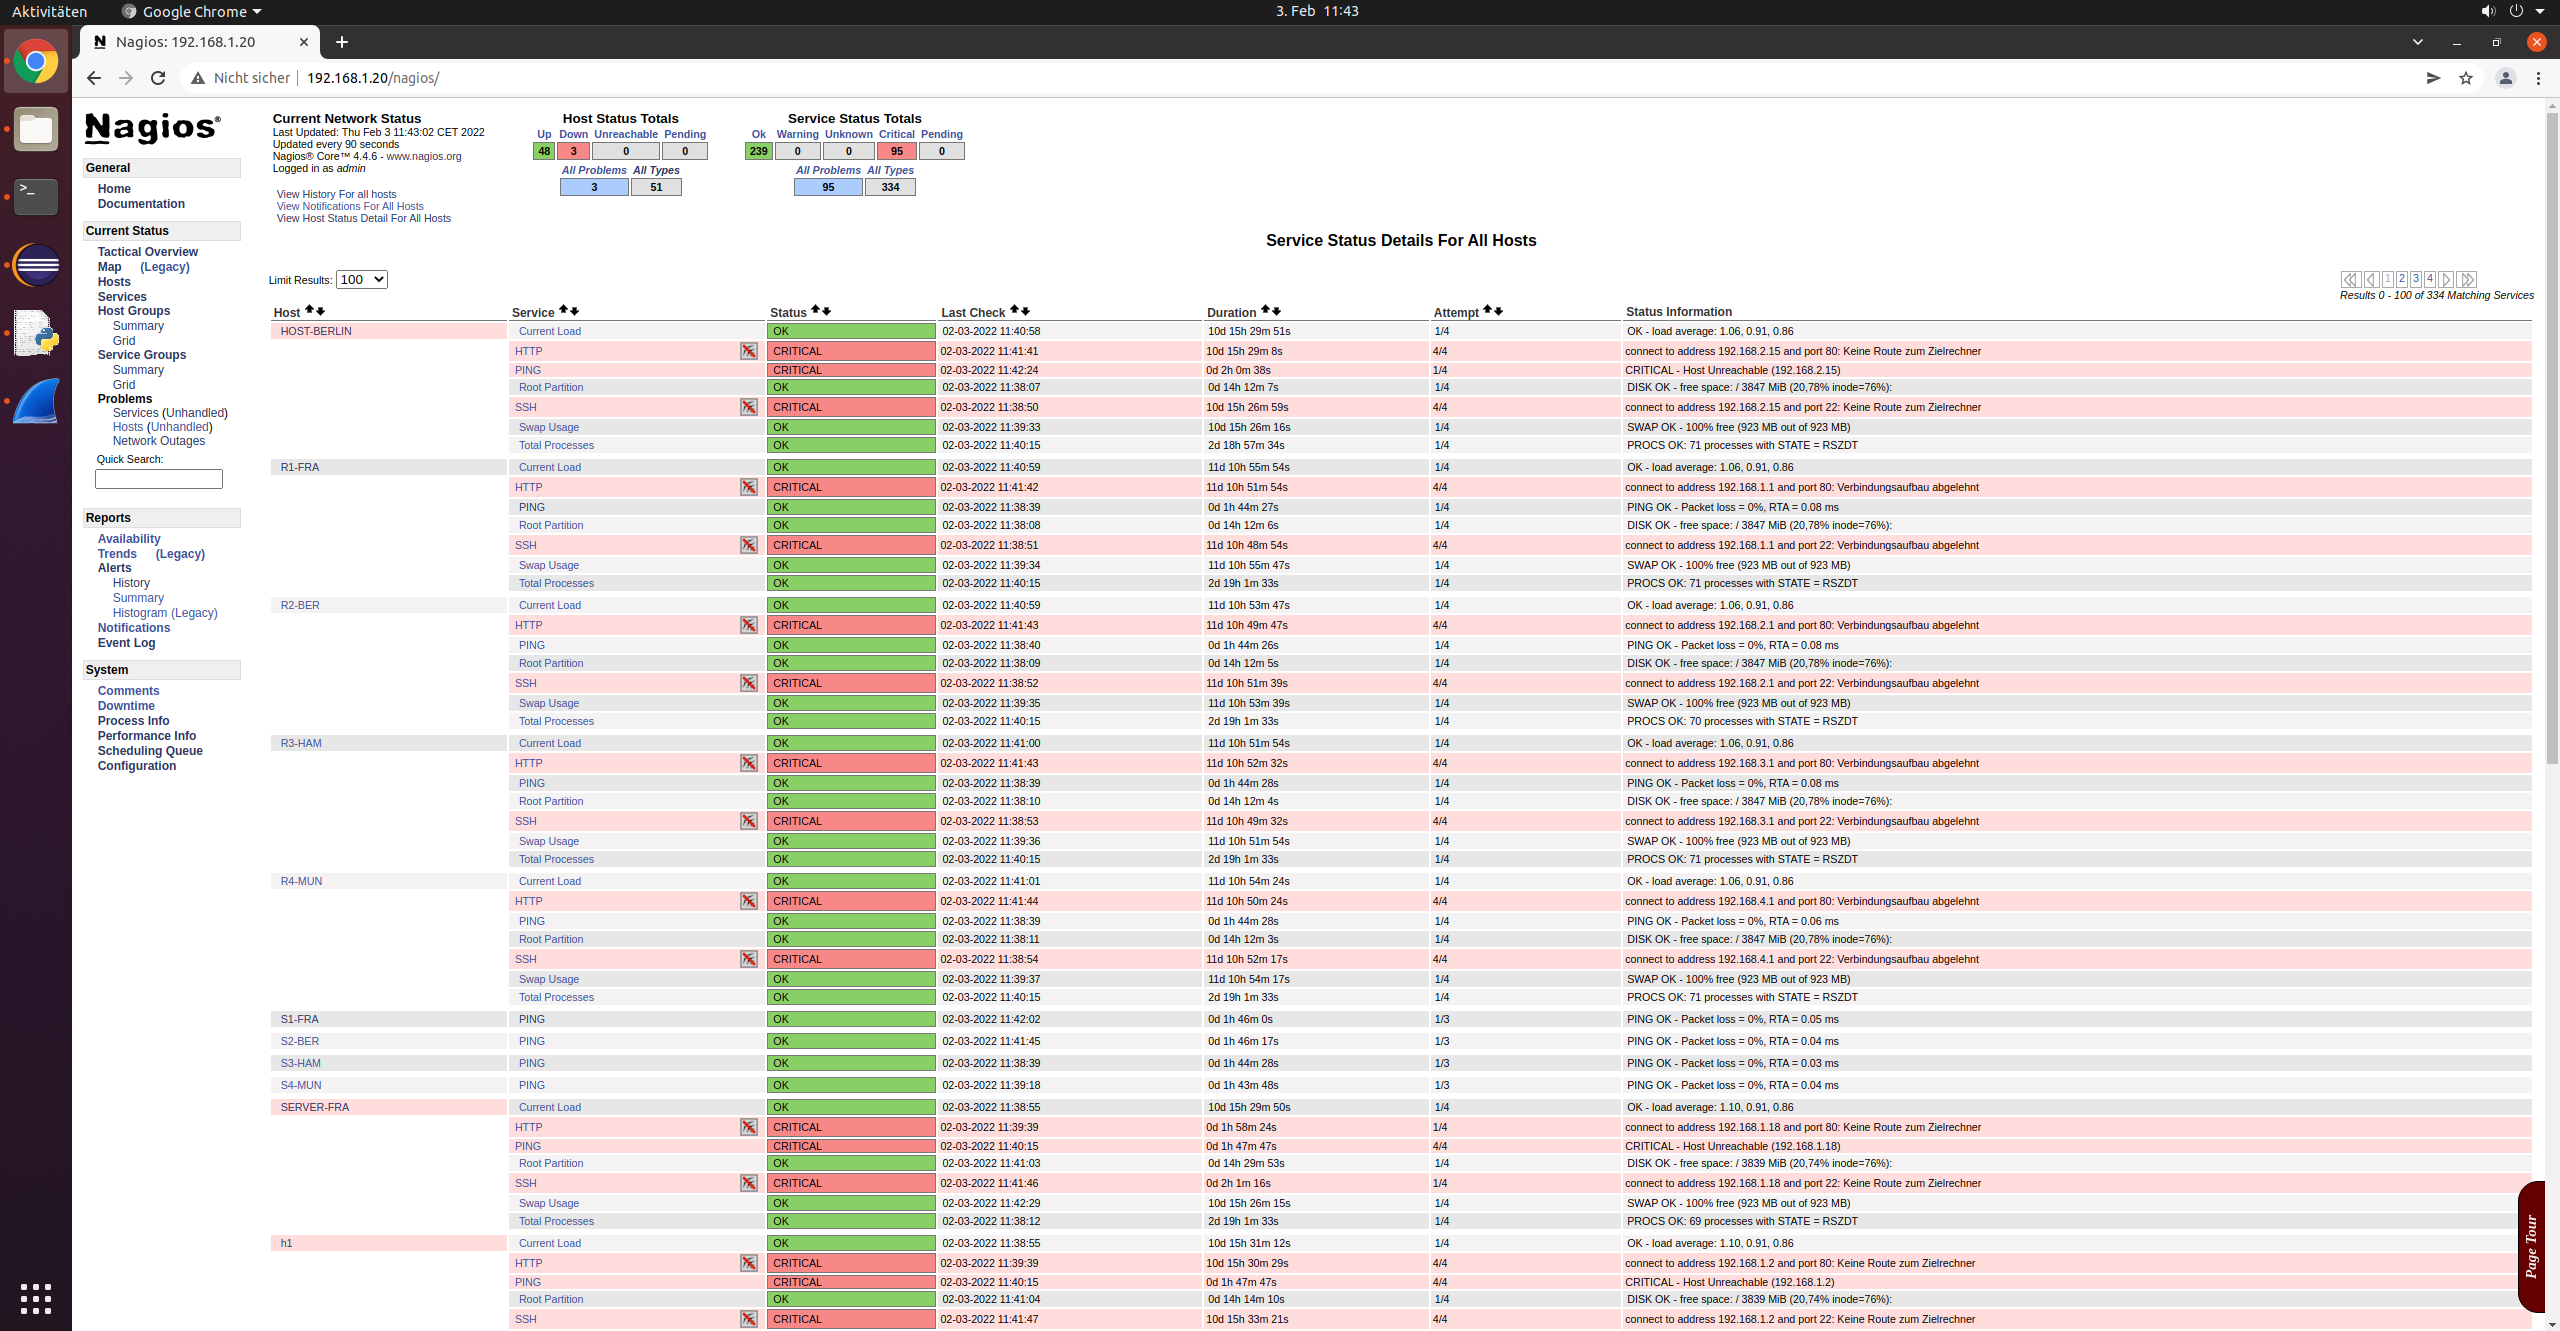
\includegraphics[width=1.0\textwidth]{Bilder/nagios}
 \captionsetup{justification=centering, margin=2cm}
 \caption{Webbenutzeroberfläche von Nagios Core}
 \label{nagios}
\end{figure}

\newpage
\section{Realisierung einer Quality of Service Funktion}
{\tiny Verfasst von: Mücahit\par}
Die Quality of Service Funktion gewährleistet die Fähigkeit des Netzwerkes, Anwendungen und Datenverkehr selbst bei begrenzter Netzwerkkapazität zuverlässig mit hoher Priorität auszuführen \cite{qosdef}. Das Netzwerkes muss für alle Audio- und Video-Konferenzen innerhalb der Lokationen genügend Bandbreite zur Verfügung stellen. Die Verbindung zwischen den Lokationen besteht aus einer Standleitung mit einer Geschwindigkeit von 20 Megabit.

\subsection{Vorüberlegung}
{\tiny Verfasst von: Mücahit\par}
Pakete, die für die Audio- und Videokonferenzen verantwortlich sind, müssen an dem Switch über den Controller priorisiert werden. Durch die Priorisierung sollen bei einer Auslastung des Netzwerkes die Audio- und Videokonferenzen stabil und flüssig laufen. Nach einer ausgiebigen Recherche kam der Entschluss, UDP Pakete zu priorisieren, da die meisten Videokonferenzprogramme wie beispielsweise Skype und Zoom diese verwenden. Zusätzlich muss getestet werden, wie viel Megabit pro Host eine ausreichende Bandbreite darstellen \cite{qosbenefits}.\par
An dem Port der Switch, der zum Router der Lokationen führt, werden zwei sogenannte Queues erstellt. Eine Queue wird für die Audio- und Videokonferenzen und die andere Queue für den restlichen Datenverkehr verwendet. Dabei erhalten die Queues Eigenschaften wie der minimalen und/oder maximalen Bandbreite zur Gewährleistung der Quality of Service \cite[952]{qosof}. Nach der Konfiguration sollte gezeigt werden, ob Pakete tatsächlich über die Queue verlaufen. 

\subsection{Durchführung}
{\tiny Verfasst von: Mücahit\par}
Auf allen vier Switches wird zuerst der Befehl \textit{\textbf{sudo ovs\hyp{}vsctl set port Router\hyp{}Port qos=@newqos \hyp{}\hyp{} \hyp{}\hyp{}id=@newqos create qos type=linux\hyp{}htb other\hyp{}config:max\hyp{}rate=20000000 queues:0=@newqueue0 queues:1=@newqueue1 \hyp{}\hyp{} \hyp{}\hyp{}id=@newqueue0 create queue other\hyp{}config:max\hyp{}rate=20000000 \hyp{}\hyp{} \hyp{}\hyp{}id=\linebreak{}@newqueue1 create queue other\hyp{}config:min\hyp{}rate=7000000 other\hyp{}config:max\hyp{}rate=20000000}} mit der Angabe der Bezeichnung für den Port zum Router ausgeführt. Das Ganze geschieht im Ubuntu\hyp{}Terminal während Mininet ausgeführt wird. Dabei wird auf dem Switch die Quality of Service und genau zwei Queues konfiguriert, die sich anhand der ID unterscheiden. Die allgemeine Bandbreite des Ports wird auf \textit{\textbf{20 Megabit}}, die \textit{\textbf{Queue 0}} auf \textit{\textbf{maximal 20 Megabit}} und die \textit{\textbf{Queue 1}} auf \textit{\textbf{minimal sieben}} und \textit{\textbf{maximal 20 Megabit}} gesetzt. Die minimale Bandbreite für die Priorisierung wurde anhand eines Selbst\hyp{}Tests mit Zoom und der Information des Ressourcenmonitors von Windows festgelegt. Dabei wurde mit Video\hyp{} und Audioübertragungen eine Uploadrate zwischen \textit{\textbf{500\hyp{}900 Kilobit}} pro Sekunde gemessen. Daraus resultierend wurden für zehn Arbeitsplätzen die Geschwindigkeit auf Minimum sieben Megabit eingestellt.\par
Der Datenverkehr wird über den Open vSwitch konfiguriert \cite{qospolicy}. Der Verkehr soll entweder auf die \textit{\textbf{Queue 0}} oder \textit{\textbf{Queue 1}} weitergeleitet werden. So erhält der Verkehr die Eigenschaften dieser Queue bezüglicher der festgelegten Raten. Dazu wird über das Mininet-Skript im Ubuntu-Terminal für alle Switches der Befehl \textit{\textbf{sudo ovs\hyp{}ofctl add\hyp{}flow Switch-Bezeichnung priority=1000, actions=set\_queue:0, normal}} ausgeführt. Der Befehl leitet jedes Paket an die Queue 0. Somit wäre jeglicher Datenverkehr auf maximal 20 Megabit begrenzt. Als Nächstes werden nur die UDP-Pakete mit dem angegebenen Adressenbereich mit dem Befehl \textit{\textbf{sudo ovs\hyp{}ofctl add\hyp{}flow Switch\hyp{}Bezeichnung priority=65535, udp, nw\_src=192.168.0.0/16, nw\_dst=192.168.0.0/16, actions=set\_queue:1, normal}} bei allen Switches auf die Queue 1 weitergeleitet. Damit hätten die UDP-Pakete eine minimale Bandbreite von sieben und eine maximale Bandbreite von 20 Megabit. Bei den Bedingungen wurde zusätzlich die Priorität eingegeben. Desto höher die Priorität gesetzt wird, desto höher ist die Priorität des Flows und auch somit die Wichtigkeit. Bei der Bedingung für die Quality of Service wird die Priorität auf das Maximum, nämlich \textit{\textbf{65535}}, gestellt. Beim restlichen Datenverkehr kann dieser beliebig größer null gewählt werden. Zusätzlich wird am Ende jeder Bedingung der Flow auf normal gesetzt. Dieser bedeutet, dass das Paket wie gewöhnlich im Layer zwei weiterverarbeitet wird.

\subsection{Ergebnis}
{\tiny Verfasst von: Mücahit\par}
Die Quality of Service und Queue Einstellungen können über die Befehle \textit{\textbf{sudo ovs-vsctl list qos}} und \textit{\textbf{sudo ovs-vsctl list queue}} angezeigt werden (siehe Abbildung \ref{queue-qos}). Mit dem Befehl \textit{\textbf{sudo ovs-ofctl dump-flows switchbezeichnung}} können die Flows des jeweiligen Switches ausgegeben werden. Dort werden unteranderem die Flows für die Quality of Service und des restlichen Datenverkehrs angezeigt.

\begin{figure}[H]
 \centering
 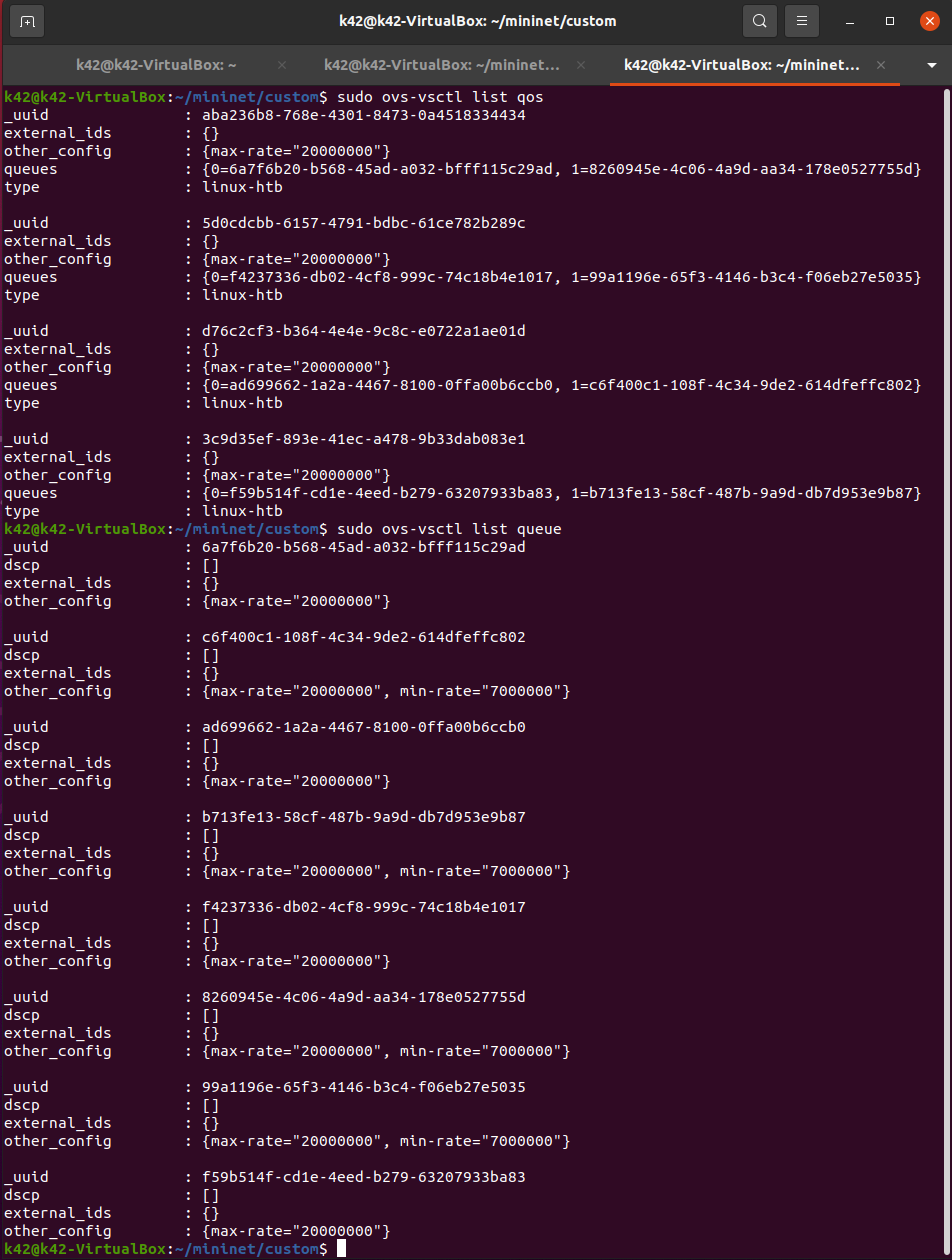
\includegraphics[width=0.7\textwidth]{Bilder/queue-qos}
 \captionsetup{justification=centering}
 \caption{Ausgabe der QoS und Queue der Switches aller Lokationen}
 \label{queue-qos}
\end{figure}

Für den Test wurden zwei weitere VirtualBox-Maschinen mit Ubuntu aufgestellt. Eine Maschine stellt den Server in der Lokation Frankfurt dar. Die andere Maschine stellt einen Host in der Berliner Lokation dar. Beide Maschinen wurden mit der Haupt-VirtualBox-Maschine über eine interne Schnittstelle verbunden. Der Frankfurter Server besitzt die IP \textit{\textbf{192.168.1.18}}, während der Berliner Host die IP \textit{\textbf{192.168.2.15}} besitzt. Dies wurde per Netplan eingerichtet, welcher per \textit{\textbf{sudo apt install netplan.io}} Befehl auf beiden Systemen installiert worden ist. Danach wurden in den Konfigurationsdateien im Dateipfad \textit{\textbf{/etc/netplan/}} die dementsprechende IP-Adresse, das Gateway der Lokation eingegeben und dhcp auf false gestellt. Anschließend wurden die Einstellungen mit dem Befehl \textit{\textbf{sudo netplan apply}} übernommen. Nach den Schritten besteht zwischen dem Host in Berlin und dem Server in Frankfurt über die Haupt-VirtualBox-Maschine eine Verbindung.\par
Um nun die Quality of Service und Queue Konfiguration zu testen, wurde auf dem Server in Frankfurt der Prosody \textit{\textbf{Extensible Messaging and Presence Protocol}} (XMPP) Server installiert und konfiguriert. Dazu wurde der Befehl \textit{\textbf{sudo apt-get install prosody}} im Terminal eingegeben. Anschließend wurde der Server anhand der Datei im Pfad \textit{\textbf{/etc/prosody/prosody.cfg.lua}} konfiguriert und mit dem Befehl \textit{\textbf{sudo systemctl restart prosody-service}} neu gestartet. Nun läuft in der Frankfurter Lokation ein XMPP-Server. Des Weiteren wurde auf dem Server in Frankfurt und auf dem Host in Berlin der XMPP-Client Pidgin mit dem Befehl \textit{\textbf{sudo apt install pidgin}} installiert. Es wurde danach über Prosody zwei XMPP-Benutzer mit dem Befehl \textit{\textbf{sudo prosodyctl adduser user1@192.168.1.18}} und \textit{\textbf{sudo prosodyctl adduser user2@192.168.1.18}} mit der Eingabe eines Passwortes erstellt. Mit dem Pidgin-Client wurden in beiden Lokationen die Nutzer eingeloggt, die sich zusätzlich gegenseitig zu den Kontakten hinzugefügt haben. Nun waren die Nutzer gegenseitig für einander sichtbar. Jetzt kann per Rechtsklick ein Sprachanruf gestartet und getätigt werden (siehe Abbildung \ref{pidgin}). Während dem Anruf kann per \textit{\textbf{sudo ovs-ofctl dump-flows s1}} Befehl erkannt werden, dass die Anzahl der Pakete für die vorher eingefügte UDP-Bedingung stetig steigen (siehe Abbildung \ref{udp}). Per Wireshark können die zwischen den Standorten Übermittelten UDP-Pakete betrachtet werden (siehe Abbildung \ref{udp2}). Damit wurde gezeigt, dass die UPD-Pakete des Sprachanrufes über die gesetzte Bedingung auf die Queue 1 weitergeleitet wird. Somit erhalten alle Pakete eine minimale Geschwindigkeit von sieben Megabit.

\begin{figure}[H]
 \centering
 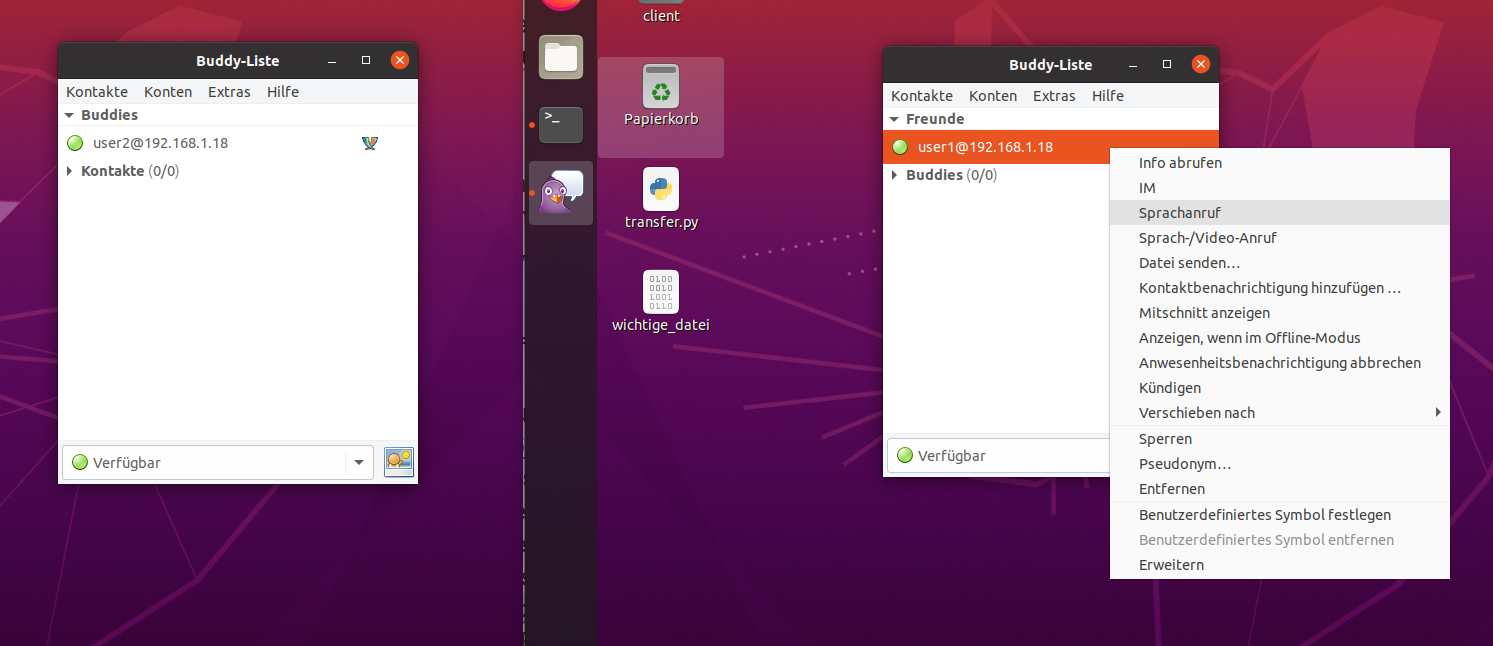
\includegraphics[width=0.8\textwidth]{Bilder/pidgin}
 \captionsetup{justification=centering}
 \caption{Sprachanruf zwischen Berlin und Frankfurt}
 \label{pidgin}
\end{figure}

\begin{figure}[H]
 \centering
 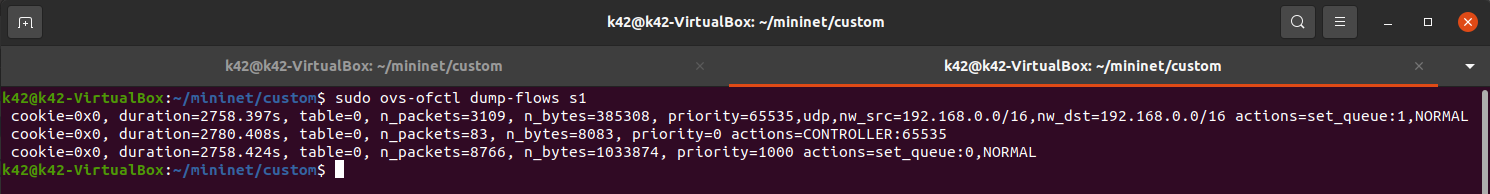
\includegraphics[width=0.8\textwidth]{Bilder/udp}
 \captionsetup{justification=centering}
 \caption{Ausgabe der Flows von s1}
 \label{udp}
\end{figure}

\begin{figure}[H]
 \centering
 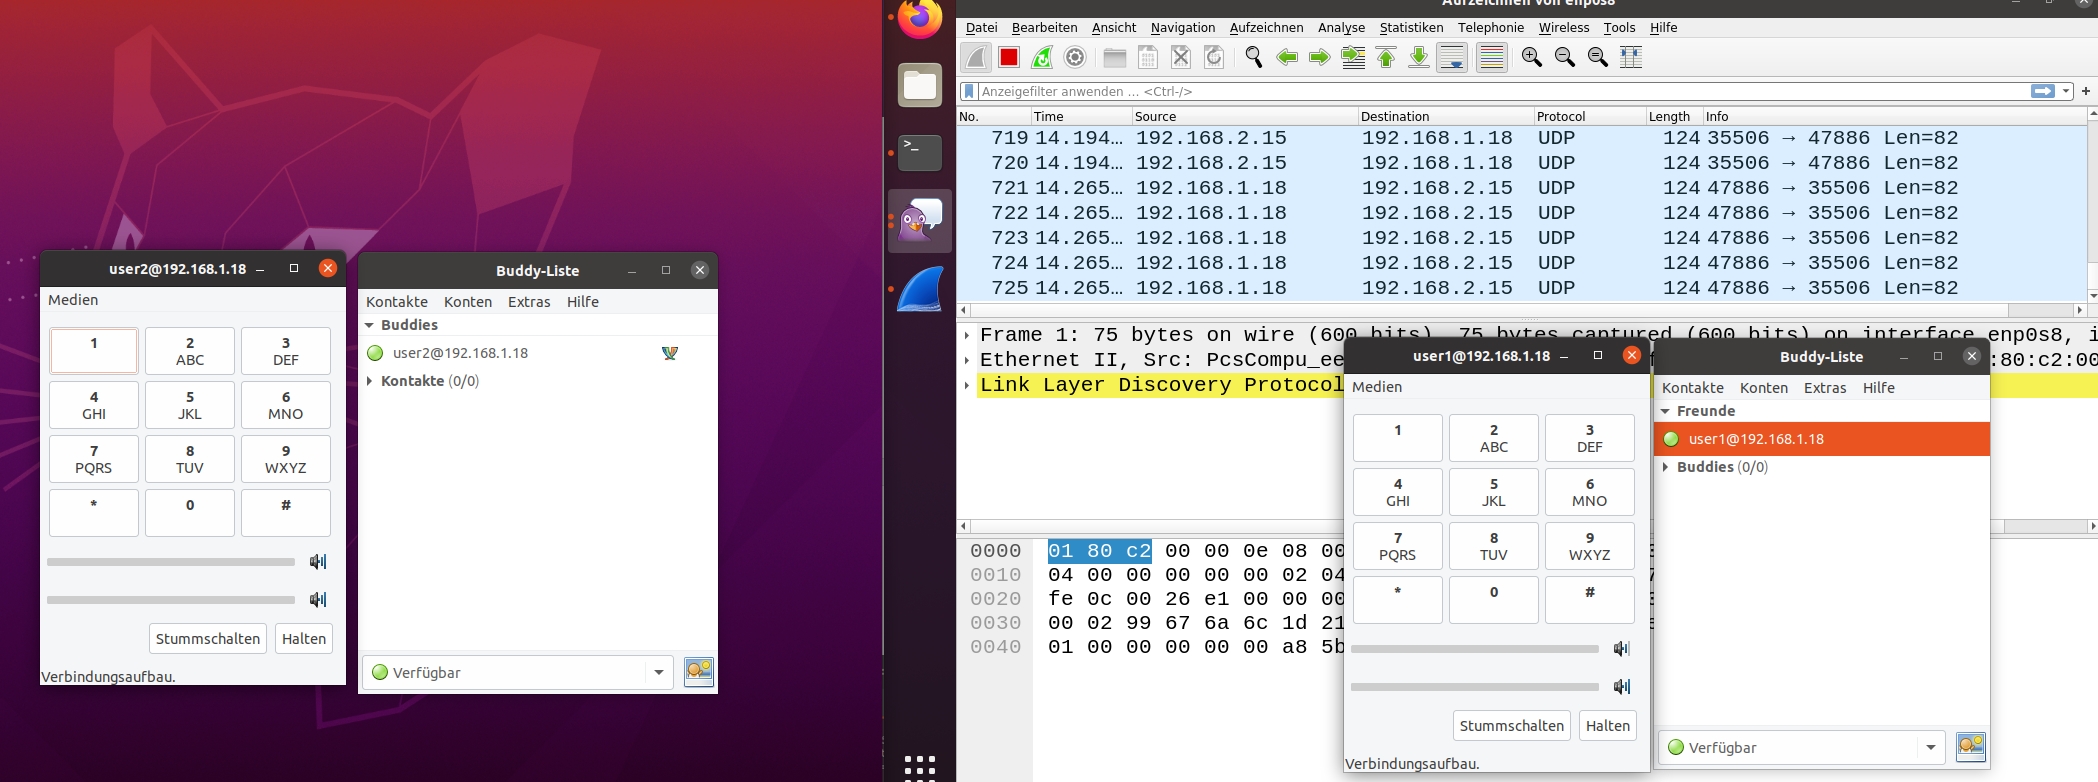
\includegraphics[width=0.8\textwidth]{Bilder/udp2}
 \captionsetup{justification=centering}
 \caption{UDP-Pakete während dem Sprachanruf}
 \label{udp2}
\end{figure}

\newpage
\section{Priorisierung der Datenübertragung über API}
\subsection{Vorüberlegung}
{\tiny Verfasst von: Mücahit\par}
Anhand des Schlüsselwortes \textit{\textbf{priority}} soll der Flow einer Datenübertragung zwischen der Lokation Berlin und Frankfurt priorisiert werden. Allen anderen Flows werden auf der Strecke eine geringere Priorität zugewiesen, sodass die Datenübertragung bevorzugt wird. Falls die gleiche Priorität bei zwei Flows existiert, wird der Flow mit der genaueren Bedingung verwendet \cite{usingovs}. Die Datenübertragung soll über einem in der Zentrale eingerichteten \textit{\textbf{Secure-Shell}} (SSH) Server laufen. Dazu wird auf dem Host in Berlin ein \textit{\textbf{SSH-Client}} benötigt. Bei der Übertragung nutzt SSH üblicherweise den \textit{\textbf{Port 22}} über dem \textit{\textbf{Transport Control Protocol}} (TCP). Mit dieser Information wird die Bedingung für die Priorisierung des Flows festgelegt. Die Übertragung und die Priorisierung werden versucht, in einem ausführbaren Python-Skript zu realisieren, bei der die Angabe der IPv4-Adresse des Hosts in Berlin und des Hosts in der Zentrale als Parameter nötig werden. Es könnte die IPv4-Adresse der Quelle und des Ziels auch automatisch vom Skript durch das System ermittelt werden. Das Skript sollte folgende Schritte beinhalten:
\begin{itemize}
\item[1.] IP-Quelle und Ziel eingeben und einlesen (später -> automatisieren)
\item[2.] Voraussichtlichen Flow über API priorisieren. Restlichen Datenverkehr drosseln
\item[3.] Übertragung per SSH starten
\item[4.] Bei Erfolg Priorisierung und Drosslung wieder aufheben
\item[5.] Bei Fehler Fehlermeldung ausgeben
\end{itemize}
Der Controller, genauer der OpenFlow-Server und der Restserver laufen unter der IP-Adresse \textit{\textbf{192.168.1.20}} und kann von jedem Host erreicht werden. Dies ist wichtig, da die Priorisierung von außen durchgeführt wird. Ansonsten kann der Controller, wenn dieser auf \textit{\textbf{localhost}} läuft, nicht erreicht werden.

\newpage
\subsection{Durchführung}
{\tiny Verfasst von: Mücahit\par}
\begin{wrapfigure}{R}{0.5\textwidth}
	\vspace{-\baselineskip}
 	\centering
 	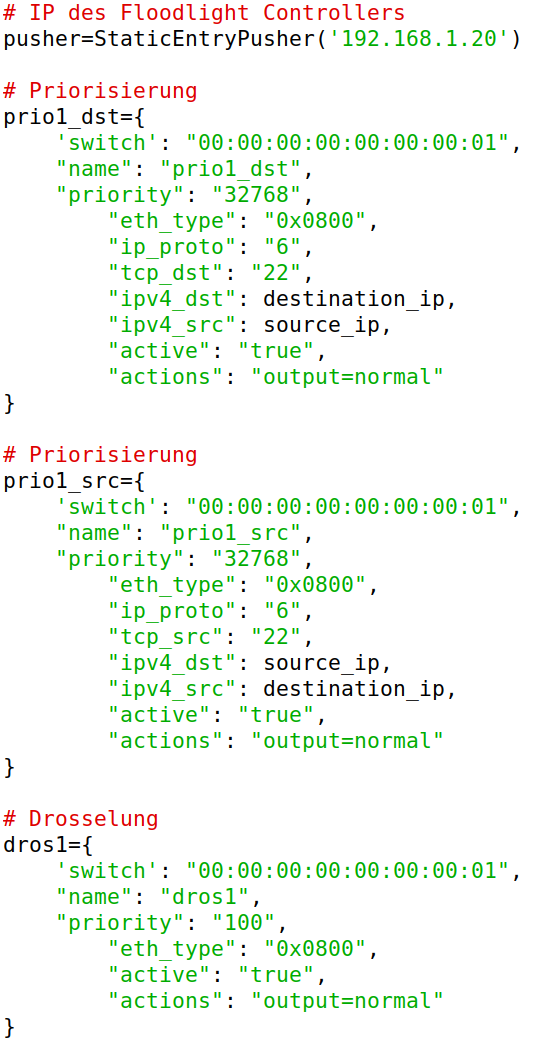
\includegraphics[width=0.4\textwidth]{Bilder/transfer-flow}
 	\caption{Flows für die Priorisierung und die Drosselung}
 	\label{transfer-flow}
\end{wrapfigure}
Die Durchführung erfolgt mit den im vorherigen Kapitel aufgestellten VirtualBox Maschinen. Auf dem Server in Frankfurt wurde per \textit{\textbf{sudo apt install openssh-server}} Befehl der SSH-Server installiert. Dieser wurde eingestellt, auf der IP des Servers zu laufen. Dafür wurde per \textit{\textbf{sudo nano /etc/ssh/sshd\_config}} Befehl in der Konfigurationsdatei des SSH-Servers die IP-Adresse geändert und die Publickeyauthentication ausgeschaltet. Anschließend wurde der SSH-Server-Dienst mit dem Befehl \textit{\textbf{sudo systemctl restart ssh}} neugestartet, um die Einstellungen zu übernehmen. Auf dem Berliner Host wurde per \textit{\textbf{dd if=/dev/zero of=wichtige\_datei bs=50MB count=1}} Befehl eine Dummy-Datei für die Übertragung auf dem Schreibtisch erstellt.\par

Der Server betreibt einen SSH-Server und der Host einen SSH-Client, womit wichtige Dateien übertragen werden. Dafür wurde auf dem Host ein Python-Skript erstellt, welcher näher erläutert wird. Vorher muss per \textit{\textbf{sudo pip install paramiko scp}} Befehl die benötigten Python-Module für die SSH-Verbindung installiert werden. Die Installation geschieht mit pip dem Paketverwaltungsprogramm von Python. Das Skript holt sich automatisch die IP-Adresse des Senders anhand der \textit{\textbf{get\_IP-Methode}} und speichert diese in eine Variable. Anschließend wird die Angabe der Informationen zur Übermittlung verlangt. Dazu gehört der Dateipfad, die IP-Adresse des Empfängers, den Servernamen, das Serverpasswort und den Pfad, wohin die Datei im Ziel gespeichert werden soll (siehe Abbildung \ref{transfer-daten}). Danach wird ein Objekt als Rest-Client zur Übermittlung der Prioritätensetzung erstellt. Dieser bekommt die \textit{\textbf{192.168.1.20}} als IP-Adresse des Controllers gesetzt. Jetzt werden die Flows zur Priorisierung erstellt. Dabei werden jeweils drei gleiche Flows auf den Switch in der Berliner Lokation mit der ID 2 und auf den Switch in der Frankfurter Lokation mit der ID 1 zugewiesen. Die zwei Flows priorisieren TCP-Pakete mit dem Port 22 und der angegebenen Quell- und Zieladresse. Beide Flows decken eingehende und ausgehende Pakete ab und bekommen \textit{\textbf{32768}} als die maximale Priorität gesetzt. Der dritte Flow drosselt den restlichen Verkehr. Hierbei wird nur der Ethernettyp auf IPv4, die Priorität auf \textit{\textbf{100}} und die Queue auf 2 gesetzt (siehe Abbildung \ref{transfer-flow}). Die Queue 2 wurde vorher mit Maximal 2 Megabit eingestellt. Auch ist die Priorität im Vergleich zu der Datenübertragung deutlich gering und wird an nächster Stelle bearbeitet. Die Flows werden nun mit der \textit{\textbf{Set-Methode}} dem Controller über die REST-API übertragen, der diese dann an die Switches zuweist. Nachdem die Priorisierung abgeschlossen ist, wird im nächsten Schritt die Datei per SSH übertragen. Dazu wird im Skript die vom Benutzer vorher gefragten Informationen zur Datenübertragung benutzt, um eine SSH-Verbindung aufzubauen, um die Datei zu senden (siehe Abbildung \ref{ssh}). Nachdem die Übertragung beendet wurde, wird mit der \textit{\textbf{Remove-Methode}} alle Priorisierungen von den Switches über die REST-API entfernt.

\begin{figure}[H]
 \centering
 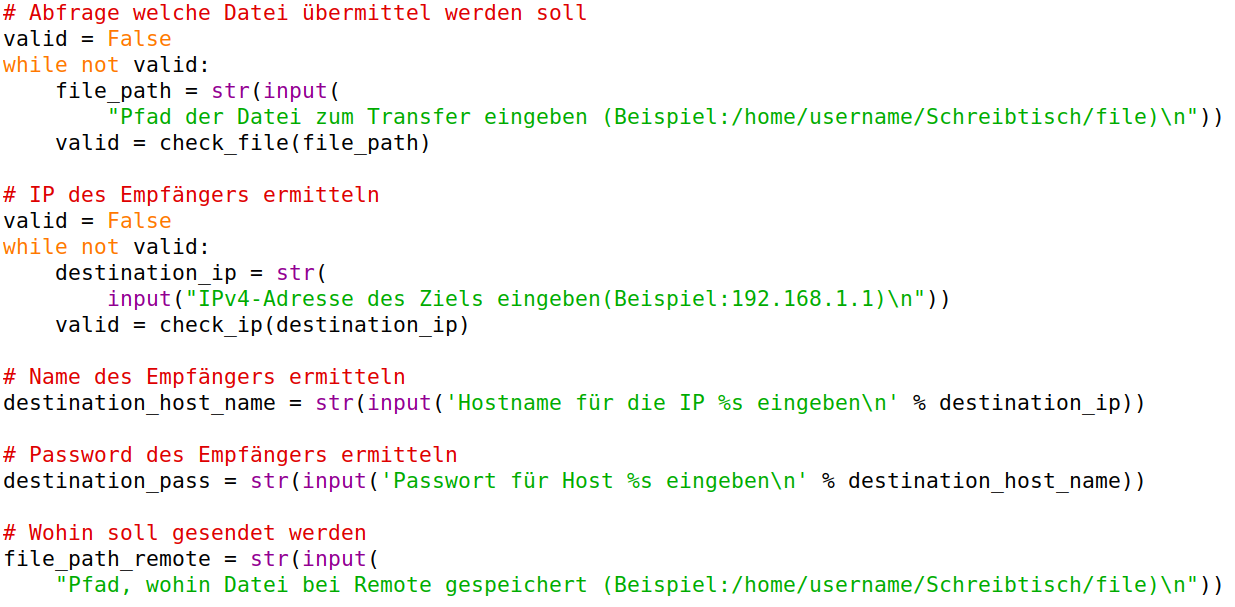
\includegraphics[width=0.8\textwidth]{Bilder/transfer-daten}
 \captionsetup{justification=centering}
 \caption{Abfrage der Daten für den Dateitransfer}
 \label{transfer-daten}
\end{figure}

\begin{figure}[H]
 \centering
 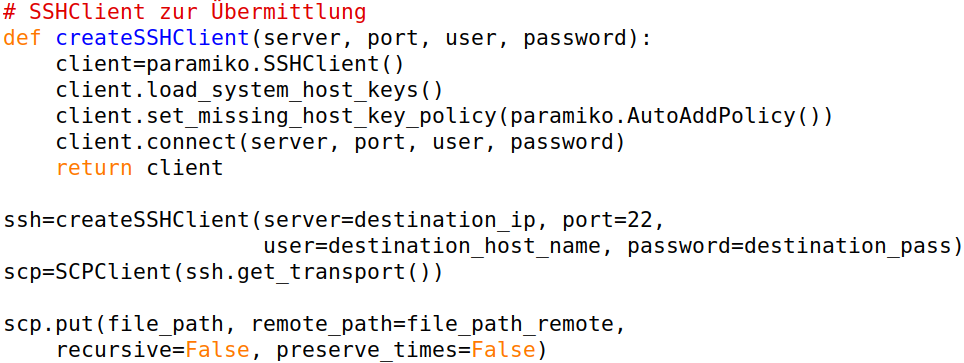
\includegraphics[width=0.8\textwidth]{Bilder/ssh}
 \captionsetup{justification=centering}
 \caption{Übermittlung der Datei über SSH}
 \label{ssh}
\end{figure}

\subsection{Ergebnis}
{\tiny Verfasst von: Mücahit\par}
Über das Python-Skript ist es nun möglich eine Datei priorisiert auf einen Server an der Zentrale zu senden. Das Skript enthält einige Überprüfungen, um beispielsweise zu schauen, ob die eingegebene IP-Adresse und der Dateipfad gültig sind.

\newpage
\section{Analyse weiterer Netzwerkfunktionen}

\subsection{Hub}
{\tiny Verfasst von: Naghmeh\par}
Repeater arbeiten auf der Ebene 1 des OSI-Modells. Seine Aufgabe ist es, das Signal über dasselbe Netz zu regenerieren, bevor es zu schwach oder beschädigt wird, um die Länge von Signalübertragung im selben Netzwerk zu verlängern. Ein Hub ist im Grunde ein Multiport-Repeater. Ein Hub verbindet mehrere Geräte in einem Netzwerk. Hubs können keine Daten filtern, daher werden Pakete an alle verbundenen Geräte gesendet. Darüber hinaus verfügen sie nicht über die Intelligenz, um den besten Pfad für Pakete zu finden, was zu Ineffizienz und Verschwendung führt \cite{networkdevices}.\par
Beim Layer-1-Switching geht es im Wesentlichen um unintelligente Geräte wie Hubs und Repeater. SDN-Switches können so angepasst werden, dass sie sich wie Hubs oder Repeater verhalten. Da Hubs und Repeater keine Informationen speichern können, können Controller bei der Layer-1-Switching keine Datenflüsse weiterleiten. In diesem Fall, jedes Mal, wenn ein Paket ankommt, wird es an den Controller weitergeleitet, der dann entscheidet, alle mit ihm verbundenen Hosts zu überfluten. Dies braucht Zeit, um herauszufinden, wohin das Paket gehen soll, was die Gesamtleistung des Netzes beeinträchtigt \cite{7840116}. Aus diesem Grund wurde keinen Hub oder Repeater in das untersuchende Netzwerk verwendet. 

\subsection{Bridge}
{\tiny Verfasst von: Naghmeh\par}
Eine Bridge in einem Computernetzwerk ist eine Art von Netzwerkgerät, das dazu dient, ein Netzwerk in Abschnitte zu unterteilen. Die Bridges sind dann erforderlich, wenn jedoch Frames von einem physikalischen Netzwerk zu einem anderen weitergeleitet werden sollen. Eine Bridge hat nur zwei Anschlüsse und  arbeitet auf Schicht 2 im OSI-Modell, der Datenverbindungsschicht \cite{baun2019grundlagen}.\par
Das Funktionsprinzip einer Bridge besteht darin, dass sie die Daten abhängig von der MAC-Zieladresse blockiert oder weiterleitet, und diese Adresse wird in jeden Datenrahmen. Eine Bridge verwendet eine Datenbank, um zu bestimmen, wohin der Datenrahmen übertragen werden sollen \cite{networkdevices}.

\subsection{Layer-2-Switch}
{\tiny Verfasst von: Naghmeh\par}
Layer-2-Switch sind ähnlich wie Bridge. Sie verbinden Netze auf Schicht 2 und arbeiten als Brücken, indem sie Tabellen für die Übertragung von Rahmen zwischen Netzen erstellen. Der Zweck der Layer-2-Switch ist es, Daten auf der Grundlage von Flusstabelleneinträgen weiterzuleiten \cite{networkdevices}.\par
Im Falle der Layer-2-Switching, Der Controller ist dafür verantwortlich, den physikalischen Elementen mitzuteilen, wie sie eingehende Datenpakete behandeln sollen. Er ist auch dafür verantwortlich, Datenströme in die Datenstromtabelle des Switches zu schieben. Der Switch ist in der Lage zu lernen, wie Pakete zu behandeln sind, die am Eingangsanschluss ankommen und den Ausgangsanschluss verlassen. Immer wenn ein Paket zum ersten Mal am Eingangsport des Switches ankommt, wird es an den Controller weitergeleitet. Nach dem Empfang eines Pakets, bestimmt der Controller, was damit zu tun ist und ob es weitergeleitet werden soll \cite{7840116}.\par
In dieser Simulation wurden, wie bereits erwähnt, die Open vSwitches verwendet. Open vSwitch ist ein virtueller Mehrschicht-Switch. Er verwendet virtuelle Netzwerkbrücken und Flussregeln, um Pakete zwischen Hosts weiterzuleiten. Er verhält sich wie ein physischer Switch. Ähnlich wie ein herkömmlicher Switch verwaltet OVS Informationen über angeschlossene Geräte wie z. B. die MAC-Adresse \cite{openvswitch1}. Obwohl er nicht nur die Aufgaben von Layer-2-Switch, sondern auch die Aufgaben von Layer-3-Switch durchführen kann, waren für diese Simulation die Funktionalitäten  des Layer-2 Switches ausreichend. Deswegen wurden die 4 Switches als Layer-2-Switch betrachtet.


\subsection{Layer-3-Switch}
{\tiny Verfasst von: James\par}
Da Switching schneller als Routing ist, werden in LANS fast nur mit Switches gearbeitet und an zentralen Stellen Router genutzt, um das Internet zu erreichen. Im Netzwerkplan wurde an jeder Lokation nur ein Switch benötigt, dieser musste nicht VLAN fähig sein. Ein Layer-3-Switch ist beispielsweise ein VLAN-fähiger Switch, der grundlegende Routingfunktionalität bietet und auf Ebene 3 des OSI-Modells arbeitet, die Vermittlungsschicht. Das heißt, ein Layer-3-Switch arbeitet mit IP-Adressen und hat mit der Vermittlung von Paketen zu tun. Innerhalb unseres Projekts entschied man sich keine Layer-3-Switches zu nutzen, da die Funktionalitäten des Layer-2-Switches ausgereicht haben \cite{baun2019grundlagen}.


\subsection{Dynamic Host Configuration Protocol}
\subsubsection{Vorüberlegung}
{\tiny Verfasst von: James\par}
DHCP ist ein Dienst, der an das Netzwerk angeschlossene Geräte mit einer Netzwerkkonfiguration versorgt. Falls ein Gerät eine Konfiguration benötigt, wird dies mithilfe vom DHCP Server konfiguriert, dieser kann beispielsweise im Router des Netzwerks sein. Mithilfe von Mininet konnte eine DHCP Konfiguration realisiert werden. Bis zu diesem Punkt wurde die IP-Adressverwaltung ohne DHCP realisiert. Das heißt, jeder Host musste manuell eine IP-Adresse zugewiesen bekommen. Diese manuelle Konfiguration wurde durch eine for-Schleife im Skript (siehe Abbildung \ref{fororig}) durchgeführt \cite{baun2019grundlagen}.

\begin{figure}[H]
 \centering
 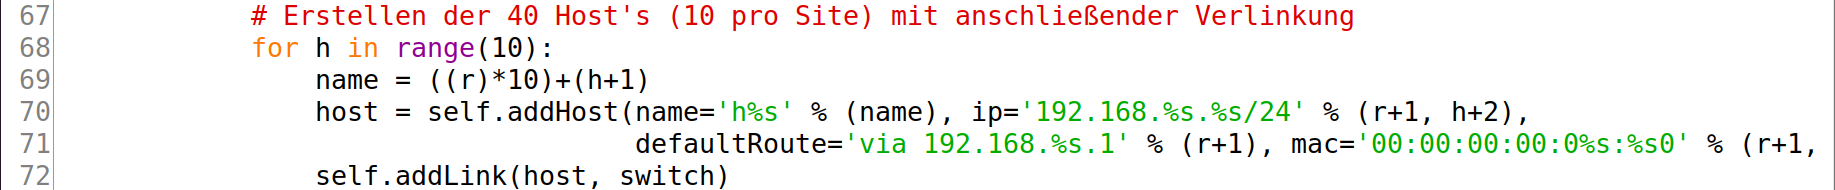
\includegraphics[width=0.8\textwidth]{Bilder/fororig}
 \captionsetup{justification=centering}
 \caption{Statische IP-Adressenverwaltung}
 \label{fororig}
\end{figure}

Bei aktivierten DHCP in Mininet verwaltet der DHCP-Server IP-Adressen ohne manuellen Eingriff des Administrators und weist jedem Host eine IP-Adresse zu. Somit wurde die Funktion der for-Schleife umgeändert, sodass jeder Host von Beginn an die IP-Adresse \textit{\textbf{0.0.0.0}} zugewiesen bekommt. Dadurch wird dem Host keine IP-Adresse manuell zugeteilt. Die IP-Adressverwaltung wird vom DHCP-Server übernommen (siehe Abbildung \ref{forneu}).
  
\begin{figure}[H]
 \centering
 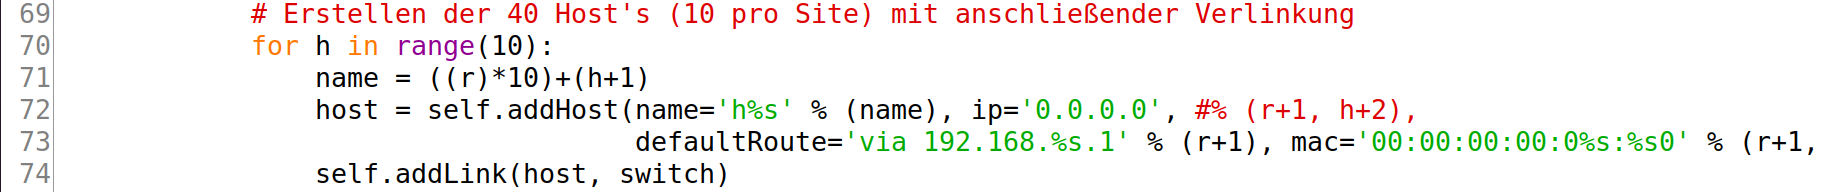
\includegraphics[width=0.8\textwidth]{Bilder/forneu}
 \captionsetup{justification=centering}
 \caption{Dynamische IP-Adressenverwaltung}
 \label{forneu}
\end{figure}

\subsubsection{Durchführung}
{\tiny Verfasst von: James\par}
\begin{wrapfigure}{r}{0.5\textwidth}
	\vspace{-\baselineskip}
 	\centering
 	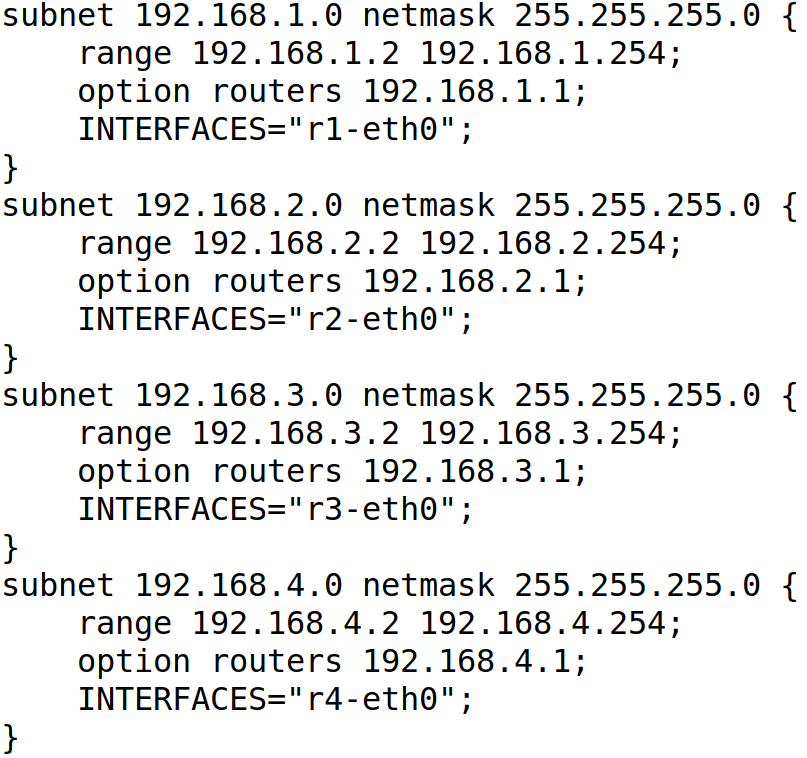
\includegraphics[width=0.4\textwidth]{Bilder/dhcp2}
 	\caption{DHCP-Konfiguration für alle Standorte}
 	\label{dhcp2}
\end{wrapfigure}
Um ein DHCP Server im Netzwerk zu realisieren, muss als erstes der DHCP Server auf die VM installiert werden. Dies wird mit dem Befehl \textit{\textbf{sudo apt-get install isc.dhcp-server}} durchgeführt. Als zweites muss im Mininet-Skript die Zeile \textit{\textbf{os.system(“service isc-dhcp-server restart”)}} ergänzt werden, um den DHCP-Server neu zu starten. Anschließend wird der DHCP server konfiguriert. Dies erfolgt in der \textit{\textbf{dhcpd.conf}} Datei, die sich im Pfad \textit{\textbf{/etc/dhcp}} befindet (siehe Abbildung \ref{dhcp2}). In dieser Datei werden die von den DHCP-Clients benötigten Netzwerkkonfigurationsinformationen gespeichert. Da das Netzwerk aus vier Subnetzen besteht, die mit dem DHCP-Server verbunden sein sollen, müssen vier Subnetze in der \textit{\textbf{dhcpd.conf}} Datei definiert werden. Diese Subnetze benötigen folgende Parameter: \textit{\textbf{subnet, netmask, range, option routers, default-lease-time, max-lease-time}} und \textit{\textbf{INTERFACES}}. Wie in der Tabelle des Netzwerkplans vorgezeigt (siehe Tabelle \ref{netzwerkplan-addressen}), hat jede Lokation eine festgelegte Subnetz IP (\textit{\textbf{subnet}}), Netzwerkmaske (\textit{\textbf{netmask}}) und Router IP (\textit{\textbf{option routers}}) und wird hier definiert. Um allen Hosts in den jeweiligen Subnetzen dynamisch Adressen zuzuweisen, muss innerhalb der Subnetz-Deklaration ein Bereich definiert werden (\textit{\textbf{range}}). Anschließend wird definiert, an welches Netzwerkgerät der DHCP-Server verbunden werden soll (\textit{\textbf{INTERFACES}}). Es kann auch die Gültigkeitsdauer definiert werden, die angibt wie lange einem Host die IP-Adresse zu Verfügung steht. Normalerweise reichen die Voreinstellungen aus, können aber mit \textit{\textbf{default-lease-time}} und \textit{\textbf{max-lease-time}} erhöhen oder herabsetzen, je nach Notwendigkeit. Anhand dieser Informationen, kann für jeden Standort ein Subnetz definiert werden \cite{dhcpd}. 

\subsubsection{Ergebnis}
{\tiny Verfasst von: James\par}
Nachdem das Mininet Skript ausgeführt wird, kann mit Wireshark geprüft werden, ob ein DHCP-Server richtig implementiert wurde. Aus der folgenden Abbildung \ref{wireshark} ist ersichtlich, dass die Pakete zwischen h1 (192.168.1.2) und h11 (192.168.2.2) übertragen werden.
\begin{figure}[H]
 \centering
 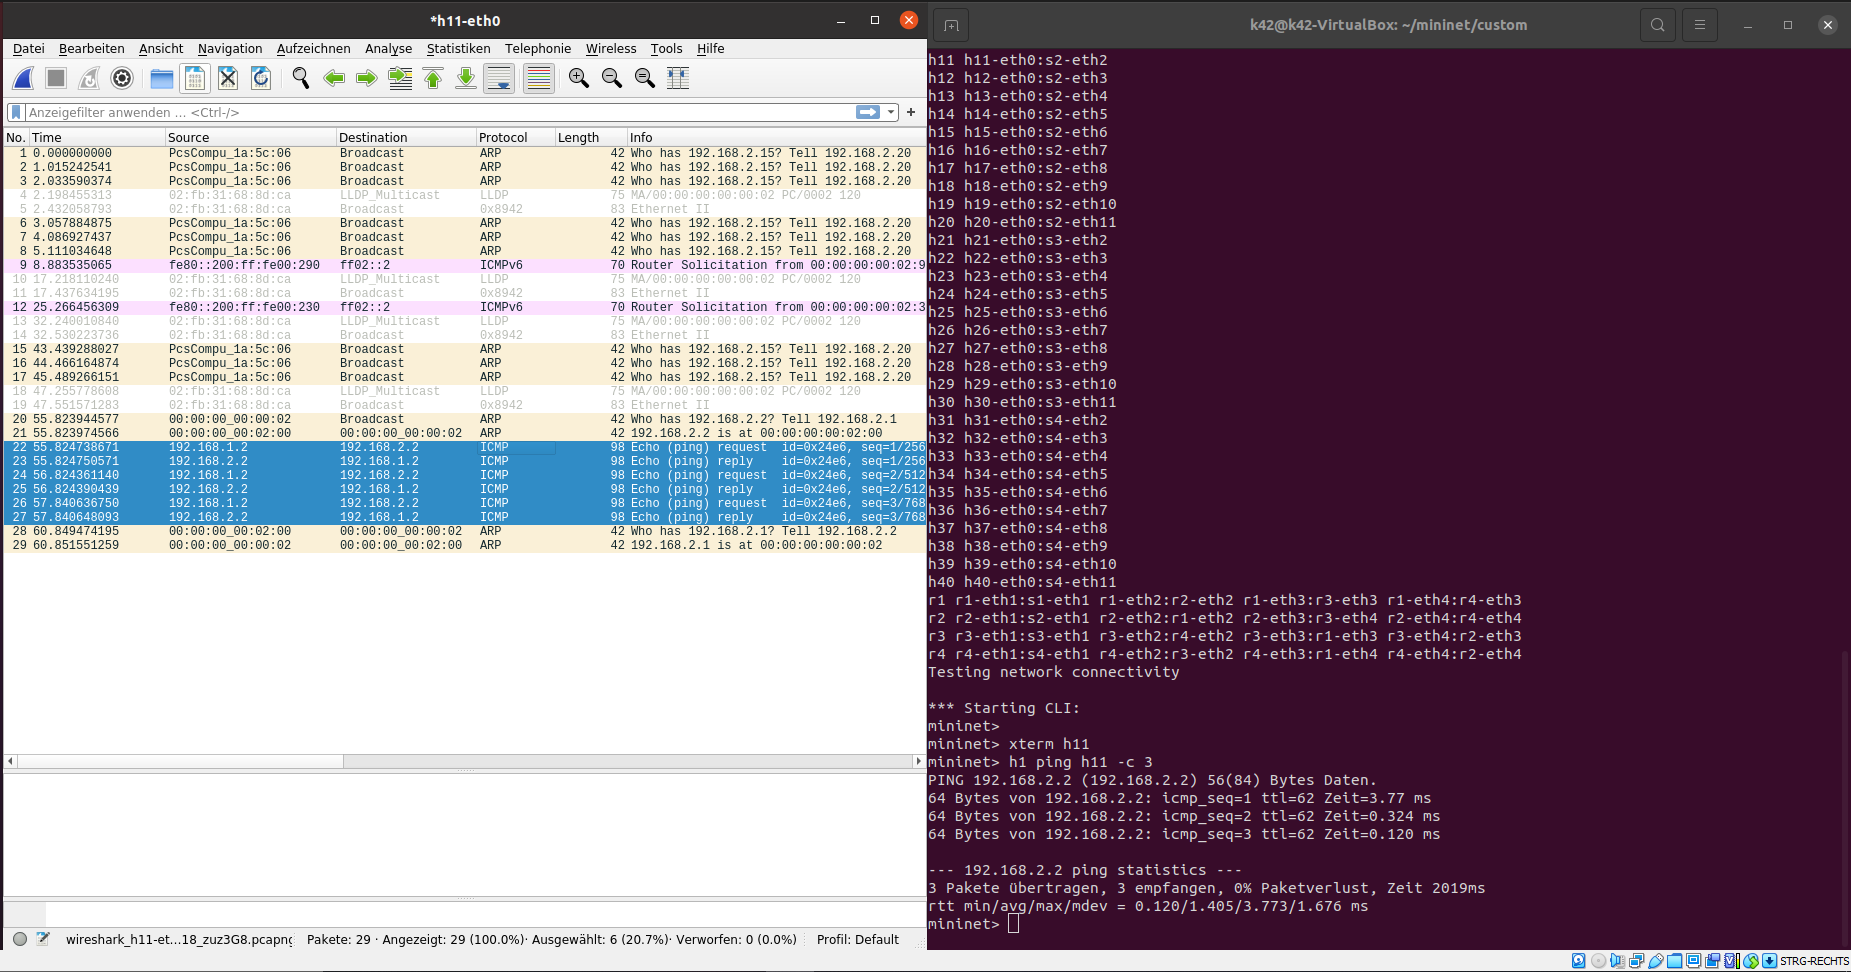
\includegraphics[width=1.0\textwidth]{Bilder/wireshark2}
 \captionsetup{justification=centering}
 \caption{Datenverkehr zwischen h1 und h11}
 \label{wireshark}
\end{figure}

Um die Netzwerkkonfiguration vom DHCP-Server zu betrachten, muss Wireshark vor Mininet gestartet und beim Ausführen des Mininet Skripts eine Switch betrachtet werden. In diesem Beispiel wird die Lokation Frankfurt betrachtet (siehe Abbildung \ref{s1}).

\begin{figure}[H]
 \centering
 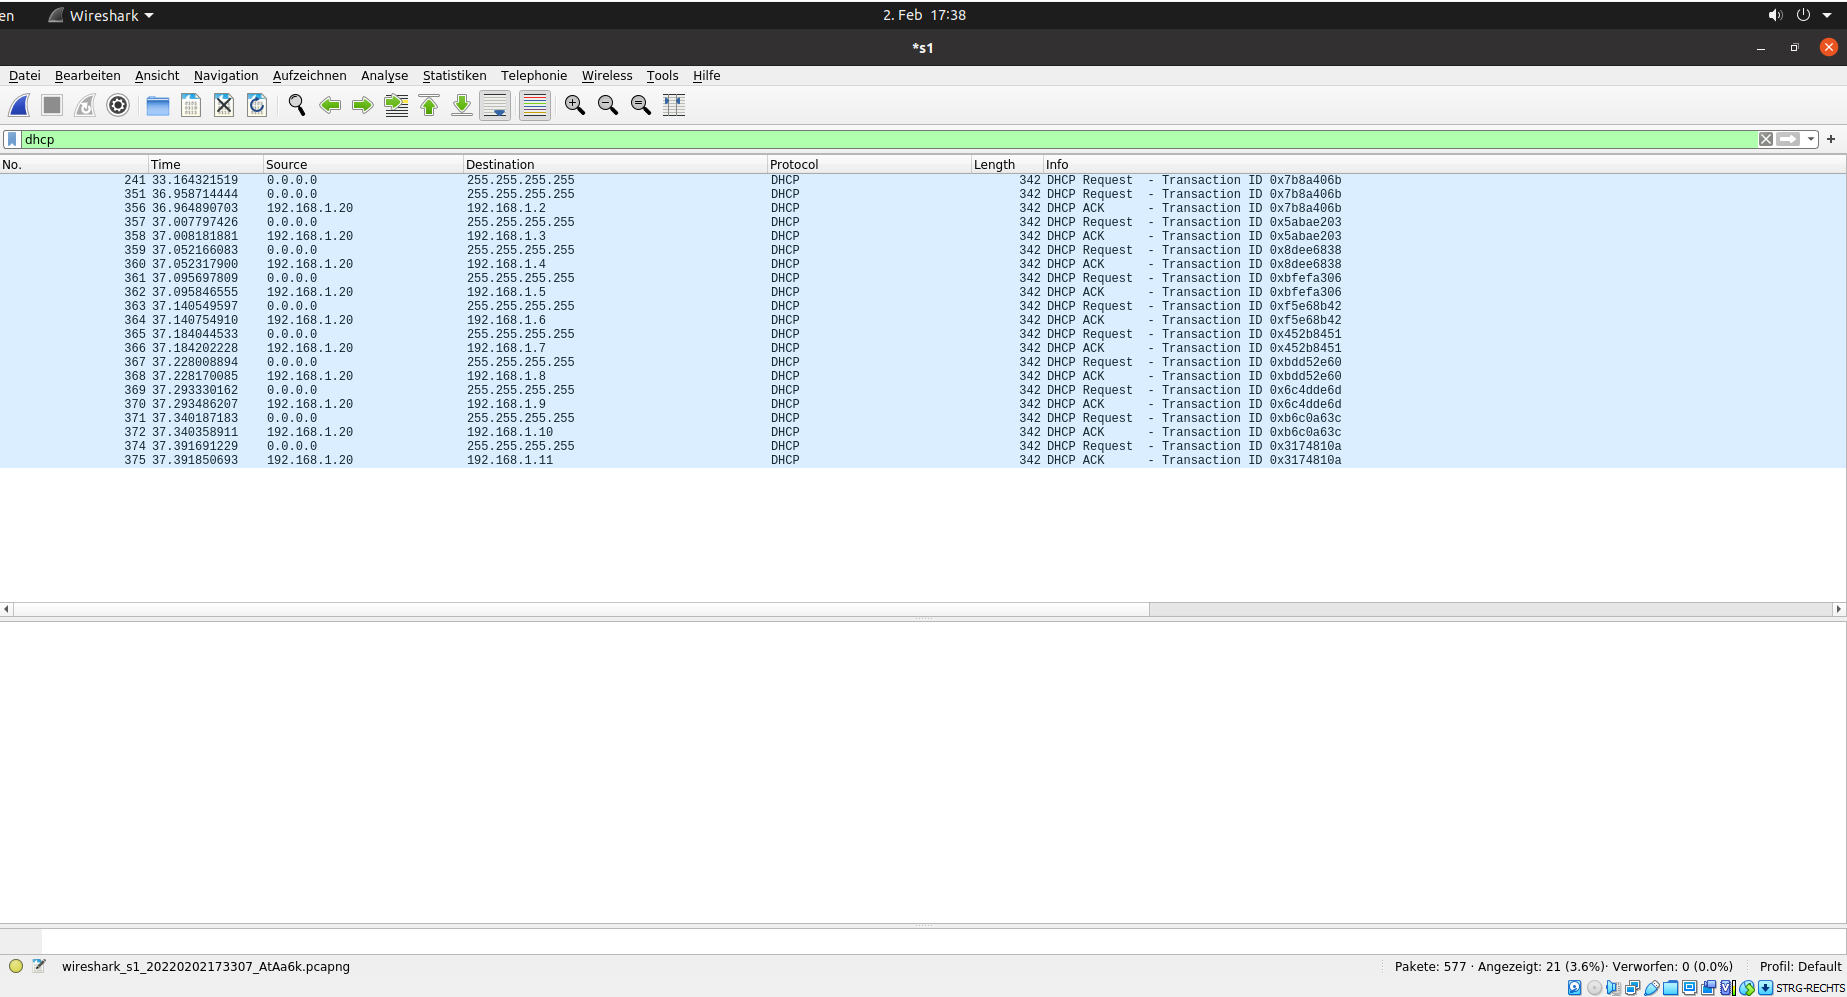
\includegraphics[width=1.0\textwidth]{Bilder/s1}
 \captionsetup{justification=centering}
 \caption{Wireshark-Aufnahme von Switch s1}
 \label{s1}
\end{figure}

\begin{wrapfigure}{r}{0.5\textwidth}
	\vspace{-\baselineskip}
	\centering
	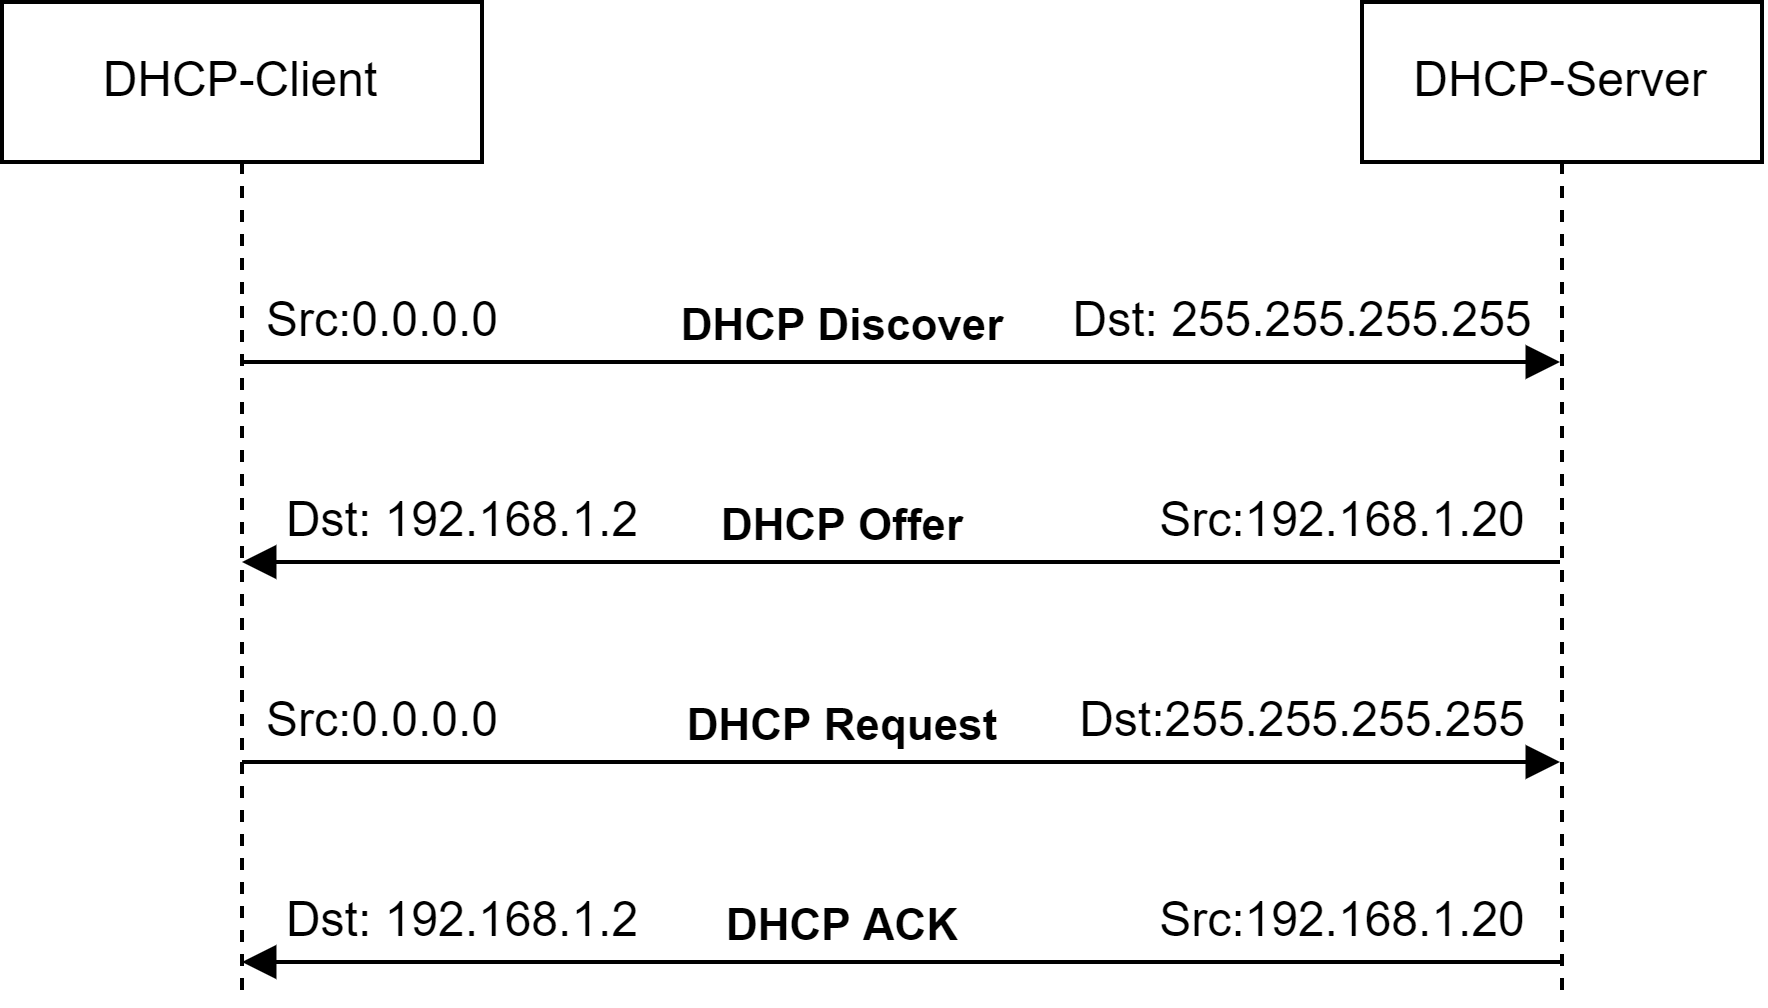
\includegraphics[width=0.6\textwidth]{Bilder/dhcpablauf}
	\caption{Kommunikation zwischen DHCP-Client und DHCP-Server}
	\label{dhcp3}
\end{wrapfigure}

Anhand von Abbildung \ref{s1} sind die gewöhnlichen Schritte vom DHCP Prozess zu erkennen.  
Als erstes schickt ein Client einen \textit{\textbf{Broadcast}} an einem erreichbaren Server (\textit{\textbf{DHCP Discover}}). Die Absender-IP-Adresse ist \textbf{0.0.0.0} und die Zieladresse ist \textbf{255.255.255.255}. Der voreingestellte DHCP-Server empfängt den \textit{\textbf{Broadcast}} und antwortet (\textit{\textbf{DHCP Offer}}). Diese Antwort wird an die angebotene IP-Adresse ({\textbf{192.168.1.2}) gesendet (\textit{\textbf{Unicast}}). Der Client nimmt per Broadcast (\textbf{255.255.255.255}) das Angebot an (\textit{\textbf{DHCP Request}}). Der Server akzeptiert die Adressanfrage an (\textit{\textbf{ACK}}) und speichert im Adresspool die IP als vergeben ab \cite{baun2019grundlagen}. 
\newpage %kannst weg machen falls nicht notwendig

Die übermittelten Informationen vom DHCP Prozess werden im Pfad \textit{\textbf{/var/lib/dhcp/}} gespeichert.  Die Datei \textit{\textbf{dhcpd.leases}} ist eine DHCP client Datenbank, die eine Reihe von lease Deklarationen enthält. Wenn ein lease erworben, erneuert oder freigegeben wird, kann man dies in der Datei einsehen \cite{dhcpd2}. In der Datei \textit{\textbf{dhclient.leases}} werden alle gültigen leases gespeichert\cite{dhclient}.Somit kann der Schritt \textit{\textbf{DHCP Discover}} bei einem wiederholten Durchlauf innerhalb der Lease-Time übersprungen werden, da der Client seine IP-Adresse schon erhalten hat \cite{leases} (siehe Abbildung \ref{wireshark2}). 

\begin{figure}[H]
	\centering
	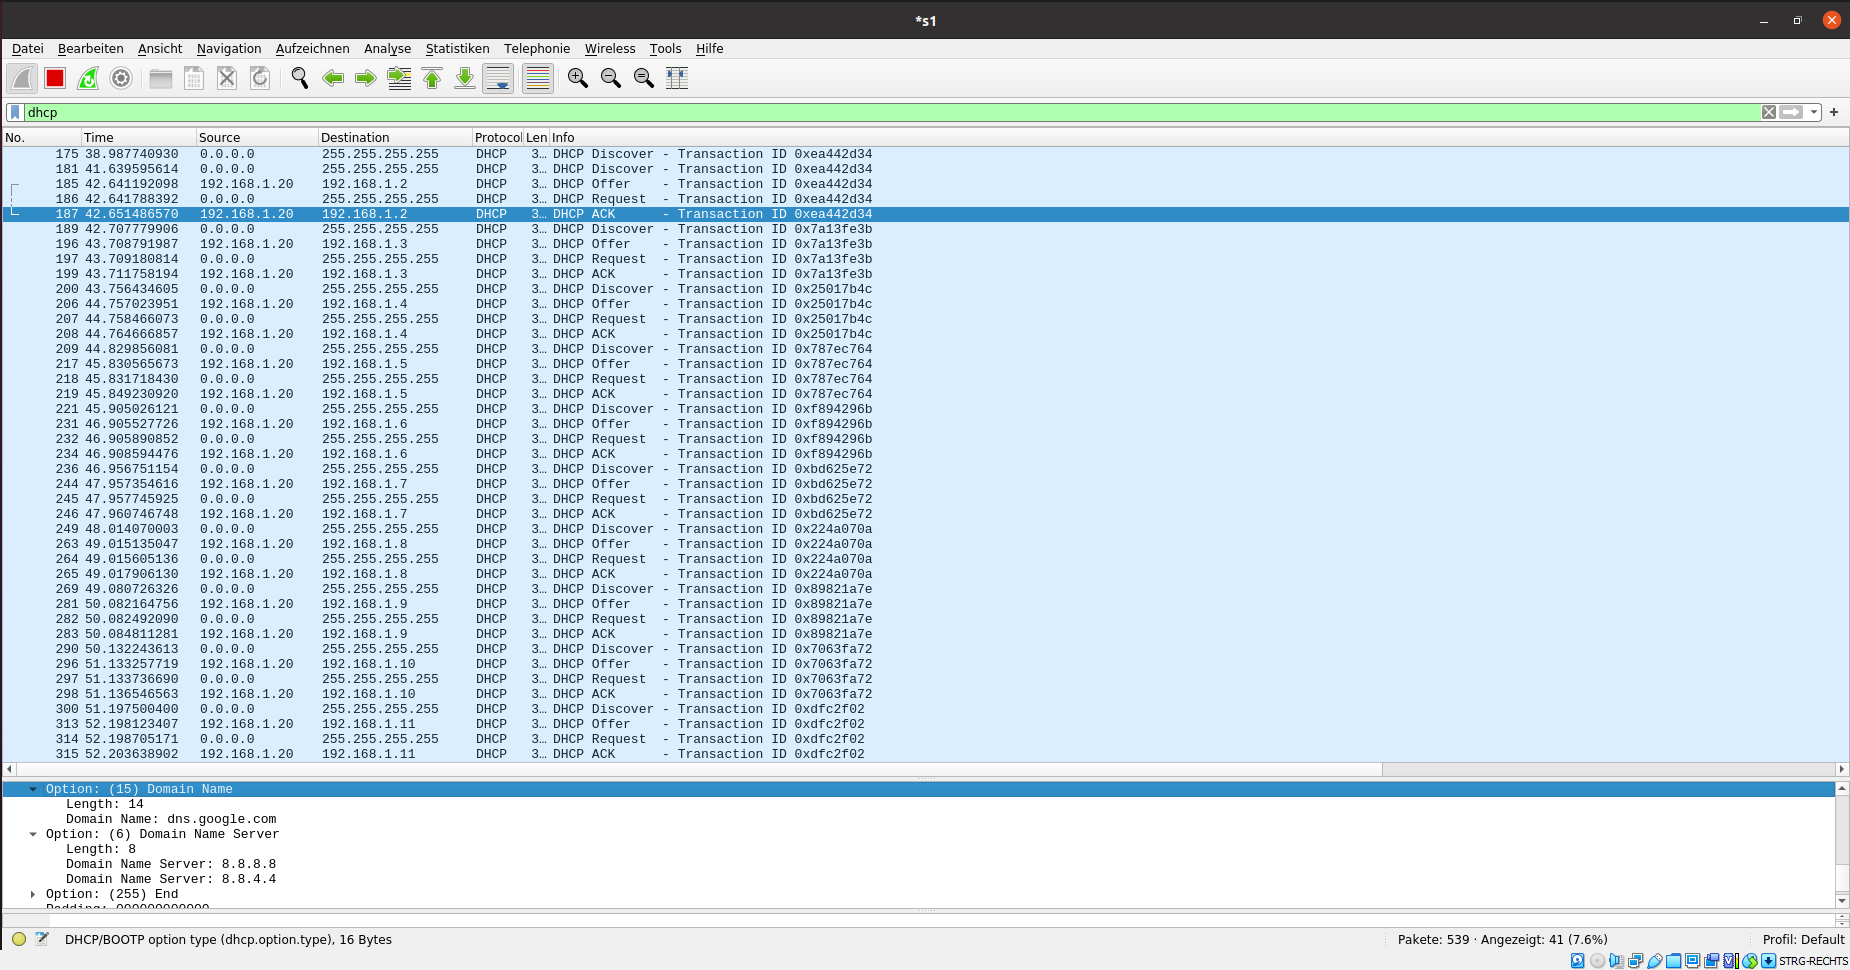
\includegraphics[width=1.0\textwidth]{Bilder/wireshark}
	\captionsetup{justification=centering}
	\caption{Wireshark-Aufnahme vom gekürzten DHCP Prozess}
	\label{wireshark2}
\end{figure}
Falls die Protokolle \textit{\textbf{DHCP Discover}} und \textit{\textbf{DHCP Offer}} nicht übersprungen werden sollen, können die zuständigen Dateien \textit{\textbf{dhcpd.leases}} und \textit{\textbf{dhclient.leases}} gelöscht werden. Diese werden beim nächsten Durchlauf neu erstellt.
\begin{figure}[H]
	\centering
	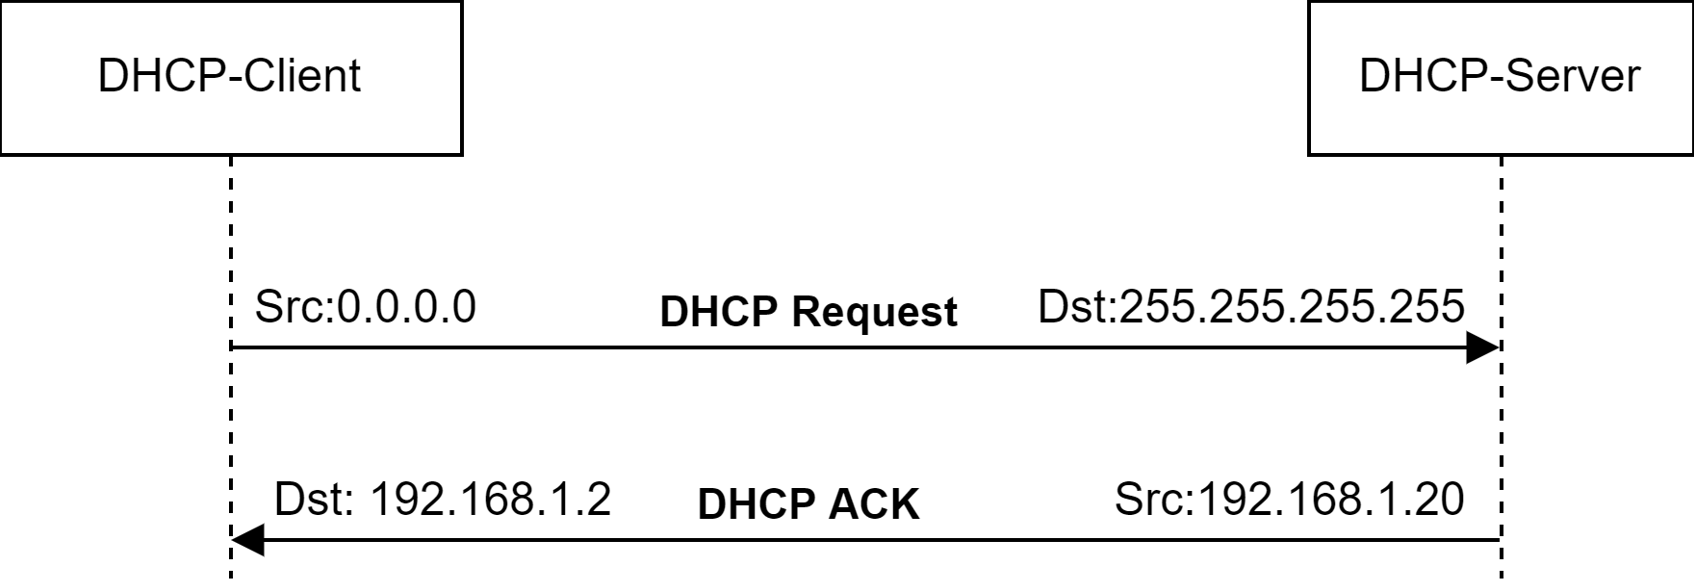
\includegraphics[width=0.5\textwidth]{Bilder/dhcpshort}
	\captionsetup{justification=centering}
	\caption{Kommunikation zwischen DHCP-Client und DHCP-Server}
	\label{s1}
\end{figure}
\newpage

\subsection{Domain Name System}
\subsubsection{Vorüberlegung}
{\tiny Verfasst von: James\par}

Durch das DNS-Protokoll werden Domainnamen zu IP-Adressen umgewandelt \cite{baun2019grundlagen}. Dies wurde bei der Einrichtung des NAT-Firewalls manuell implementiert, sodass Hosts die Möglichkeit haben, nicht nur per IPv4 auf das Internet zugreifen zu können. Es wurde die IP-Adresse des DNS-Servers in die Datei \textit{\textbf{/etc/resolvconf/resolv.conf/head}} eingetragen und gespeichert. Zudem kann mithilfe des implementierten DHCP Servers und dem dhclient auch ein Ergebnis erzielt werden.  
\subsubsection{Durchführung}
{\tiny Verfasst von: James\par}

\begin{wrapfigure}{R}{0.5\textwidth}
	\vspace{-\baselineskip}
	\centering
	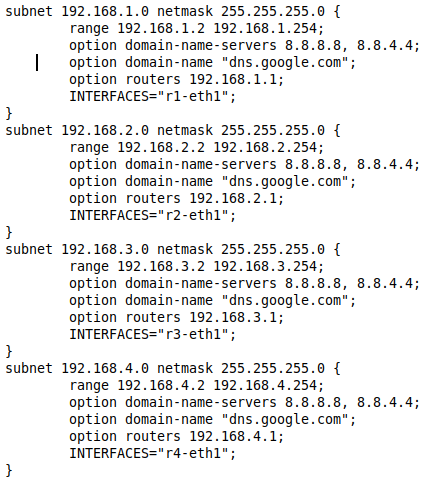
\includegraphics[width=0.4\textwidth]{Bilder/dns}
	\caption{DHCP-Konfiguration für alle Standorte}
	\label{dns}
\end{wrapfigure}
Es werden innerhalb der \textit{\textbf{dhcpd.conf}} Datei im Pfad \textit{\textbf{/etc/dhcp/}} zwei Zeilen in jedem Subnetz hinzugefügt. Mit \textit{\textbf{option domain-name-servers 8.8.8.8, 8.8.4.4;}} wird der verfügbare DNS Server für den Client definiert. Durch \textit{\textbf{option domain-name “dns.google.com”;}} wird der Domänenamen angegeben, der zur Auflösung von Hostnamen verwendet werden soll \cite{dhcpd} (siehe \ref{dns}). Es kann auch der dhclient genutzt werden, um einen DNS Server zu definieren \cite{dhclient2}. Im Pfad /etc/dhcp/ befindet sich die dhclient.conf Datei, die mit prepend domain-name-servers 8.8.8.8 ergänzt werden muss \cite{dhclient3}. \par

\newpage
\subsubsection{Ergebnis}
{\tiny Verfasst von: James\par}
Die Übermittlung des Domain Namen und des Servers kann beobachtet werden, indem die DHCP Protokolle in Wireshark betrachtet werden \cite{dhcpd3}(siehe Abbildung \ref{dns2}).  

\begin{figure}[H]
	\centering
	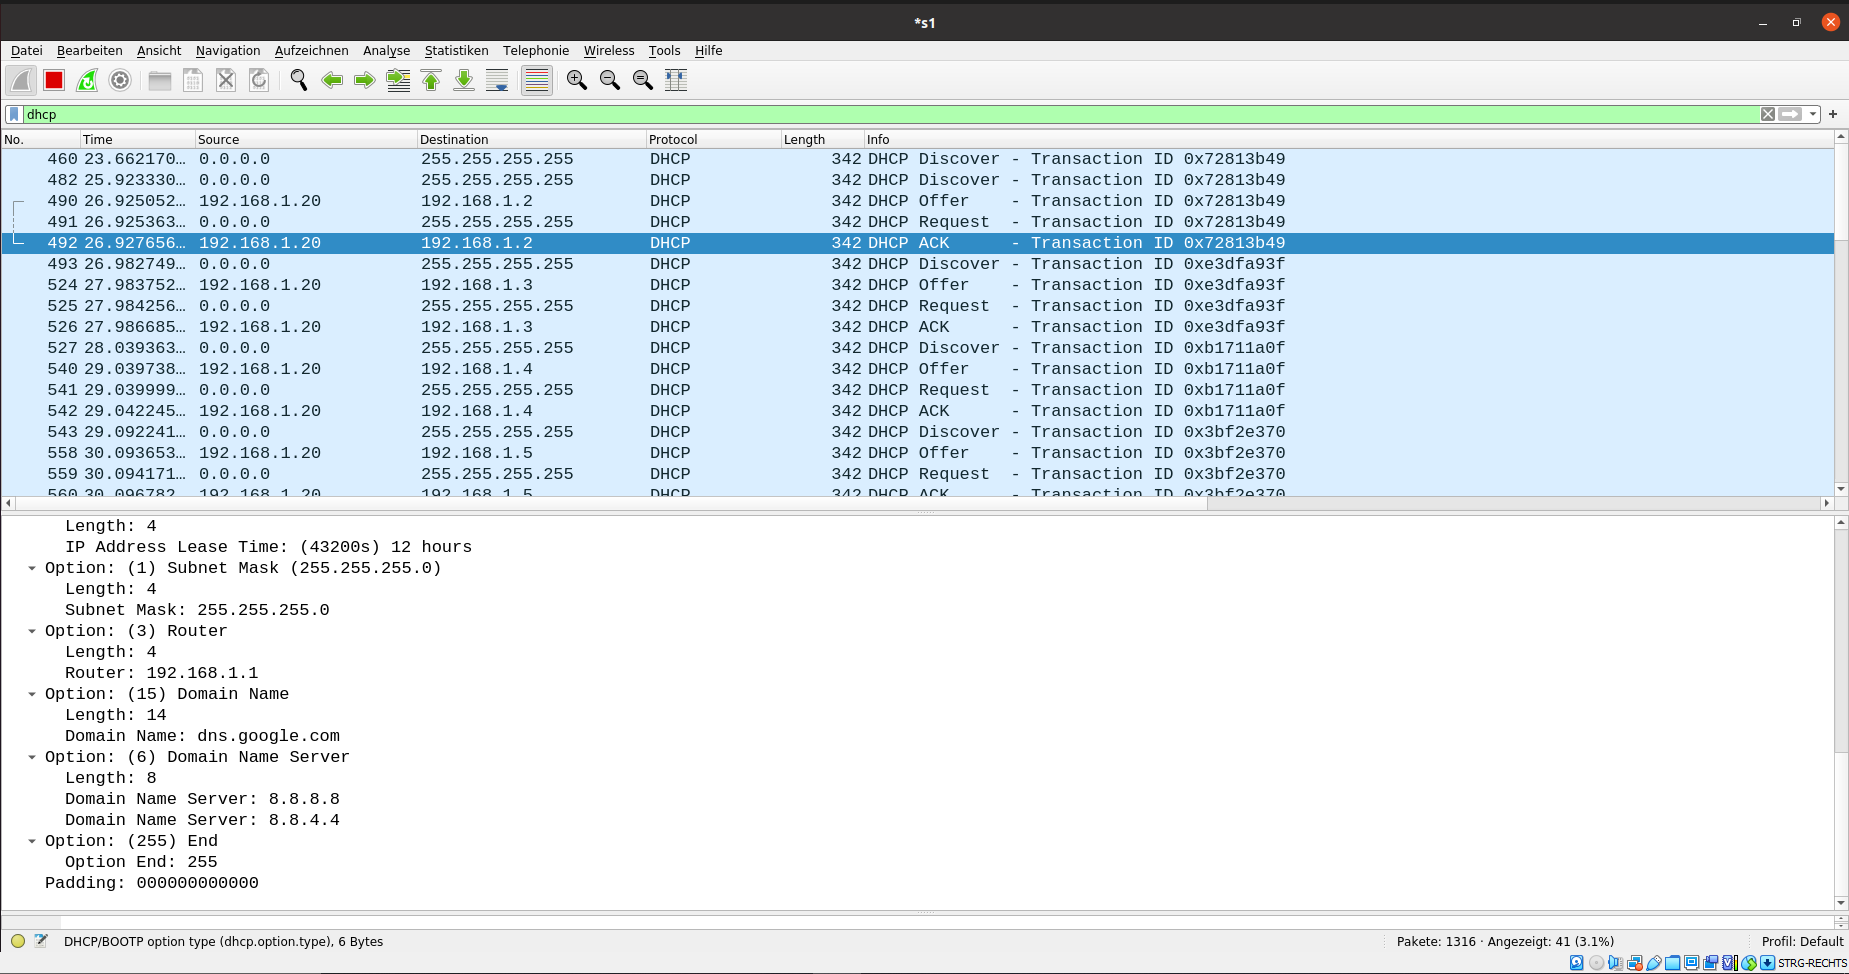
\includegraphics[width=1\textwidth]{Bilder/dns2}
	\captionsetup{justification=centering}
	\caption{Im DHCP ACK Protokoll werden die DNS Informationen vermittelt}
	\label{dns2}
\end{figure}

Nachdem Mininet gestartet wurde, kann mithilfe von \textit{\textbf{systemd-resolve –status}} der genutzte DNS Server betrachtet werden \cite{system}(Siehe Abb. \ref{dns3}).
\begin{figure}[H]
	\centering
	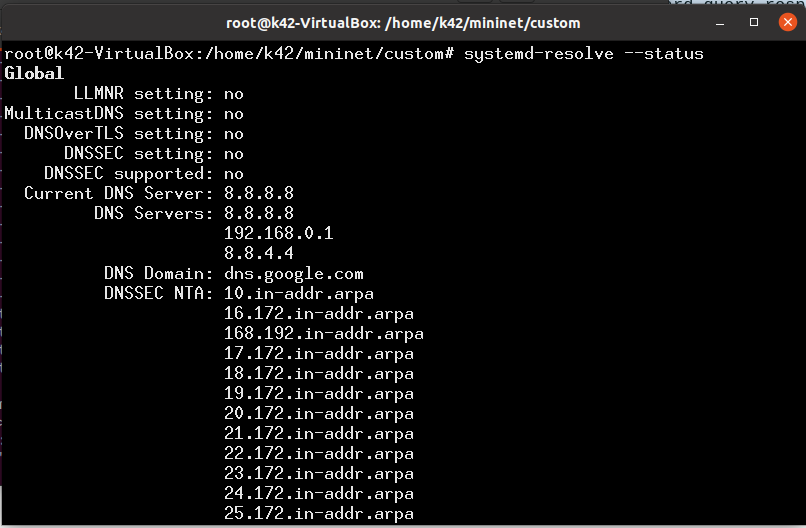
\includegraphics[width=0.64\textwidth]{Bilder/dns3}
	\captionsetup{justification=centering}
	\caption{Terminalausgabe von h1}
	\label{dns3}
\end{figure}

\newpage
\chapter{Diskussion der Ergebnisse}
{\tiny Verfasst von: James\par}
Am Anfang des Projektberichtes wurde von einer “dramatischen Zunahme der Netzwerkkomplexität” gesprochen, wobei eine traditionelle Vorgehensweise der Netzwerkadministration ineffizient sei. Mithilfe des Konzepts SDN, sollte eine effizientere Methode der Netzwerkadministration realisiert werden. Durch die Lösung der Problemstellungen konnten diese zugrunde gelegte Behauptung bestätigt werden. Beispielsweise mussten vier Lokationen realisiert werden, also wurde zu Beginn eine Lokation mit den gewünschten Funktionen erstellt. Anschließend wurden Kopien dieser Lokation für alle weiteren Lokationen genutzt. Durch die Strategie eine kleinstmögliche Umgebung mit den gewünschten Kriterien zu konstruieren, erleichterte es die Vorgehensweise auf Ergebnisse zu kommen. Mininet und der Floodlight Controller ermutigten diese Vorgehensweise, da die Anpassungen leicht umsetzbar waren. Während der Durchführung der Problemstellungen wurde auch festgestellt, dass viele manuelle Einrichtungen mithilfe von SDN automatisiert werden konnten. Die erforschten Ergebnisse werden hier nochmals zusammengefasst und die automatisierten Netzwerkfunktionen durch SDN mit den manuellen Vorgehensweisen verglichen. Anschließend wird kritisch reflektiert, was in der Durchführung mithilfe von SDN nicht reibungslos funktioniert hat.  
\section{Analyse der Ergebnisse}
{\tiny Verfasst von: James\par}
Bei der Verschlüsselung der Netzwerkverbindung zwischen den einzelnen Lokationen konnte über Mininet zwischen den Routern von jedem Standort die VPN Verbindung hergestellt werden. Anstatt eine manuelle Verschlüsselung an jedem Router einzurichten, konnte zentralisiert über Mininet ein Ergebnis erzielt werden. Um private IP-Adressen auf öffentliche IP-Adressen abbilden zu lassen, musste ein NAT eingerichtet werden. Normalerweise wird dies mit der firewalling software \textit{\textbf{iptables}} umgesetzt. Mit \textit{\textbf{iptables}} werden Regeln definiert die für das Filtern und Modifizieren von Paketen zuständig sind. Diese manuelle Einrichtung des NAT-Firewalls an einem Router konnte mithilfe von Mininet übersprungen werden und automatisiert im Skript ergänzt werden. Somit regelt Mininet die Anbindung von einem privaten Netz über \textit{\textbf{NAT}} an das Internet bei jedem Standort. Der Aufbau eines zentralen Topologie-Viewers des Netzwerkes konnte mit dem standardinstallierten Floodlight-Modul dargestellt werden. Indem die Benutzeroberfläche des Controllers in einem Webbrowser aufgerufen wird und auf den Reiter \textit{\textbf{Topology}} klickt, wird eine Topologie dargestellt. Die Erstellung der Topologie vom Controller ist nur möglich, da der Controller die verbundenen Links von den Hosts und den Switches erkennt. Die Realisierung einer zentralen Monitoring Lösung konnte durch eine Konfigurationsänderung in Mininet erstellt werden. Dadurch hatte jeder Netzwerkteilnehmer auf Nagios Core und dem Floodlight Controller Zugriff bekommen. Anstatt manuell bei jedem Netzwerkteilnehmer dies einstellen zu müssen, konnte durch eine Ergänzung des Mininet Skripts die Konfiguration automatisch für alle Hosts eingestellt werden. Eine QoS Funktion innerhalb eines Netzwerkes ohne SDN zu realisieren, ist sehr aufwendig und enthält viele Beschränkungen. Mit SDN kann wegen der zentralisierten Struktur eine Queueliste erstellt werden, die bestimmten Datenverkehr selbst bei begrenzter Netzwerkkapazität priorisiert. Diese Idee wurde mit zwei verschiedenen \textit{\textbf{Queues}} nachgeahmt. Audio- und Videokonferenzen wurden in einer \textit{\textbf{Queue}} definiert und der restliche Datenverkehr in einer anderen. Umgesetzt wurde es im Mininet Skript. Zudem konnte durch eine weitere Ergänzung des Skripts eine Priorisierung der Datenübertragung hergestellt werden. Bei einer Datenübertragung zwischen Berlin und Frankfurt sollte der Datenaustausch priorisiert und alle parallel dazu laufenden Datenübertragungen gedrosselt werden. Indem ein SSH Client in Berlin und ein SSH Server in Frankfurt eingerichtet wird, konnte mithilfe eines Python Skripts auf dem Host die gewünschte Prioritätensetzung ins Netzwerk implementiert werden. Die Realisierung eines DHCP Servers sowohl eines DNS-Dienst für jede Lokation kann automatisiert werden. Somit kann durch Änderung des Mininet Skripts und der \textit{\textbf{dhcpd.conf}} sowie \textit{\textbf{dhclient.conf}} Datei ein DHCP Server und DNS-Dienst realisiert werden. Dies erspart die Zeit an jeder Lokation eine manuelle Konfiguration durchzuführen und kann in einer Weise implementiert werden, dass beim Ausführen des Mininet Skripts die Dienste für alle Hosts konfiguriert werden. \par
Bei einer Änderung der vorgelegten Anforderungen, wie beispielsweise eine \textit{\textbf{Quality of Service Funktion}} von einer anderen Datenübertragung, kann dies durch SDN und mithilfe des Mininet Skript leicht verändert werden. Somit müsste ein Administrator nicht alle Schnittstellen umprogrammieren, sondern kann effizienter in einem automatisierten Schritt das Netzwerk ändern.
\section{Kritische Betrachtung}
{\tiny Verfasst von: James\par}
Obwohl SDN viele Vorteile hat, war der Einstieg in das Thema sehr zeitaufwendig. Viele Installationsanleitungen haben auf Anhieb nicht funktioniert und mussten individuell mit Alternativen Möglichkeiten angepasst werden. Vorkonfigurierte VMs mit mininet und einem  Floodlight Controller haben nicht funktioniert, somit musste selbstständig eine VM konstruiert werden. Zudem war die Vorstellung des Netzwerkes zu Beginn anders als das am Ende erstellte Ergebnis, da SDN viele Funktionalitäten und Alternativmöglichkeiten besitzt. Dadurch kann eine Art der Entscheidungslähmung entstehen, da die Optionen und Einstellungen sehr vielfältig sind. Da der Floodlight Controller in SDN an zentraler Stelle steht, müssen alle Konfigurationen korrekt eingestellt werden. Es muss logischerweise der Controller konstant im Hintergrund laufen und wenn der Controller ausfällt, fällt das gesamte System aus. Das heißt, der Controller muss fehlersicher und mit allen Lokationen verbunden sein. Der Floodlight Controller befindet sich im Netzwerkplan am Standort Frankfurt, jedoch sollte in der Theorie ein zweiter Controller an einer anderen Lokation existieren, der beim Ausfall des Frankfurter Controllers einspringt.  

\chapter{Fazit}\label{ch:fazit}
{\tiny Verfasst von: James, Naghmeh \par}
Auf Grundlage einer umfassenden Recherche, die Durchführung von neun definierten Aufgabenstellungen sowie ein daraus resultierendes Ergebnis sind neue Erkenntnisse über das Konzept SDN für die Gruppenmitglieder gewonnen worden. Ziel dieses Projektes war es nicht nur die Aufgaben zu lösen, sondern verstehen zu können, warum das Konzept SDN die Zukunft von Netzwerkadministration sein könnte.   \par

Nach der Installation und Konfiguration der notwendigen Tools wie die VMs, Mininet und dem Floodlight-Controller und einer erfolgreichen Analyse der Aufgaben hat die Ausarbeitung des Projektes angefangen. Bei der Verschlüsselung des Datenverkehrs zwischen Lokationen wurde die Methode \textit{\textbf{IPSEC over GRE}} implementiert und wurde damit ein Site-to-Site-VPN Verbindung hergestellt. Da die Lokationen über einen Tunnel durch das Internet miteinander verbunden sind, benötigen alle Lokationen eine DSL-Verbindung. Neben einer DSL-Leitung war auch eine Standleitung für alle Lokationen erforderlich. Nach einiger Recherche, Nachfragen und Vergleiche wurde eine passende Wahl für die DSL-Leitung und Standleitung gefunden. NAT-Firewall wurden am Router jeder Lokation implementiert. Das Programm \textit{\textbf{iptable}} wurde umgesetzt, um Regeln für die jeweiligen Router zu definieren. Mithilfe von Mininet wurden Einrichtungen des NAT-Firewalls implementiert, anstatt manuell an jedem Router im Skript dies umzusetzen. Somit ist Mininet zuständig für die Anbindung von einem privaten Netz über \textit{\textbf{NAT}} an das Internet. Eine andere Anforderung für die Sicherstellung des Systems war die Implementierung einer Web Proxy Funktion. Die HTTP und HTTPS Anfragen der Hosts wurden durch den Proxy durchgeführt und die Antwort an dem Host weitergeleitet. Jedoch konnte die Web Proxy Funktion zum Schluss nicht korrekt implementiert werden. Für das zentrale Monitoring wurde Nagios Core verwendet. Dies ermöglicht die Überprüfung der Verfügbarkeit, Geschwindigkeit und Dienste der Netzwerkkomponenten. Bei entstandenen Fehlern werden Administratoren für die Fehlerbehebung benachrichtigt. Mithilfe der \textit{\textbf{Quality of Service}} Funktion ist das Netzwerk in der Lage, Anwendungen und Datenverkehr selbst bei begrenzter Netzwerkkapazität zuverlässig mit hoher Priorität auszuführen. Den Unternehmen war es wichtig, dass bei einer Auslastung des Netzwerkes die Audio- und Videokonferenzen stabil und flüssig laufen. Dafür wurden zwei \textit{\textbf{Queues}} benötigt, einmal für die Audio- und Videokonferenzen(\textit{\textbf{Queue 1}}) und eine für den restlichen Datenverkehr(\textit{\textbf{Queue 0}}). Dies wurde im Mininet Skript umgesetzt. Dabei werden alle UDP Pakete auf die \textit{\textbf{Queue 1}} mit einer minimalen Bandbreite von sieben und einer maximalen Bandbreite von 20 Megabit weitergeleitet. Bei den Bedingungen wurde zusätzlich auch die höchste Priorität eingegeben. Bei den wichtigen Datenübertragungen zwischen Berlin und Frankfurt sollen die Flows priorisiert und alle parallel dazu laufenden Datenübertragungen gedrosselt werden Die Datenübertragung soll über einem in der Zentrale eingerichteten SSH Server laufen. Dazu wird auf dem Host in Berlin und in Frankfurt ein SSH-Client benötigt. Bei der Übertragung nutzt SSH üblicherweise den Port 22 über dem TCP. Mit dieser Information wird die Bedingung für die Priorisierung des Flows festgelegt. Die Datenübertragung und die Priorisierung wurden in einem Python-Skript realisiert. Wegen Mangel an Zeit wurden nur die Netzwerkfunktionen, die die Gesamtleistung des Netzwerks verbessern konnten und notwendig waren, realisiert, wie beispielsweise Layer-2-Switch, DHCP und DNS. Die Layer-2-Switches waren notwendig, um eine Verbindung zum Controller herzustellen und die 10 Hosts in jeder Lokation miteinander zu verbinden. Im Vergleich zu Layer-2-Switches sind Hubs ineffizient für das Netzwerk, da bei jedem Datenverkehr der Controller entscheiden muss, alle mit ihm verbundenen Hosts zu überfluten. Dies beeinträchtigt die Gesamtleistung des Netzwerkes. Deshalb wurde auch kein Hub realisiert. Nach Recherche zeigte sich, dass der Floodlight Controller DHCP unterstützt und umsetzbar ist. Damit konnte ein DHCP Server bei allen Lokationen implementiert werden und die individuelle Konfiguration an jedem Standort musste nicht durchgeführt werden. Innerhalb der Konfiguration des DHCP Servers konnte eine Alternativmöglichkeit für einen DNS-Dienst gefunden werden, der mithilfe von DHCP alle Clients mit einem DNS-Dienst ausstattet. Durch zusätzliche Einstellungen konnte dies realisiert werden. \par 

Aus den Ergebnissen geht hervor, dass durch SDN eine dynamischere Administration möglich ist. Beispielsweise zeigt die Realisierung einer \textit{\textbf{QoS}} Funktion, dass Benutzern bei bestimmten Anwendungen mehr Bandbreite zur Verfügung steht, da eine agile Verwaltung des Datenverkehrs durch SDN ermöglicht wird. Zudem verändert sich durch SDN die Art der Netzwerkkonfiguration. Normalerweise müsste ein Netzwerkadministrator für das Hinzufügen eines Gerätes in einem Netzwerk mehrere Schritte absolvieren, wie die manuelle Konfiguration von Switches und Routern etc.. Mit SDN ist diese Konfiguration programmierbar, sodass viele Konfigurationsschritte automatisiert oder übersprungen werden können. Ebenfalls wichtig ist, dass durch die zentrale Verwaltung des Netzes über den Floodlight Controller eine einfache Einstellung eines Topologie-Viewers ermöglicht wird und dadurch keine weiteren Tools benötigt werden. Aus dem Ergebnis der Priorisierung der Datenübertragung von Berlin nach Frankfurt geht hervor, dass eine Priorisierung der Datenübertragung von einer anderen Lokation nach Frankfurt durch einfache Änderungen auch realisierbar sei. Kleinere Änderungen an der programmierten Konfiguration könnten ausreichen, um ein gleiches Ergebnis zu erzielen. Des Weiteren konnte bei der Einrichtung des NAT-Firewalls sowie bei der \textit{\textbf{VPN}} Einrichtung die verringerte Komplexität der Implementierung nachvollziehbar werden. Aus Wissen von vorherigen Modulen war die Einstellung des NAT-Firewalls auf zwei Host-Maschinen zeitaufwendiger und komplexer als die Realisierung im Projekt. Insbesondere ist die Skalierbarkeit des Netzwerkes effizienter umsetzbar, da automatisierte Voreinstellungen angepasst werden können, um die gewünschte Infrastruktur aufzubauen. Zudem verdeutlichen die Ergebnisse bei der Einstellung vom DHCP Prozess sowie des DNS-Dienstes die vereinfachte Erweiterung von Netzwerkfunktionen.  
\printbibliography[title=Literaturverzeichnis]

\appendix
\chapter{Anhang}

\lstinputlisting[language=Python,
	caption={Das in Python geschrieben Mininet-Skript},
	backgroundcolor = \color{lightgray},
	captionpos=b,
	numbers=left,
	keywordstyle=\color{RoyalBlue},
	rulecolor=\color{black},
	upquote=true, 
	showstringspaces=false,
	breaklines=true,
	frame=single,
	aboveskip=2em,
	label={interface-deklaration},
	%autogobble=true,
	]{Code/site.py}
\captionsetup{justification=centering,margin=2cm}

\newpage
\lstinputlisting[language=Python,
caption={Das in Python geschrieben SSH-Transfer-Skript},
backgroundcolor = \color{lightgray},
captionpos=b,
numbers=left,
keywordstyle=\color{RoyalBlue},
rulecolor=\color{black},
upquote=true, 
showstringspaces=false,
breaklines=true,
frame=single,
aboveskip=2em,
label={interface-deklaration},
%autogobble=true,
]{Code/Transfer.py}
\captionsetup{justification=centering,margin=2cm}

\end{document}